\section{Specifica della componente Presenter} {

	La componente Presenter raccoglie tutti metodi per gestire le operazioni dell'applicazione e si suddivide in due categorie: Client\g~ (vedi \ref{presenter.client}) e Server\g~ (vedi \ref{presenter.server}).

	\subsection{Client}{\label{presenter.client}

	La sotto-componente Client\g~ gestisce le richieste avanzate dalla componente View (vedi \ref{view.client}). A questo scopo dialoga con la sotto-componente Server\g~ del Presenter (vedi \ref{presenter.server}) tramite la messaggi XML\g  (vedi  \ref{par:XMLComm}).\\
	\`E formata dalle classi:
	\begin{itemize}
		\item[] \path{mytalk.client.iPresenter.iUser.iLogicUser.ICommunicationLogic} (sez. \ref{par:ICommunicationLogic})
		\item[] \path{mytalk.client.iPresenter.iUser.iLogicUser.ILogUserLogic} (sez. \ref{par:ILogUserLogic})
		\item[] \path{mytalk.client.iPresenter.iUser.iLogicUser.IRegisterLogic} (sez. \ref{par:IRegisterLogic})
		\item[] \path{mytalk.client.iPresenter.iUser.iLogicUser.IDataUserLogic} (sez. \ref{par:IDataUserLogic})
		\item[] \path{mytalk.client.iPresenter.iUser.iLogicUser.IUpdateViewLogic} (sez. \ref{par:IUpdateViewLogic})
		\item[] \path{mytalk.client.presenter.user.logicUser.CommunicationLogic} (sez. \ref{par:CommunicationLogic})
		\item[] \path{mytalk.client.presenter.user.logicUser.LogUserLogic} (sez. \ref{par:LogUserLogic})
		\item[] \path{mytalk.client.presenter.user.logicUser.RegisterLogic} (sez. \ref{par:RegisterLogic})
		\item[] \path{mytalk.client.presenter.user.logicUser.DataUserLogic} (sez. \ref{par:DataUserLogic})
		\item[] \path{mytalk.client.presenter.user.logicUser.UpdateViewLogic} (sez. \ref{par:UpdateViewLogic})
		\item[] \path{mytalk.client.presenter.iUser.iCommunication.IMediaStream} (sez. \ref{par:IMediaStream})
		\item[] \path{mytalk.client.presenter.iUser.iCommunication.IPeerConnection} (sez. \ref{par:IPeerConnection})
		\item[] \path{mytalk.client.presenter.user.communication.MediaStream} (sez. \ref{par:MediaStream})
		\item[] \path{mytalk.client.presenter.user.communication.PeerConnection} (sez. \ref{par:PeerConnection})
		\item[] \path{mytalk.client.presenter.user.communication.WebRTCAdaptee} (sez. \ref{par:WebRTCAdaptee})
		\item[] \path{mytalk.client.iPresenter.iAdministrator.iLogicAdmin.ILogAdminLogic} (sez. \ref{par:ILogAdminLogic})
		\item[] \path{mytalk.client.iPresenter.iAdministrator.iLogicAdmin.IStatisticLogic} (sez. \ref{par:IStatisticLogic})
		\item[] \path{mytalk.client.iPresenter.iAdministrator.iLogicAdmin.IUpdateViewLogic} (sez. \ref{par:IUpdateViewLogic})
		\item[] \path{mytalk.client.presenter.administrator.logicAdmin.LogAdminLogic} (sez. \ref{par:LogAdminLogic})
		\item[] \path{mytalk.client.presenter.administrator.logicAdmin.StatisticLogic} (sez. \ref{par:StatisticLogic})
		\item[] \path{mytalk.client.presenter.administrator.logicAdmin.UpdateViewLogic} (sez. \ref{par:UpdateViewLogic})
		\item[] \path{mytalk.client.presenter.user.logicUser.common.CommonFunctions} (sez. \ref{par:CommonFunctions})
		\item[] \path{mytalk.client.iPresenter.iUser.iServerComUser.IWebSocketUser} (sez. \ref{par:IWebSocketUser})
		\item[] \path{mytalk.client.presenter.user.serverComUser.WebSocketUser} (sez. \ref{par:WebSocketUser})
	\end{itemize}

	\begin{sloppypar} {

	\subsubsection{Package mytalk.client.iPresenter.iUser.iLogicUser}{
	
\begin{figure}[h!tbp]
		\centering
		\label{fig:presenterLogicUser}
		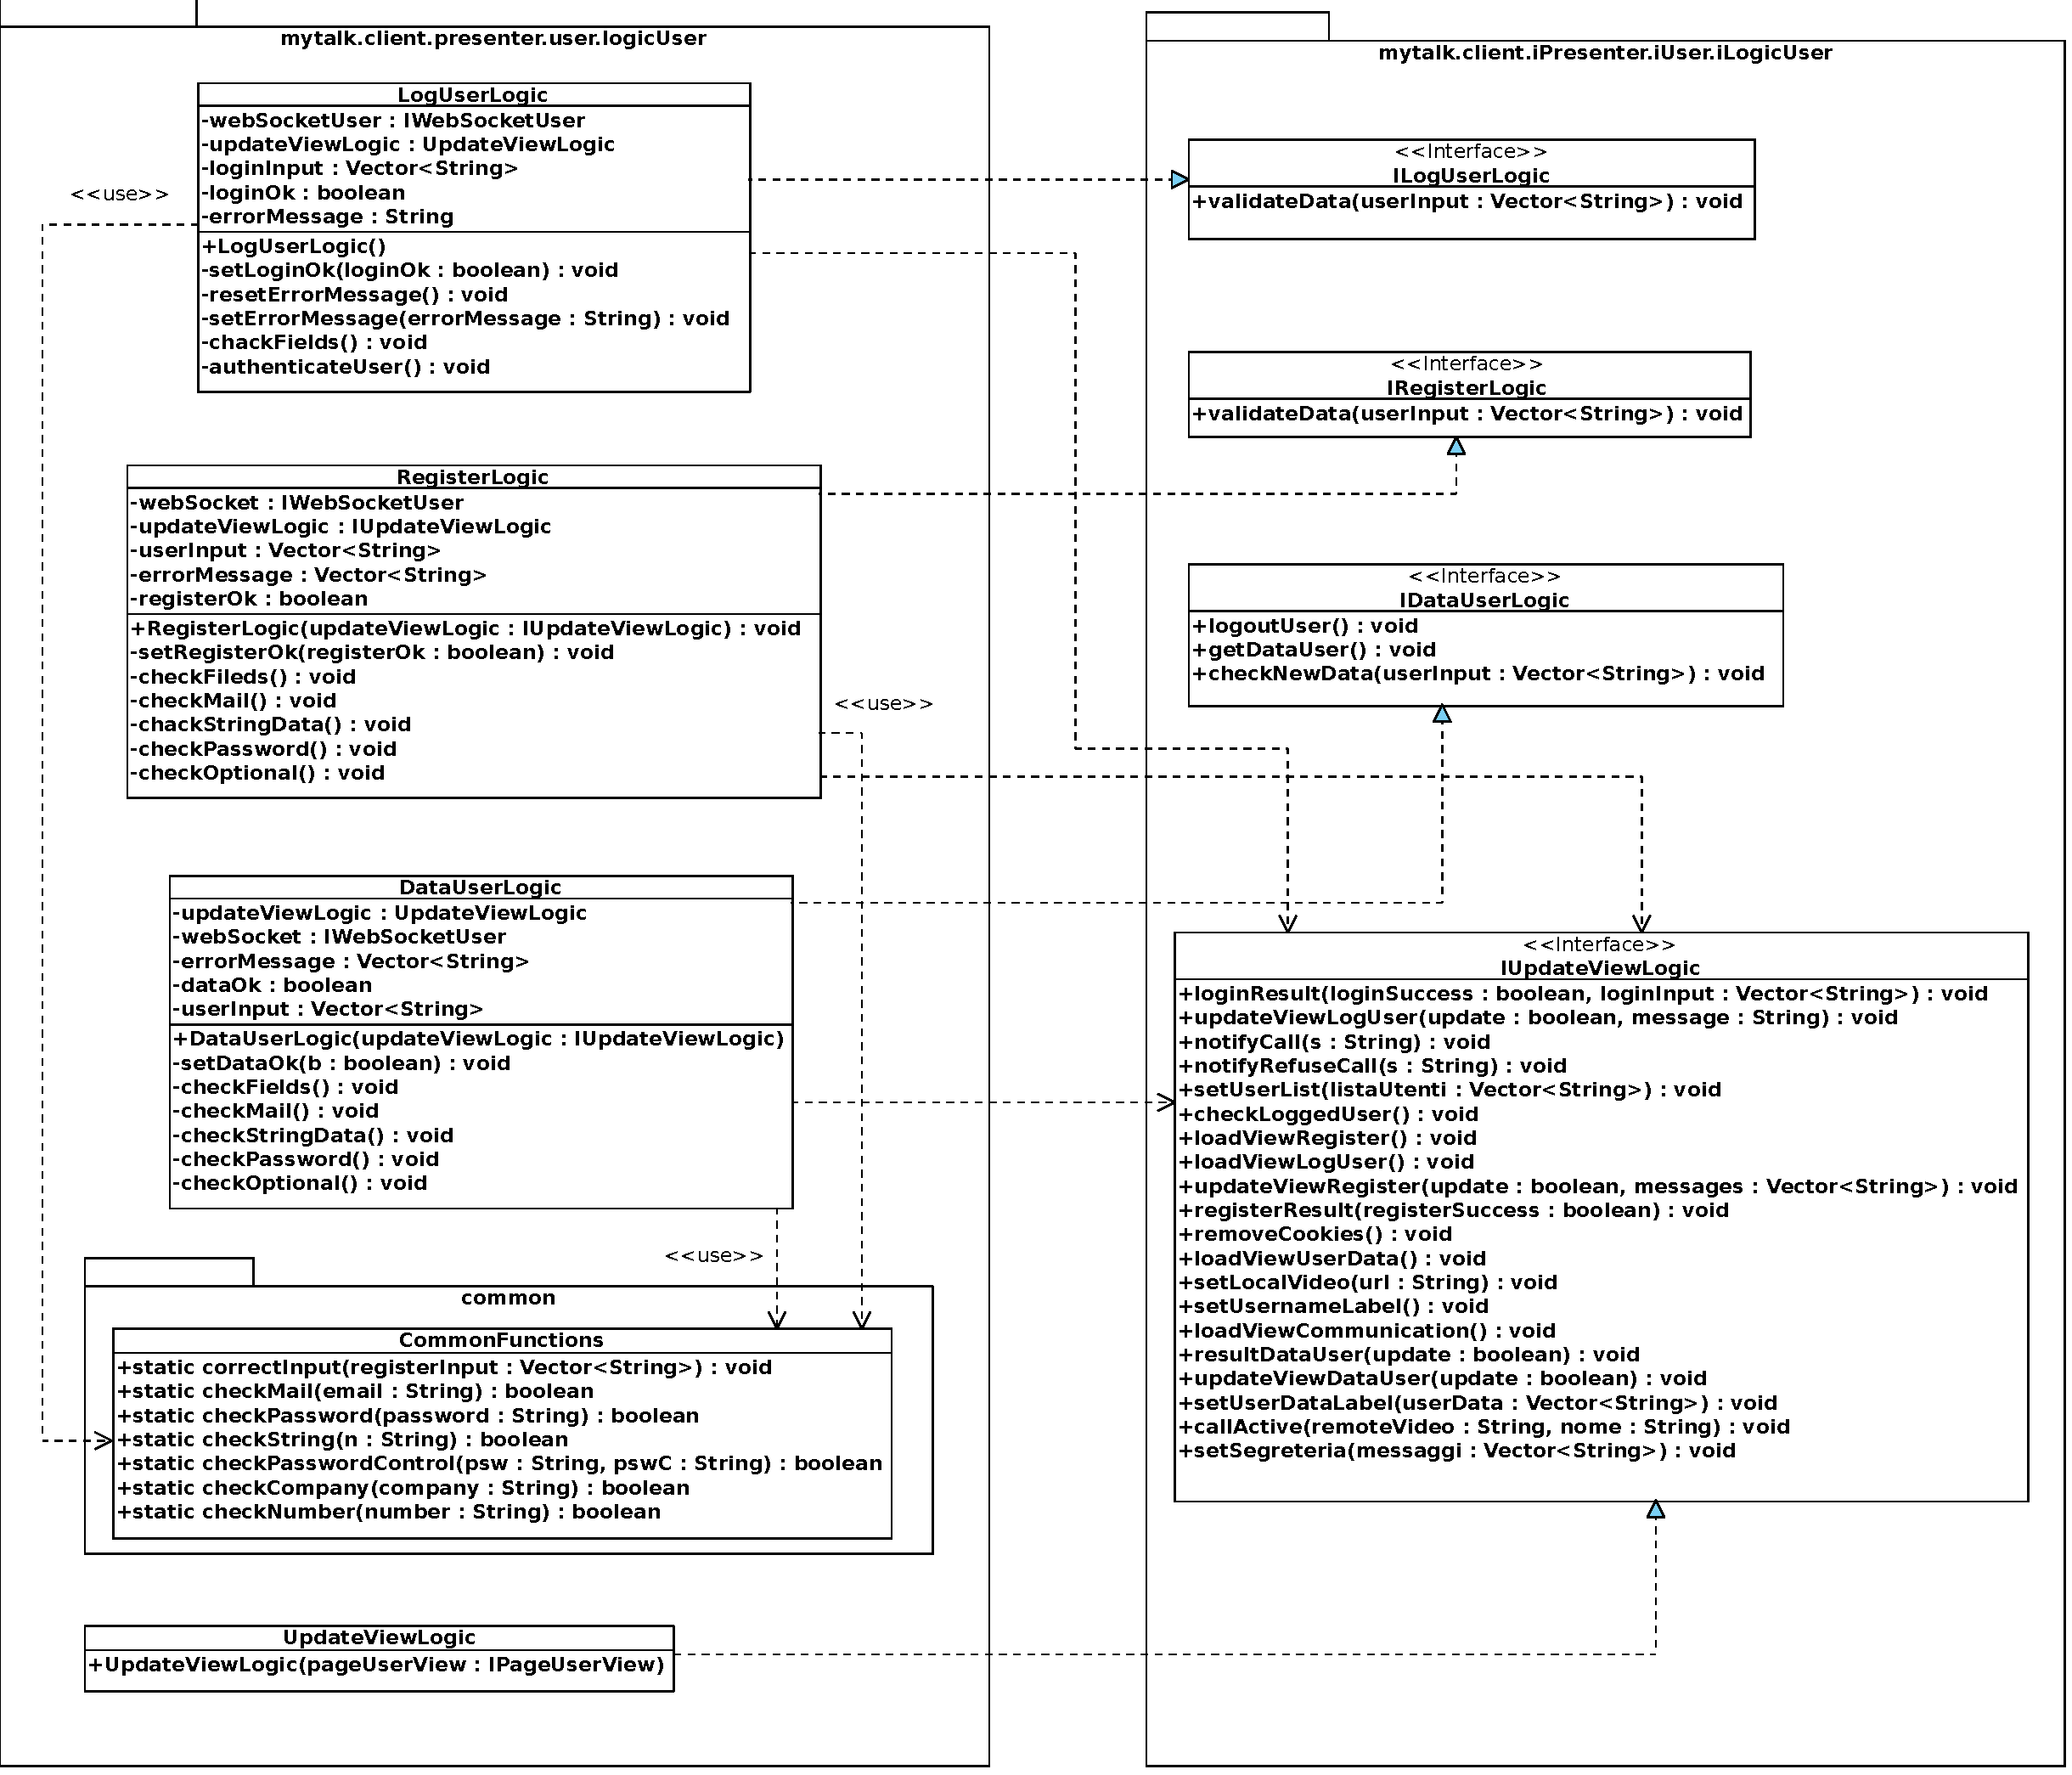
\includegraphics[scale=0.43]{\docsImg classi/presenterLogicUser.pdf}
\caption{Diagramma delle classi dei package \nolinkurl{mytalk.client.iPresenter.iUser.iLogicUser} e  \nolinkurl{mytalk.client.presenter.user.logicUser}; dettaglio delle classi \nolinkurl{ILogUserLogic}, \nolinkurl{IRegisterLogic}, \nolinkurl{IDataUserLogic}, \nolinkurl{IUpdateViewLogic}, \nolinkurl{LogUserLogic}, \nolinkurl{RegisterLogic}, \nolinkurl{DataUserLogic}, \nolinkurl{IUpdateViewLogic} e \nolinkurl{mytalk.client.presenter.user.logicUser.common.CommonFunctions}.}		
	\end{figure}
	
	\begin{figure}[h!tbp]
		\centering
		\label{fig:presenterCommunicationLogicUser}
		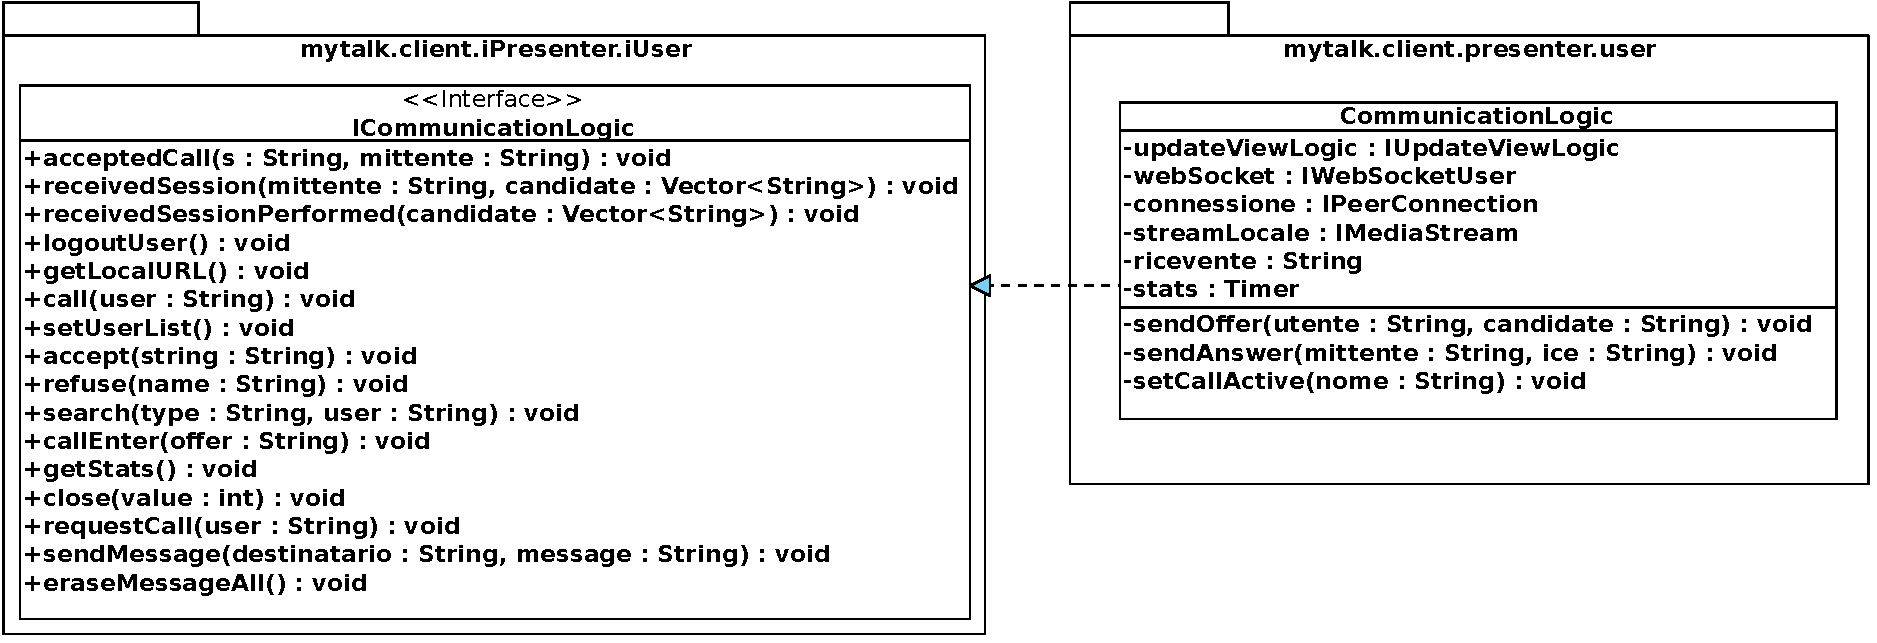
\includegraphics[scale=0.55]{\docsImg classi/presenterCommunicationLogic.pdf}
\caption{Diagramma delle classi dei package \nolinkurl{mytalk.client.iPresenter.iUser} e  \nolinkurl{mytalk.client.presenter.user}; dettaglio delle classi \nolinkurl{ICommunicationLogic} e \nolinkurl{CommunicationLogic}.}		
	\end{figure}	
	
	
					% ICommunicationLogic - inizio
			\paragraph{ICommunicationLogic}\label{par:ICommunicationLogic}{
			\begin{itemize}
				\item[] \textbf{Funzione:}\\
					Interfaccia che offre le operazioni alle classi che hanno il compito di comporre gli oggetti che serviranno per instaurare una nuova comunicazione, chiudere una comunicazione in atto, gestire le comunicazioni in ingresso e gestire l'accesso ai media locali e remoti.\\
				
				\item[] \textbf{Relazioni con altre componenti:}\\
					L'interfaccia è implementata da:
					\begin{itemize}
						\item[]	\path{mytalk.client.presenter.user.logicUser.CommunicationLogic}.
					\end{itemize} 
					L'interfaccia è utilizzata da:
					\begin{itemize}
						\item[] \path{mytalk.client.presenter.user.serverComUser.WebSocketUser}.\\
					\end{itemize}
			
				\item[] \textbf{Metodi:}\\
					\texttt{+ void call(String utente);}\\
					Effettua una chiamata verso l'utente identificato dalla stringa \texttt{utente}. \\
					
					\texttt{+ void accept(String utente);} \\ 
					Accetta la chiamata effettuata dall'utente identificato dalla stringa \texttt{utente}.\\ 
					
					\texttt{+ void callEnter(String offer);}\\
					Crea una descrizione della sessione locale rispetto alla descrizione di una sessione remota passata come parametro.\\

					\texttt{+ void close(int voto);}\\
					Invia un segnale che indica di terminare la chiamata. Il parametro passato come riferimento indica l'opinione data dall'utente al servizio.\\
					
					\texttt{+ String getLocalURL();}\\
					Restituisce l'URL\g~ associato allo stream\g~ locale.\\

					\texttt{+ void getStats();}\\
					Recupera le statistiche prelevate all'ultimo campionamento.\\

					\texttt{+ void refuse(String utente);} \\
					Rifiuta la chiamata dall'utente identificato dalla stringa \texttt{utente}.\\  
					
					\texttt{+ void acceptedCall(String answer, String utente);} \\
					Notifica una chiamata accettata dall'utente \texttt{utente} e che quindi è stata precedentemente inviata.\\
		
					\texttt{+ void receivedSessionPerformed(String mittente, Vector<String> iceCandiate}\\
					Viene richiamato quando è stata effettuata una chiamata e questa è stata accettata dall'altro utente. Tale metodo permette di conoscere l'utente che ha inviato la descrizione e gli \texttt{IceCandidate} inviati in risposta.\\
			
					\texttt{+ void receivedSession(String mittente, Vector<String> candidate);}\\
					Permette di ricevere dei \texttt{candidate} e di gestirli in seguito alla ricezione di una comunicazione.\\

					\texttt{+ void logoutUser();}\\
					Permette all'utente di effettuare il logout.\\
					
					\texttt{+ void setUserList();}\\
					Invia al server\g~ la richiesta della lista di utenti registrati al server\g.\\
					
					\texttt{+ void search(String type, String user);}\\
					Invia al server una richiesta riguardante l'esistenza di un utente registrato al servizio.\\

					\texttt{+ void setUserList();}\\
					Richiede al server\g, tramite \texttt{WebSocket}, la lista degli utenti registrati al servizio.\\
					
					\texttt{+ void setUsernameLabel();}\\
					Imposta la label del nome dell'utente autenticato.\\
					
					\texttt{+ void loadViewUserData();}\\
					Richiama la GUI\g~ relativa alla gestione dei dati.\\
					
					\texttt{+ void logoutUser();}\\
					Effettua il logout dell'utente.\\
					
					\texttt{+ void sendMessage(String destinatario, String message);}\\
					Invia un messaggio all'utente indicato dalla stringa \texttt{destinatario}.\\
					 
					\texttt{+ void eraseMessageAll();}\\
					Elimina tutti i messaggi della casella di posta dell'utente.\\	
			\end{itemize}
			}
			% ICommunicationLogic - fine
		

			% IDataUserLogic - inizio
			\paragraph{IDataUserLogic}\label{par:IDataUserLogic}{
			\begin{itemize}
			
				\item[] \textbf{Funzione:}\\
					Interfaccia che rappresenta l'accesso agli oggetti che gestiscono il recupero e la modifica dei dati personali dell'utente, verificandone la conformità e inoltrando le richieste di modifica alla componente dedita alla comunicazione con il server\g.\\
			
				\item[] \textbf{Relazioni con altre componenti:}{\\
				L'interfaccia è implementata da:
				\begin{itemize}
				 	\item[]	\path{mytalk.client.presenter.user.logicUser.DataUserLogic}.
				\end{itemize}
				L'interfaccia è utilizzata da:
				\begin{itemize}
					\item[] \path{mytalk.client.presenter.user.serverComUser.WebSocketUser};
					\item[] \path{mytalk.client.view.user.LogUser}.\\
				\end{itemize}
				}
			
				\item[] \textbf{Metodi:}{\\
					\texttt{+ void logoutUser();}\\
					Effettua il logout dell'utente.\\
					
					\texttt{- void getDataUser();}\\
					Richiama il metodo \texttt{getUserData} di \texttt{WebSocketUser} che recupera tutti i dati dell'utente.\\
					
					\texttt{- void checkNewData(Vector<String> userInput);}\\
					Controlla i dati inseriti dall'utente.\\
					
					\texttt{+ void loadViewCommunication();}\\
					Richiama la GUI\g~ relativa alla comunicazione.\\
				}
			\end{itemize}
			}
			% IDataUserLogic - fine
		

			% ILogUserLogic - inizio
			\paragraph{ILogUserLogic}\label{par:ILogUserLogic}{
			\begin{itemize}
				\item[] \textbf{Funzione:}\\
				Interfaccia che rappresenta l'accesso alle classi logiche che hanno il compito di gestire il login e logout dell'utente al servizio.\\
			
				\item[] \textbf{Relazioni con altre componenti:}\\
				L'interfaccia è implementata da:
				\begin{itemize}
				 	\item[]	\path{mytalk.client.presenter.user.logicUser.LogUserLogic}.
				\end{itemize}	
				L'interfaccia è utilizzata da:
				\begin{itemize}
					\item[] \path{mytalk.client.view.user.LogUser}.\\
				\end{itemize}
			
				\item[] \textbf{Metodi:}{\\
					\texttt{+ void validateData(Vector<String> userInput);} \\
					Memorizza l'input dell'utente nel campo dati \texttt{loginInput} e richiama il metodo \texttt{checkFields()} per controllare i dati inseriti dall'utente. Invoca il metodo \texttt{resetErrorMessage()} per resettare il messaggio di errore se ripetuto più volte.\\
					
					\texttt{+ void loadViewRegister();}\\
					Richiama la GUI\g~ relativa alla registrazione.\\
				}
			\end{itemize}
			}
			% ILogUserLogic - fine
			
		

			% IRegisterLogic - inizio
			\paragraph{IRegisterLogic}\label{par:IRegisterLogic}{
			\begin{itemize}
			
				\item[] \textbf{Funzione:}\\
				Interfaccia che rappresenta l'accesso alle classi logiche che hanno il compito di gestire i dati di registrazione inseriti dall'utente nella View.\\
			
				\item[] \textbf{Relazioni con altre componenti:}{\\
				L'interfaccia è implementata da:
				\begin{itemize}
				 	\item[] \path{mytalk.client.presenter.user.logicUser.RegisterLogic}.
				\end{itemize}
				L'interfaccia è utilizzata da:
				\begin{itemize}
					\item[] \path{mytalk.client.presenter.user.logicUser.Register}.\\
				\end{itemize}
				}
			
				\item[] \textbf{Metodi:}{\\
					\texttt{+ void validateData(Vector<String> userInput);}\\
					Memorizza l'input dell'utente nel campo dati \texttt{loginInput} e richiama il metodo \texttt{checkFields()} per controllare i dati inseriti dall'utente. Invoca il metodo \texttt{resetErrorMessage()} per resettare il messaggio di errore in caso di errori ripetuti.\\
					
					\texttt{+ void loadViewLogUser();}\\
					Richiama la GUI\g~ relativa all'autenticazione dell'utente.\\
				}
			\end{itemize}
			}
			% IRegisterLogic - fine
		

			% IUpdateViewLogic - inizio
			\paragraph{IUpdateViewLogic}\label{par:IUpdateViewLogic}{
			\begin{itemize}
			
				\item[] \textbf{Funzione:}\\
				Interfaccia che offre i metodi da inoltrare alla view in seguito agli aggiornamenti effettuati dal presenter.\\
			
				\item[] \textbf{Relazioni con altre componenti:}\\
				L'interfaccia è implementata da:
				\begin{itemize}
				 	\item[]	\path{mytalk.client.presenter.user.logicUser.UpdateViewLogic}.
				\end{itemize}
				L'interfaccia è utilizzata da:
				\begin{itemize}
					\item[] \path{mytalk.client.presenter.user.logicUser.CommunicationLogic};
					\item[] \path{mytalk.client.presenter.user.logicUser.DataUserLogic};
					\item[] \path{mytalk.client.presenter.user.logicUser.LogUserLogic};
					\item[] \path{mytalk.client.presenter.user.logicUser.RegisterLogic};
					\item[] \path{mytalk.client.presenter.user.serverComUser.WebSocketUser}.\\
				\end{itemize}
			
				\item[] \textbf{Metodi:}{\\
					\texttt{+void loginResult(boolean loginSucces, Vector<String> loginInput);}\\
					Crea il cookie\g~ di sessione contenente il nome dell'utente, 
					altrimenti imposta un opportuno messaggio di errore.
					Successivamente, aggiorna la View di conseguenza.\\

					\texttt{+ void updateViewLogUser(boolean update, String message);}\\
					Richiama il metodo \texttt{updateViewLogUser} della classe \texttt{PageUserView}.\\

					\texttt{+void notifyCall(String utente);}\\
					Richiama il metodo \texttt{notifyExternalCall} della classe \texttt{PageUserView} al fine di informare l'utente che vi è una chiamata in entrata.\\

					\texttt{+ void notifyRefuseCall(String utente);}\\
					Richiama il metodo \texttt{notifyRefuseCall} della classe \texttt{PageUserView} al fine di informare l'utente che la sua chiamata è stata rifiutata.\\

					\texttt{+ void setUserList(Vector<String> listaUtenti);}\\
					Richiama il metodo \texttt{setUsersList} della classe \texttt{PageUserView} al fine di impostare la lista degli utenti registrati al servizio.\\
					
					\texttt{+ void checkLoggedUser();}\\
					Controlla che l'utente sia autenticato.\\
					
					\texttt{+ void loadViewRegister();}\\
					Richiama il metodo \texttt{loadViewRegister} della classe \texttt{PageUserView} al fine di caricare la schermata per la registrazione di un nuovo utente.\\
					
					\texttt{+ void loadViewLogUser();}\\
					Richiama il metodo \texttt{loadViewLogUser} della classe \texttt{PageUserView} al fine di caricare la schermata per il login dell'utente.\\
					
					\texttt{+ void updateViewRegister(boolean update, Vector<String> messages);}\\
					Richiama il metodo \texttt{updateViewRegister} della classe \texttt{PageUserView} al fine di informare l'utente sull'esito negativo e sui relativi errori della registrazione al servizio precedentemente inviata.\\
					
					\texttt{+ void registerResult(boolean registerSuccess);}\\
					Riceve l'esito della registrazione.\\

					\texttt{+ void removeCookies();}\\
					Rimuovere il cookie\g~ relativo alla sessione corrente.\\

					\texttt{+ void loadViewUserData();}\\
					Richiama il metodo \texttt{loadViewUserData} della classe \texttt{PageUserView} al fine di caricare la schermata che permette all'utente di gestire i propri dati personali.\\
					
					\texttt{+ void setLocalVideo(String url);}\\
					Richiama il metodo \texttt{setLocalVideo} della classe PageUserView per visualizzare il video locale all'interno della pagina HTML\g.\\

					\texttt{+ void setUsernameLabel();}\\
					Richiama il metodo \texttt{setUsernameLabel} della classe \texttt{PageUserView}. Passandogli il nome utente recuperato dal cookie\g~ di sessione.\\
					
					\texttt{+ void loadViewCommunication();}\\
					Richiama il metodo \texttt{loadViewCommunication} della classe \texttt{PageUserView} per caricare la schermata che permette all'utente di inviare e ricevere comunicazioni\\.

					\texttt{+ void resultDataUser(boolean update);}\\
					Riceve l'esito della modifica dei dati e richiama il metodo
					\texttt{updateViewDataUser} passandogli l'esito e il vector contenente i messaggi d'errore.\\
					
					\texttt{+ void updateViewDataUser(boolean update, Vector<String> messages);}\\
					Il metodo ha lo scopo di aggiornare la schermata dell'utente con il risultato della precedente richiesta di modifica dei dati. Per far ciò richiama il metodo \texttt{updateViewDataUser} della classe \texttt{PageUserView}, dopo aver richiamato il metodo \texttt{setUsernameLabel}.\\
					
					\texttt{+ void setUserDataLabel(Vector<String> userData);}\\
					Richiama il metodo \texttt{setUserDataLabel} della classe \texttt{PageUserView} per impostare nell'interfaccia grafica il nome dell'utente attualmente connesso.\\
					
					\texttt{+ void callActive(String remoteVideo, String nome);}\\
					Il metodo ha lo scopo di impostare l'url dello stream condiviso dall'utente remoto, in modo da visualizzarlo all'interno della pagina HTML\g, il metodo inoltre imposta la label che mostra all'utente lo username dell'utente con cui si sta comunicando. Il metodo richiama il metodo \texttt{callActive} della classe \texttt{PageUserView}.\\
					
					\texttt{+ void updateFormInfoChiamata(Vector<Double> dataCall);}\\
					Richiama l'aggiornamento della GUI\g~ del pannello di visualizzazione delle statistiche con i dai passati come parametro.\\
					
					\texttt{+ void updatePanelSearch(boolean b, String user);}\\
					Aggiorna il pannello di ricerca dell’utente tramite nome utente o indirizzo IP\g.\\
					
					\texttt{+ void setSegreteria(Vector<String> messaggi);}\\
					Richiama il metodo dell'oggetto \texttt{pageUserView void setSegreteria(Vector<String> messaggi)} al fine di permettere la visualizzazione nell'interfaccia grafica dei messaggi in segreteria.\\
				}
			\end{itemize}
			}
			% IUpdateViewLogic - fine
	
	}
	
	
	\subsubsection{Package mytalk.client.presenter.user.logicUser}{
	
			% CommunicationLogic - inizio
			\paragraph{CommunicationLogic}\label{par:CommunicationLogic}{
			\begin{itemize}
				\item[] \textbf{Funzione:}\\
				 La classe permette di effettuare e ricevere chiamate e gestione degli stream\g~ audio e video. Comunica con il Model e aggiorna opportunamente la View visualizzando messaggi per l'utente ed aggiornando gli stream\g. \\
			
			\item[] \textbf{Relazioni con altre componenti:}\\			
				implementa l'interfaccia: 
					\begin{itemize}
						\item[] \path{mytalk.client.iPresenter.iUser.iLogicUser.ICommunicationLogic}.
					\end{itemize}
				Usa le classi:
					\begin{itemize}
				 		\item[] \path{mytalk.client.presenter.user.serverComUser.WebSocketUser};
				 		\item[]
\path{mytalk.client.presenter.user.logicUser.UpdateViewLogic}.
				 	\end{itemize}
				tramite le interfacce:
				 	\begin{itemize}
\item[]\path{mytalk.client.iPresenter.iUser.iLogicUser.IUpdateViewLogic}; 		\item[]\path{mytalk.client.iPresenter.iUser.iServerComUser.IWebSocketUser}.\\
					\end{itemize}
				
				\item[] \textbf{Attributi:}\\
					\texttt{- IUpdateViewLogic updateView}: riferimento alla classe \texttt{UpdateViewLogic} che permette di inviare richieste di aggiornamento dell'interfaccia grafica. \\

					\texttt{- IWebSocketUser webSocket}: riferimento alla classe \texttt{WebSocketUser} che permette di inviare comunicazioni al server\g~ tramite l'interfaccia \texttt{IWebSocketUser}.\\

					\texttt{- IPeerConnection connessione}: rifermento alla classe \texttt{PeerConnection} che permette di instaurare, gestire e chiudere una comunicazione.\\

					\texttt{- IMediaStream streamLocale}: riferimento alla classe \texttt{MediaStream} che permette di richiedere l'accesso alla videocamera dell'utente e di convertire l'oggetto ottenuto in un'URL\g~ visualizzabile in una pagina web\g~.\\

					\texttt{- String Ricevente}: riferimento ad un oggetto stringa che ha il compito di memorizzare il nome utente di un utente con cui si sta comunicando.\\
	
					\texttt{- Timer stats}: riferimento ad un oggetto di tipo \texttt{Timer} che serve a campionare le statistiche in maniera ripetuta e di inviarle all'interfaccia grafica.\\

				\item[] \textbf{Metodi:}{\\
					\texttt{+ CommunicationLogic(IPageUserView v, IWebSocketUser w);}\\
					Inizializza il campo dati connessione degli oggetti \texttt{updateView} e \texttt{webSocket}, inizializza gli oggetti \texttt{connessione} e \texttt{streamLocale} tramite i rispettivi costruttori di default e inizializza l'oggetto \texttt{statis} di tipo \texttt{Timer}.\\

					\texttt{+ void call(String utente);}\\
					Viene richiamato quando un utente ne vuole richiamare un altro. Per effettuare la chiamata richiama il metodo dell'oggetto \texttt{WebSocketUser call(String utente, String offer)}, passandogli come parametri il nome utente e la descrizione della sessione locale (che è di tipo \texttt{offer}). La descrizione della sessione locale viene creata invocando il metodo della classe \texttt{PeerConnection inizialize()} e viene reperita già serializzata in formato JSON invocando il metodo della classe \texttt{PeerConnection getOffer()}.\\
 La descrizione della sessione locale è un oggetto delle \texttt{API WebRTC} che contiene informazione riguardanti i media condivisi e il protocollo utilizzato per stabilire la connessione peer-to-peer (nel caso delle WebRTC\g~ è il protocollo ICE).\\
 
					\texttt{+ void accept(String utente);}\\
					Viene richiamato quando si vuole accettare una chiamata da parte dell'utente identificato dalla stringa \texttt{"utente"} passata come parametro attuale. Vi è quindi stata in precedenza una chiamata ricevuta da parte dell'utente passato come parametro e questa chiamata è stata accettata.\\
					Il metodo, per segnalare al server\g~ e all'utente l'accettazione della chiamata, richiama il metodo \texttt{accept(String utente, String answer)} dell'oggetto \texttt{Socket} di tipo \texttt{WebSocketUser}, passandogli come parametri, oltre al nome dell'utente che ha chiamato, anche la descrizione locale (che sarà di tipo \texttt{answer}) estratta tramite l'invocazione del metodo \texttt{getAnswer()} della classe \texttt{PeerConnection}.\\
					La descrizione della sessione locale è un oggetto delle \texttt{API WebRTC} che contiene informazione riguardanti i media condivisi e il protocollo utilizzato per stabilire la connessione peer-to-peer (nel caso delle WebRTC\g~ è il protocollo ICE).\\

					\texttt{+ String getLocalURL();}\\
					Restituisce l'URL\g~ associato allo stream\g~ locale. Per ottenere tale URL\g~ il metodo richiama il metodo \texttt{localURL} dell'oggetto \texttt{StreamLocale}.\\

					\texttt{+ void close(int value);}\\
					Chiude eventuali comunicazioni in atto. Per chiudere la comunicazione richiama il metodo dell'oggetto \texttt{connessione} \texttt{close()}. Prima di richiamarlo invia le statistiche al server\g~ attraverso il metodo dell'oggetto \texttt{Socket sendStats(String ricevente, vector<Double> statistiche)}.\\

					\texttt{+ void refuse(String utente);}\\
					Viene richiamato quando si vuole rifiutare una chiamata da parte dell'utente identificato dalla stringa \texttt{utente} passata come parametro attuale.
					Per segnalare al server\g~ e all'utente il rifiuto della chiamata viene richiamato il metodo \texttt{refuse(String utente)} dell'oggetto \texttt{Socket} di tipo \texttt{WebSocketUser}.\\

					\texttt{+ void getStats();}\\
					Quando viene richiamato invia alla View le statistiche estrapolate dall'oggetto \texttt{Connessione} richiamando il metodo \texttt{getStats()}. Per inviare le statistiche alla GUI\g~ viene richiamato il metodo \texttt{updateFormInfoChiamata(Vector<Double> statistiche)} dell'oggetto \texttt{updateViewLogic}\\.

					\texttt{+ void acceptedCall(String answer, String utente);}\\
					Notifica alla classe che la chiamata dall'altro lato della comunicazione è stato accettata e che si può procedere con l'impostazione della sessione remota, passata come parametro in formato JSON\g~.\\
					Il metodo assegna al campo dati \texttt{Ricevente} il valore della stringa passata come parametro al metodo, imposta la descrizione remota richiamando il metodo \texttt{setRemoteAnswer(String answer)}, recupera gli \texttt{IceCandidate} dall'oggetto \texttt{connessione} tramite il metodo \texttt{getCandidates()}. Invia l'utente identificato dal parametro formale \texttt{utente} tramite \texttt{WebSocket} al server\g~ richiamando il metodo \texttt{sendOffer(String utente, String candidati)}.\\

					\texttt{- void sendOffer(String utente, String candidati);}\\
					Invia gli \texttt{IceCandidate} di comunicazione costituiti da oggetti \texttt{RTCICeCandidate} all'oggetto \texttt{Socket} che poi provvederà ad inviarlo al server\g.\\
					Il metodo richiama il metodo dell'oggetto \texttt{Socket sendOffer(utente, candidati)} che poi provvederà ad inviare gli \texttt{IceCandidate} codificati in formato JSON\g al server\g, il quale girerà poi il messaggio all'utente ricevente.\\

					\texttt{- void sendAnswer(String mittente, String candidate);}\\
					Invia gli \texttt{IceCandidate} di comunicazione costituiti da oggetti \texttt{RTCIceCandidate} all'oggetto \texttt{Socket} che poi provvederà ad inviarlo al server\g.\\
					Viene richiamato il metodo dell'oggetto \texttt{Socket} \texttt{sendAnswer(utente, candidati)} che provvederà ad inviare gli \texttt{IceCandidate} codificati in formato JSON\g~ al server\g, il quale girerà poi il messaggio all'utente ricevente.\\

					\texttt{+ void receivedSessionPerformed(Vector<String> candidate);}\\
					Imposta la descrizione di sessione remota di tipo \texttt{answer} giunta tramite il \texttt{WebSocket}, in modo che sia possibile iniziare la comunicazione.\\
					Viene richiamato il metodo dell'oggetto \texttt{Connessione} di tipo \texttt{PeerConnection receivedCommunication(JavaScriptObject description)} per impostare la descrizione di sessione.\\

					\texttt{+ void receivedSession(String mittente, Vector<String> candidate);}\\
					Aggiunge i candidati ICE alla connessione richiamando ripetutamente il metodo della classe \texttt{PeerConnection addCandidate(String candidate)}, successivamente reperisce gli \texttt{IceCandidate} dalla connessione tramite \texttt{PeerConnection getCandidates()} e richiama il metodo \texttt{sendAnswer(String utente, String candidates)} per inviare gli oggetti di tipo \texttt{RTCIceCandidate} in risposta all'utente che ha inviato i suoi candidati in precedenza.\\
	
					\texttt{+ void callEnter(String offer);}\\
					Il metodo ha il compito di richiamare il metodo della classe \texttt{PeerConnection} \texttt{answer(String offer)}, tramite il quale il sistema riesce a creare una descrizione di sessione locale di tipo \texttt{answer} in relazione alla descrizione di sessione remota di tipo \texttt{offer} passata come riferimento al metodo.\\
					
					\texttt{- void setCallActive(String utente);}\\
					Il metodo prima recupera l'URL remoto dalla classe \texttt{PeerConnection} tramite il metodo \texttt{getRemoteURL()}, poi richiama il metodo della classe \texttt{UpdateViewLogic callActive(String url, String utente}, che imposterà lo stream\g~ remoto all'interno dell'interfaccia grafica e imposterà il nome dell'utente con il quale si sta comunicando. Il richiamo di questo metodo dà inizio alla comunicazione vera e propria.\\
					
					\texttt{+ void logoutUser();}\\
					Effettua il logout dell'utente: chiama i metodi per rimuovere il cookie\g~ associato all'utente e aggiornare la View.\\
					
					\texttt{+ void search(String type, String user);}\\
					Invia al server\g~ una richiesta riguardante l'esistenza di un utente registrato al servizio. Se la ricerca di reperimento dell'username avviene tramite IP\g~, viene richiamato il metodo dell'oggetto \texttt{webSocketUser searchUserByIp(String ip)}, se invece la ricerca avviene per inserimento di una e-mail viene richiamato il metodo della classe \texttt{webSocketUser searchUserByEMail(String user)}.\\
					
					\texttt{+ void setUserList();}\\
					Richiede al server\g, tramite \texttt{WebSocket}, la lista degli utenti registrati al servizio.\\
					
					\texttt{+ void setUsernameLabel();}\\
					Imposta la label del nome dell'utente autenticato richiamando il metodo \path{mytalk.client.presenter.administrator.logicUser.UpdateViewLogic.setUsernameLabel()}.\\
					
					\texttt{+ void logoutUser();}\\
					Effettua il logout dell'utente: richiama i metodi per rimuovere il cookie\g~ associato all'utente e aggiornare la View.\\
					
					\texttt{+ void sendMessage(String destinatario, String message);}\\
					Richiamando il metodo dell'oggetto \texttt{webSocketUser sendMessage(String destinatario, String message)} invia un messaggio all'utente indicato dalla stringa \texttt{destinatario}.\\
					 
					\texttt{+ void eraseMessageAll();}\\
					Richiamando il metodo dell'oggetto \texttt{webSocketUser void eraseMessageAll()} elimina tutti i messaggi della casella di posta dell'utente.\\					
					\texttt{+ void loadViewUserData()}\\
					Richiama la GUI\g~ relativa alla gestione dei dati richiamando il metodo \path{mytalk.client.presenter.administrator.logicUser.UpdateViewLogic.loadViewUserData()}.\\
				}
			\end{itemize}
			}
			% CommunicationLogic - fine

		

			% DataUserLogic - inizio
			\paragraph{DataUserLogic}\label{par:DataUserLogic}{
			\begin{itemize}
			
				\item[] \textbf{Funzione:}\\
					La classe controlla che i dati che l'utente vuole modificare siano corretti tramite l'utilizzo di espressioni regolari e richiama opportuni metodi della classe che gestisce i \texttt{WebSocket} per poter modificare in maniera persistente i dati dell'utente autenticato.\\
				
				\item[] \textbf{Relazioni con altre componenti:}{\\
					implementa l'interfaccia: 
					\begin{itemize}
						\item[] \path{mytalk.client.iPresenter.iUser.iLogicUser.IDataUserLogic}.
					\end{itemize}								
					Usa le classi:
					\begin{itemize}
						\item[] \path{mytalk.client.presenter.user.logicUser.UpdateViewLogic};
						\item[] \path{mytalk.client.presenter.user.serverComUser.WebSocketUser};
						\item[] \path{mytalk.client.model.localDataUser.ManageCookies}.
					\end{itemize}
					Tramite le interfacce: 
					\begin{itemize}
						\item[] \path{mytalk.client.iPresenter.iUser.iLogicUser.IUpdateViewLogic};
						\item[] \path{mytalk.client.iPresenter.iUser.iServerComUser.IWebSocketUser}.
					\end{itemize}
				}
				
				\item[] \textbf{Attributi:}\\
				\texttt{- Vector<String> userInput}: contiene i nuovi dati inseriti dall'utente.\\
				
				\texttt{- boolean dataOk}: contiene l'esito dei controlli preliminari sui nuovi dati inseriti.\\
				
				\texttt{- Vector<String> errorMessage}: contiene eventuali messaggi di errori che si sono verificati nei controlli preliminari dei dati inseriti.\\
					\texttt{- WebSocketUser webSocket}: è un riferimento all'oggetto \texttt{WebSocketUser}. Tale riferimento permette di inviare messaggi al server\g.\\
					
					\texttt{- IUpdateViewLogic updateViewLogic}: è un riferimento all'oggetto di tipo \texttt{UpdateViewLogic}. Tale riferimento permette di richiamare metodi che poi andranno a modificare la View per visualizzare informazioni per l'utente.\\

				Informazioni generali sui seguenti metodi: tutte le stringhe prima della loro gestione sono state trattate con il metodo \texttt{trim()} che rimuove gli spazi bianchi all'inizio ed alla fine della stringa.
			
				\item[] \textbf{Metodi:}{\\
					\texttt{+ DataUserLogic(IUpdateViewLogic updateViewLogic, IWebSocketUser webSocket)};\\
					Il costruttore inizializza i campi dati dell'oggetto con i parametri passatigli.\\
					
					\texttt{+ void logoutUser();}\\
					Effettua il logout dell'utente: richiama i metodi per rimuovere il cookie\g~ associato all'utente e aggiornare la View.\\
					
					\texttt{+ void getDataUser();}\\
					Richiama il metodo \texttt{getUserData()} della classe \texttt{WebSocketUser}, il quale recupera tutti i dati dell'utente.\\
					
					\texttt{+ void checkNewData(Vector<String> input)}\\
					Controlla che i dati inseriti dall'utente siano corretti, per eseguire i controlli richiama il metodo \texttt{checkFields()}. In caso affermativo richiama il metodo \texttt{changeDataUser} della classe \texttt{WebSocketUser} per aggiornare i dati dell'utente, altrimenti aggiorna la View degli errori.\\
					
					\texttt{+ void checkFields();}\\
					Imposta il vettore contenente i messaggi di errore relativi ad ogni campo, richiama i metodi per controllare i vari campi ed imposta il campo dati \texttt{loginOk} a \texttt{true} se non vengono riscontrati errori, altrimenti a \texttt{false}. I controlli eseguiti per i vari campi sono:
					\begin{itemize}
						\item l'indirizzo e-mail deve avere un formato appropriato;
						\item il nome e il cognome devono essere stringhe;
						\item il numero di telefono deve essere lungo al massimo 10 caratteri tutti numerici.
					\end{itemize}	
					
					\texttt{- void checkEMail();}\\		
					Richiama il metodo di \texttt{CommonFunctions} per controllare che l'indirizzo e-mail abbia un formato appropriato.\\
	
					\texttt{- void checkStringData();}\\
					Richiama il metodo di \texttt{CommonFunctions} per controllare che il nome e il cognome siano composti da stringhe alfabetiche.\\
	
					\texttt{- void checkPassword();}\\
					Richiama il metodo di \texttt{CommonFunctions} per controllare la password e l'uguaglianza della nuova password e della conferma della password.\\

					\texttt{- void checkOptional();}\\
					Richiama i metodi di \texttt{CommonFunctions} per controllare il nome dell'azienda e il numero telefonico.\\
					
					\texttt{+ void loadViewCommunication();}\\
					Richiama la GUI\g~ relativa alla comunicazione richiamando il metodo \path{mytalk.client.presenter.administrator.logicUser.UpdateViewLogic.loadViewCommunication()}.\\
				}
			\end{itemize}
			}
			% DataUserLogic - fine

		

			% LogUserLogic - inizio
			\paragraph{LogUserLogic}\label{par:LogUserLogic}{
			\begin{itemize}
				\item[] \textbf{Funzione:}\\
					la classe ha  il compito di inoltrare la richiesta di login alla classe \texttt{IWebSocketUser}, che comunica con il server\g. Richiama i metodi di \texttt{IUpdateViewLogic} per notificare la View dell'esito della verifica delle credenziali ed effettua il logout dell'utente distruggendo i dati relativi alla sessione.\\
				
				\item[] \textbf{Relazioni con altre componenti:}\\
					implementa l'interfaccia :
					\begin{itemize}
						\item[] \path{mytalk.client.iPresenter.iUser.iLogicUser.ILogUserLogic}.
					\end{itemize}							
					Usa le classi:
					\begin{itemize}
						\item[] \path{mytalk.client.presenter.user.logicUser.common.CommonFunctions};
						\item[] \path{mytalk.client.presenter.user.serverComUser.WebSocketUser};
						\item[] \path{mytalk.client.presenter.user.logicUser.UpdateViewLogic};
					\end{itemize}
					Tramite le interfacce:
					\begin{itemize}	\item[]\path{mytalk.client.iPresenter.iUser.iServerComUser.IWebSocketUser};\\
												\item[]\path{mytalk.client.iPresenter.iUser.iLogicUser.IUpdateViewLogic}.\\

					\end{itemize}
				
				\item[] \textbf{Attributi:}\\
					\texttt{- Vector<String> loginInput}: contiene i dati inseriti dall'utente provenienti dalla View;\\

					\texttt{- boolean loginOk}: indica se i dati inseriti dall'utente risultano corretti o meno;\\

					\texttt{- String errorMessage} messaggio di errore da ritornare all'utente in caso di problemi nel login;\\

					\texttt{- IWebSocketUser webSocketUser}: riferimento alla classe \texttt{WebSocketUser}. Permette di richiamare i metodi per l'autenticazione e la terminazione della sessione utente;\\

					\texttt{- IUpdateViewLogic updateViewLogic}: riferimento alla classe \texttt{UpdateViewLogic}. Permette di richiamare i metodi di aggiornamento della View.\\
			
				\item[] \textbf{Metodi:}\\
					\texttt{+ LogUserLogic(IUpdateViewLogic updateViewLogic, IWebSocketUser webSocketUser);}\\
					Costruttore. Inizializza \texttt{updateViewLogic} e \texttt{webSocketUser} con i valori ricevuti come parametri, crea un nuovo \texttt{Vector<String>} vuoto per \texttt{loginInput}, inizializza a \texttt{true loginOk} e inizializza \texttt{errorMessage}.\\
				
					\texttt{+ void validateData(Vector<String> userInput);}\\
					Memorizza l'input dell'utente in \texttt{loginInput}, richiama il metodo di \texttt{CommonFunctions CorrectInput} e richiama \texttt{checkFields} per verificare i dati ricevuti. Se questi sono corretti, richiama \texttt{authicateUser} per autenticare l'utente. Infine, utilizza il riferimento \texttt{updateViewLogic} per notificare la View dell'esito dell'operazione.\\

					\texttt{- void resetErrorMessage();}\\
					Reimposta il messaggio di errore al valore iniziale. Viene richiamato da \texttt{checkFields()} per evitare di mostrare messaggi di errore ripetuti all'utente.\\

					\texttt{- void checkFields();}\\
					Dopo aver reimpostato \texttt{errorMessage} e \texttt{loginOk} ai valori iniziali, utilizza i metodi della classe astratta \texttt{CommonFunctions} per controllare la correttezza sintattica dell'indirizzo e-mail e della password inseriti dall'utente. In caso di errore, aggiorna il messaggio di errore e imposta \texttt{loginOk} a \texttt{false}.\\

					\texttt{- void authicateUser();}\\
					Autenticazione dell'utente. Richiama il metodo di \texttt{webSocketUser} per autenticare l'utente.\\
					
					\texttt{+ void loadViewRegister();}\\
					Richiama la GUI\g~ relativa alla registrazione richiamando il metodo \path{mytalk.client.presenter.administrator.logicUser.UpdateViewLogic.loadViewRegister()}.\\
			\end{itemize}
			}
			% LogUserLogic - fine

		

			% RegisterLogic - inizio
			\paragraph{RegisterLogic}\label{par:RegisterLogic}{
			\begin{itemize}
			
				\item[] \textbf{Funzione:}\\
					La classe ha il compito di inoltrare la richiesta di registrazione alla classe \texttt{IWebSocketUser}, che comunica con il server\g. Richiama inoltre i metodi di \texttt{IUpdateViewLogic} per notificare la View dell'esito della verifica delle credenziali. La classe permette all'utente di effettuare la registrazione per usufruire del servizio.\\
			
				\item[] \textbf{Relazioni con altri metodi:}{\\
				implementa l'interfaccia:
				\begin{itemize}
					\item[] \path{mytalk.client.iPresenter.iUser.iLogicUser.IRegisterLogic}.
				\end{itemize}
				Usa le classi:
				\begin{itemize}
				 	\item[] \path{mytalk.client.presenter.user.logicUser.common.CommonFunctions};
				 	\item[] \path{mytalk.client.presenter.user.serverComUser.WebSocketUser};
				 \end{itemize}
				 tramite l'interfaccia: 
				 \begin{itemize}
				 	\item[]\path{mytalk.client.iPresenter.iUser.iServerComUser.IWebSocketUser}.\\
				\end{itemize}
				}
				
				\item[] \textbf{Attributi:}\\
					\texttt{- Vector<String> userInput}: contiene i dati inseriti dall'utente provenienti dalla View;\\

					\texttt{- boolean loginOk}: indica se i dati inseriti dall'utente risultano corretti o meno;\\

					\texttt{- String errorMessage}: messaggio di errore da ritornare all'utente in caso di problemi nel login;\\

					\texttt{- IWebSocketUser webSocketUser}: riferimento alla classe \texttt{WebSocketUser}. Permette di richiamare i metodi per l'autenticazione e la terminazione della sessione utente;\\

					\texttt{- IUpdateViewLogic updateViewLogic}: riferimento alla classe \texttt{UpdateViewLogic}. Permette di richiamare i metodi di aggiornamento della View.\\
			
				\item[] \textbf{Metodi:}\\
					\texttt{+ RegisterLogic(IUpdateViewLogic updateViewLogic, IWebSocketUser webSocketUser);}\\
					Costruttore. Inizializza \texttt{updateViewLogic} e \texttt{webSocketUser} con i valori ricevuti come parametri, crea un nuovo \texttt{Vector<String>} per \texttt{registerInput} e lo inizializza con la stringa vuota, inizializza \texttt{loginOk} a \texttt{true}.\\

					\texttt{+ void validateData(Vector<String> userInput);}\\
					Memorizza l'input dell'utente in \texttt{registerInput}, richiama il metodo di \texttt{CommonFunctions CorrectInput} e richiama \texttt{checkFields} per verificare i dati ricevuti. Se questi sono corretti, richiama \path{webSocketUser.inserisciUtente(userInput)} per registrare l'utente. Infine, utilizza il riferimento \texttt{updateViewLogic} per notificare la View dell'esito dell'operazione.\\

					\texttt{- void checkFields();}\\	
					Richiama i vari metodi corrispondenti alla registrazione per controllare l'input dell'utente.
				
					\texttt{- void checkEMail();}\\
					Richiama il metodo di \texttt{CommonFunctions} per controllare l'e-mail.\\

					\texttt{- void checkStringData();}\\
					Richiama il metodo di \texttt{CommonFunctions} per controllare il nome e il cognome.\\

					\texttt{- void checkPassword();}\\
					Richiama il metodo di \texttt{CommonFunctions} per controllare la password e l'uguaglianza della nuova password e della conferma della password.\\

					\texttt{- void checkOptional();}\\
					Richiama i metodi di \texttt{CommonFunctions} per controllare il nome dell'azienda e il numero telefonico.\\
					
					\texttt{+ void loadViewLogUser();}\\
					Richiama la GUI\g~ relativa all'autenticazione dell'utente richiamando il metodo \path{mytalk.client.presenter.administrator.logicUser.UpdateViewLogic.loadViewLogUser()}.\\
			\end{itemize}
			}
			% RegisterLogic - fine

		

			% UpdateViewLogic - inizio
			\paragraph{UpdateViewLogic}\label{par:UpdateViewLogic}{
			\begin{itemize}
			
				\item[] \textbf{Funzione:}\\
					Inoltra alla View tutte le richieste di aggiornamento provenienti dal Presenter. Controlla inoltre se l'utente è autenticato e gestisce l'esito delle operazioni di login, registrazione e modifica dati.\\
			
				\item[] \textbf{Relazioni con altre componenti:}\\
					implementa l'interfaccia: 
					\begin{itemize}
						\item[] \path{mytalk.client.iPresenter.iUser.iLogicUser.IUpdateViewLogic}.
					\end{itemize}
					Usa le classi:
					\begin{itemize}
						\item[] \path{mytalk.client.presenter.user.logicUser.common.CommonFunctions};
						\item[] \path{mytalk.client.view.user.PageUserView};
					\end{itemize}
					tramite l'interfaccia:
					\begin{itemize}
						\item[] \path{mytalk.client.iView.iUser.IPageUserView}.\\
					\end{itemize}
				
				\item[] \textbf{Attributi:}\\
					\texttt{- IPageUserView pageUserView}: riferimento alla classe \path{mytalk.client.view.user.PageUserView}. Permette di richiamare i metodi di aggiornamento della View.\\
			
				\item[] \textbf{Metodi:}{\\
					\texttt{+ UpdateViewLogic(IPageUserView pageUserView);}\\
					Costruttore: inizializza il riferimento \texttt{pageUserView} con quello passatogli come parametro.\\
		
					\texttt{+void loginResult(boolean loginSucces, Vector<String> loginInput);}\\
					Se\texttt{loginSuccess} vale \texttt{true} richiama il metodo di \texttt{ManageCookies} per creare il cookie\g~ di sessione contenente il nome dell'utente, altrimenti imposta un opportuno messaggio di errore.
					Successivamente, aggiorna la View di conseguenza.\\

					\texttt{+ void updateViewLogUser(boolean update, String message);}\\
					Richiama il metodo \texttt{updateViewLogUser} della classe \texttt{PageUserView}.\\

					\texttt{+void notifyCall(String s);}\\
					Richiama il metodo \texttt{notifyExternalCall} della classe \texttt{PageUserView}.\\

					\texttt{+ void notifyRefuseCall(String s);}\\
					Richiama il metodo \texttt{notifyRefuseCall} della classe \texttt{PageUserView}.\\

					\texttt{+ void setUserList(Vector<String> listaUtenti);}\\
					Richiama il metodo \texttt{setUsersList} della classe \texttt{PageUserView}.\\
					
					\texttt{+ void checkLoggedUser();}\\
					Controlla che l'utente sia autenticato. Per farlo prova a recuperare il cookie\g~ di sessione richiamando l'apposito metodo della classe \texttt{ManageCookies}: se il cookie\g~ esiste, l'utente è autenticato.\\
					
					\texttt{+ void loadViewRegister();}\\
					Richiama il metodo \texttt{loadViewRegister} della classe \texttt{PageUserView}.\\
					
					\texttt{+ void loadViewLogUser();}\\
					Richiama il metodo \texttt{loadViewLogUser} della classe \texttt{PageUserView}.\\
					
					\texttt{+ void updateViewRegister(boolean update, Vector<String> messages);}\\
					Richiama il metodo \texttt{updateViewRegister} della classe \texttt{PageUserView}.\\
					
					\texttt{+ void registerResult(boolean registerSuccess);}\\
					Riceve l'esito della registrazione e richiama il metodo \texttt{updateViewRegister} con parametro \texttt{true} o \texttt{false}. Imposta opportunamente il vettore dei messaggi di errore \texttt{messages}.\\

					\texttt{+ void removeCookies();}\\
					Richiama il metodo \texttt{deleteCookies} della classe \texttt{ManageCookies} per rimuovere il cookie\g~ relativo alla sessione corrente.\\

					\texttt{+ void loadViewUserData();}\\
					Richiama il metodo \texttt{loadViewUserData} della classe \texttt{PageUserView}.\\
					
					\texttt{+ void setLocalVideo(String url);}\\
					Richiama il metodo \texttt{setLocalVideo} della classe PageUserView.\\

					\texttt{+ void setUsernameLabel();}\\
					Richiama il metodo \texttt{setUsernameLabel} della classe \texttt{PageUserView}. Gli passa il nome utente recuperato dal cookie\g~ di sessione.\\
					
					\texttt{+ void loadViewCommunication();}\\
					Richiama il metodo \texttt{loadViewCommunication} della classe \texttt{PageUserView}.\\

					\texttt{+ void resultDataUser(boolean update);}\\
					Riceve l'esito della modifica dei dati e richiama il metodo \texttt{updateViewDataUser} passandogli l'esito e il \texttt{Vector} contenente i messaggi d'errore.\\
					
					\texttt{+ void updateViewDataUser(boolean update, Vector<String> messages);}\\
					Richiama il metodo \texttt{updateViewDataUser} della classe \texttt{PageUserView}, dopo aver richiamato il metodo \texttt{setUsernameLabel}.\\
					
					\texttt{+ void setUserDataLabel(Vector<String> userData);}\\
					Richiama il metodo \texttt{setUserDataLabel} della classe \texttt{PageUserView}.\\
					
					\texttt{+ void callActive(String remoteVideo, String nome);}\\
					Richiama il metodo \texttt{callActive} della classe \texttt{PageUserView}.\\
					
					\texttt{+ void updateFormInfoChiamata(Vector<Double> dataCall);}\\
					Richiama il metodo \texttt{updateFormoInfoChiamata(dataCall)} attraverso il riferimento \texttt{pageUserView}.\\
					
					\texttt{+ void updatePanelSearch(boolean b, String user);}\\
					Richiama il metodo \texttt{updatePanelSearch(b, user)} attraverso il riferimento \texttt{pageUserView}.\\
					
					\texttt{+ void setSegreteria(Vector<String> messaggi);}\\
					Richiama il metodo dell'oggetto \texttt{pageUserView void setSegreteria(Vector<String> messaggi)} al fine di permettere la visualizzazione nell'interfaccia grafica dei messaggi in segreteria.\\
				}
			\end{itemize}
			}
			% UpdateViewLogic - fine
		}
	
\newpage	
	
	\subsubsection{Package mytalk.client.iPresenter.iUser.iCommunication}	{
	
	\begin{figure}[h!tbp]
		\centering
		\label{fig:presenterCommunication}
		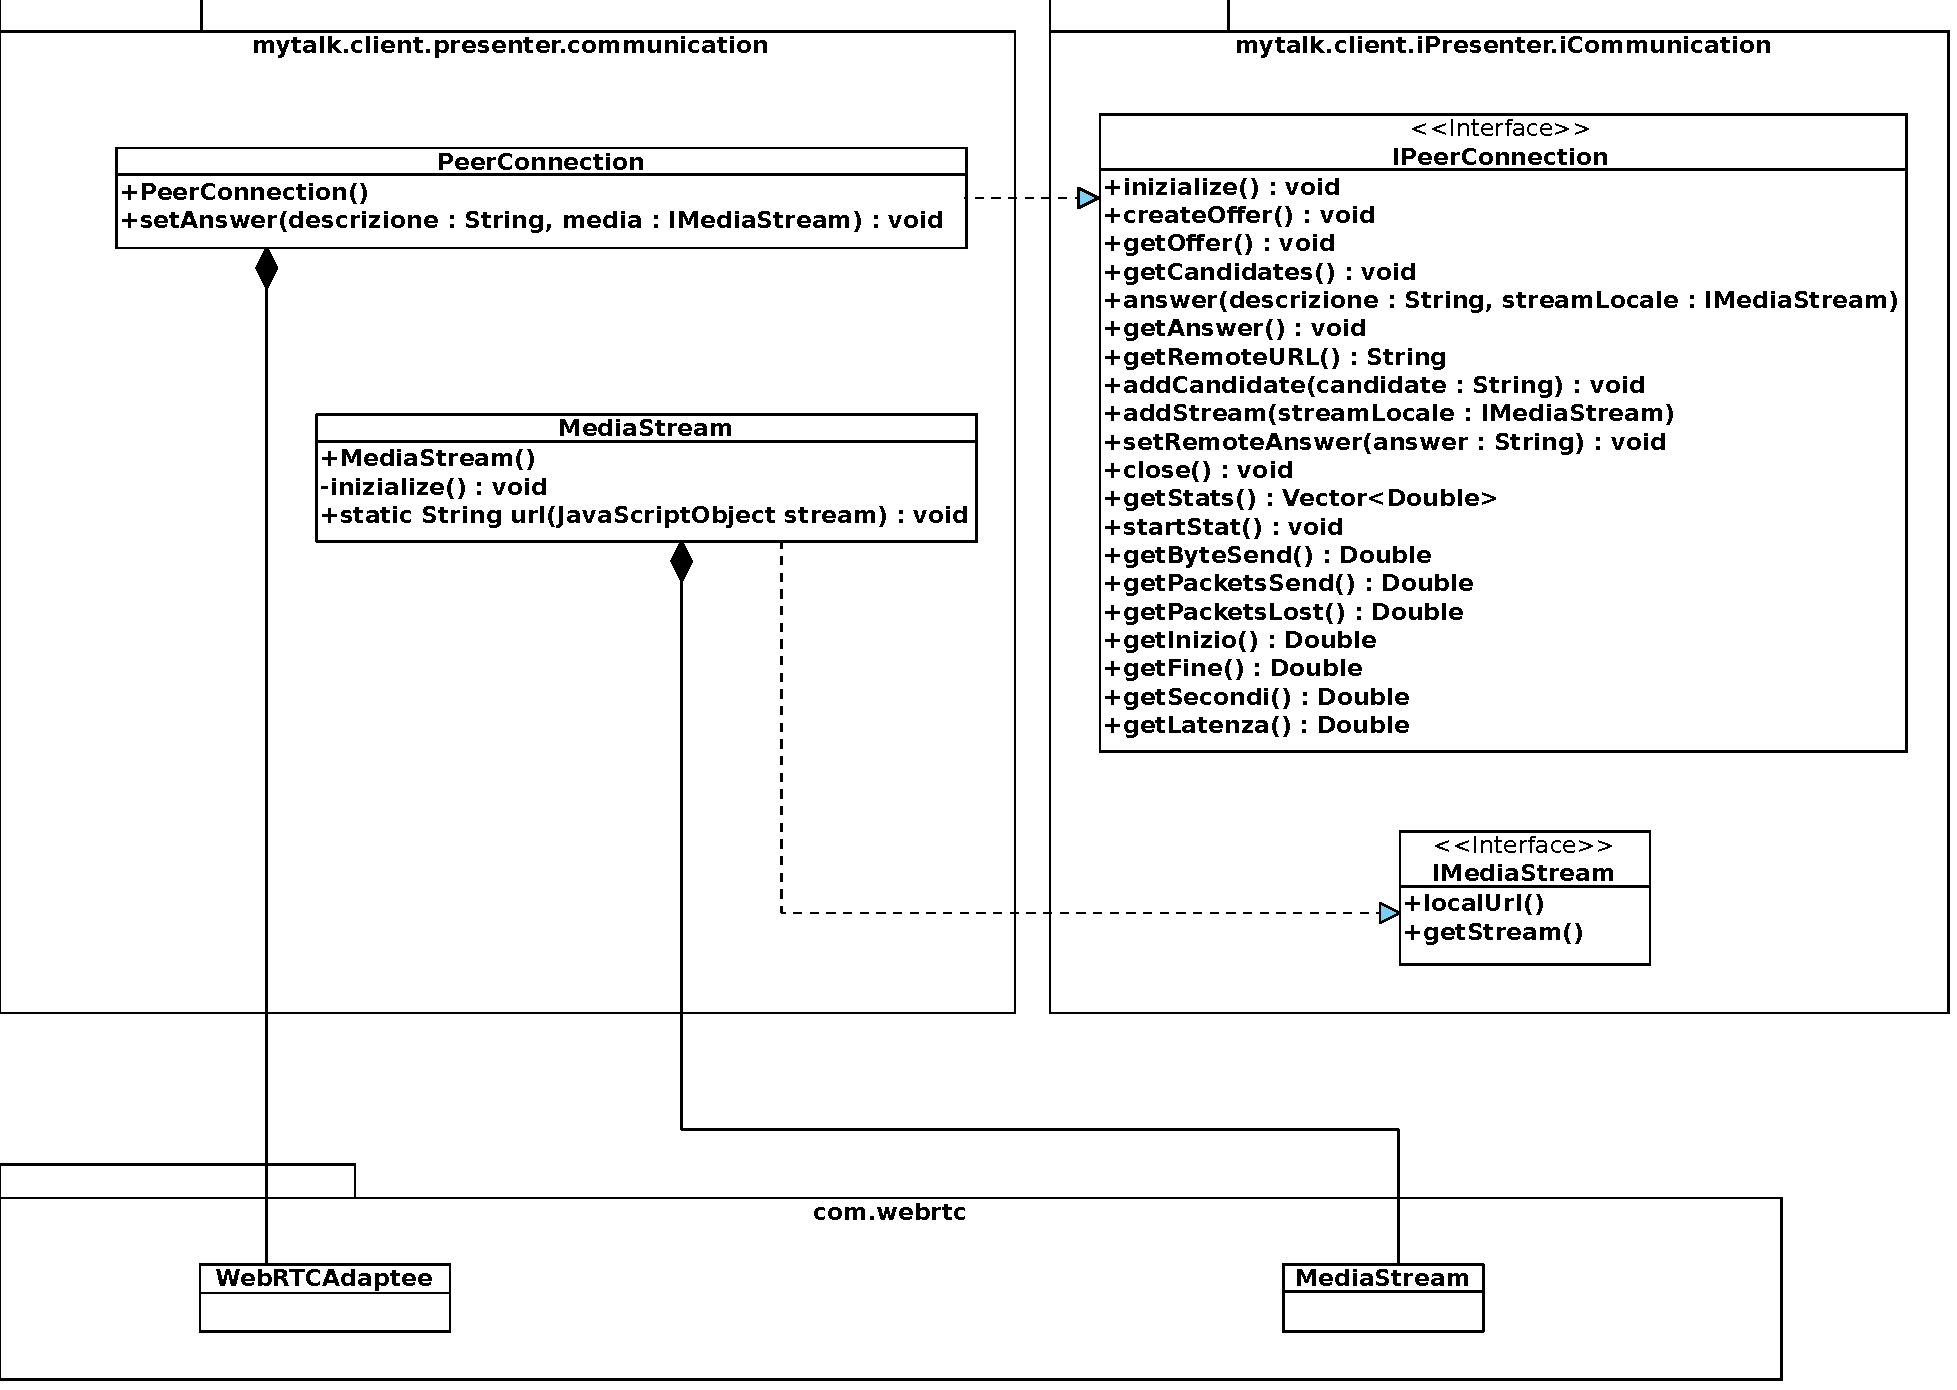
\includegraphics[scale=0.5]{\docsImg classi/presenterCommunication.pdf}
\caption{Diagramma delle classi dei package \nolinkurl{mytalk.client.iPresenter.iUser.iCommunication} e  \nolinkurl{mytalk.client.presenter.user.communication}; dettaglio delle classi \nolinkurl{IPeerConnction}, \nolinkurl{IMediaStream}, \nolinkurl{PeerConnction} e  \nolinkurl{MediaStream}.}
	\end{figure}	
	
					% IMediaStream - inizio
			\paragraph{IMediaStream}\label{par:IMediaStream}{
			\begin{itemize}
				\item[] \textbf{Funzione:}\\
					Le classi che implementano questa interfaccia hanno il compito di ottenere e gestire l'accesso ai dispositivi hardware\g~ che permettono la comunicazione audio e video.\\
			
				\item[] \textbf{Relazioni con altre componenti:}{\\
					L'interfaccia è implementata da:
					\begin{itemize}
				 		\item[]	\path{mytalk.client.presenter.user.communication.MediaStream}.
					\end{itemize} 		
					L'interfaccia è utilizzata da:
					\begin{itemize}
						\item[] \path{mytalk.client.presenter.user.logicUser.CommunicationLogic}.\\
					\end{itemize}					
				}
				
				\item[] \textbf{Metodi:}{\\
					\texttt{+ String localURL();}\\
					Restituisce l'URL\g~ associato ad uno stream\g~ locale, altrimenti una stringa inizializzata a \texttt{null}.\\

					\texttt{+ JavaScriptObject getStream();}\\
					Restituisce l'oggetto JavaScript\g~ che rappresenta lo stream\g~ locale al quale l'utente ha precedentemente consentito l'acquisizione.\\
				}
			\end{itemize}
			}
			% IMediaStream - fine
	
	

			% IPeerConnection - inizio
			\paragraph{IPeerConnection}\label{par:IPeerConnection}{
			\begin{itemize}
			
				\item[] \textbf{Funzione:}\\
				L'interfaccia fornisce le funzioni fondamentali per la gestione della connessione per gli utenti che vogliono comunicare.\\
			
				\item[] \textbf{Relazioni con altre componenti:}\\
					L'interfaccia è implementata da:
					\begin{itemize}
						\item[]	\path{mytalk.client.presenter.user.communication.PeerConnection}.
					\end{itemize} 		
					L'interfaccia è utilizzata da:
					\begin{itemize}
						\item[] \path{mytalk.client.presenter.user.logicUser.CommunicationLogic}.\\
					\end{itemize}
				
				\item[] \textbf{Metodi:}\\
					\texttt{+ void inizialize();}\\
					Inizializza i campi dati della connessione.\\
					
					\texttt{+ void answer(String descrizione, IMediaStream stream);}\\
					Aggiunge uno stream\g~ locale alla connessione e crea una risposta che poi sarà inviata ad un utente. Per risposta si intende una descrizione di sessione di tipo \texttt{Answer}.\\
					
					\texttt{+ String getAnswer();}\\
					Restituisce un oggetto in un formato assegnabile ad una stringa che descrive la sessione locale da inviare come risposta ad un altro ricevuto in precedenza.\\

					\texttt{+ String getCandidates();}\\
					Restituisce una stringa da inviare ad un utente remoto contenente tutti i candidati ICE creati in precedenza.\\

					\texttt{+ String getOffer();}\\
					Restituisce un oggetto in un formato assegnabile ad una stringa che descrive la sessione locale da inviare ad un utente remoto.\\

					\texttt{+ String getRemoteURL();}\\
					Restituisce l'URL\g~ dello stream\g~ remoto eventualmente esistente, altrimenti una stringa vuota.\\

					\texttt{+ void createOffer();}\\
					Crea una offerta che poi sarà inviata ad un utente. Per offerta si intende una descrizione di sessione di tipo \texttt{Offer}.\\

					\texttt{+ void close();}\\
					Chiude la comunicazione eventualmente in atto.\\

					\texttt{+ Vector<Double> getStats();}\\
					Restituisce un vettore di \texttt{Double} che rappresenta le statistiche da visualizzare nella GUI\g~ o da inviare al server\g.\\

					\texttt{+ void receivedComunication(Vector<String> candidate);}\\
					Imposta i candidati ICE\g~ all'interno dell'oggetto che gestisce la connessione.\\

					\texttt{+ void addCandidate(String candidate);}\\
					Imposta il candidato ICE\g~ all'interno dell'oggetto che gestisce la connessione.\\
					
					\texttt{+ void addStream(IMediaStream stream);}\\
					Aggiunge uno stream\g~ locale all'oggetto che gestisce la connessione.\\
					
					\texttt{+ void setRemoteAnswer(String answer);}\\
					Imposta una descrizione remota di tipo \texttt{answer} all'oggetto che gestisce la connessione.\\
					
					\texttt{+ void startStats();}\\
					Invia un segnale all'oggetto che gestisce la connessione che da inizio al campionamento delle statistiche.\\
					
					\texttt{+ Double getByteSend();}\\
					Ritorna il numero di byte inviati dagli stream\g~ audio e video (la somma dei due).\\

					\texttt{+ Double getPacketsSend();}\\
					Ritorna il numero dei pacchetti inviati dagli stream\g~ audio e video.\\

					\texttt{+ Double getPacketsLost();}\\
					Ritorna il numero di pacchetti persi nel corso della comunicazione dagli stream\g~ audio e video.\\

					\texttt{+ Double getInizio();}\\
					Ritorna il numero di millisecondi intercorsi dalla mezzanotte del 01/01/1970 all'inizio della comunicazione.\\

					\texttt{+ Double getFine();}\\
					Ritorna il numero di millisecondi intercorsi dalla mezzanotte del 01/01/1970 alla fine della comunicazione.\\
					
					\texttt{+ Double getSecondi();}\\
					Ritorna il numero di secondi intercorsi dall'inizio della comunicazione alla chiamata del metodo.\\
					
					\texttt{+ Double getLatenza();}\\
					Ritorna la latenza\g~ dello stream\g~ audio al momento della chiamata del metodo.\\
			\end{itemize}
			}
			% IPeerConnection - fine
	}
	
	\subsubsection{Package mytalk.client.presenter.user.communication}{
	
% MediaStream - inizio
			\paragraph{MediaStream}\label{par:MediaStream}{
			\begin{itemize}
				\item[] \textbf{Funzione:}\\
					La classe gestisce i media locali e richiede il permesso di accesso all'hardware\g~ all'utente.\\
			
				\item[] \textbf{Relazioni con altre componenti:}\\
					Implementa l'interfaccia: 
					\begin{itemize}
						\item[] \path{mytalk.client.iPresenter.iUser.iCommunication.IMediaStream}.
					\end{itemize}
					Usa le classi:
					\begin{itemize}
						\item[] \path{API getUserMedia};
					\end{itemize}
					tramite l'interfaccia:
					\begin{itemize}
						\item[]\path{mytalk.client.iPresenter.iUser.iCommunication.IMediaStream}.\\
					\end{itemize}
		
				\item[] \textbf{Attributi:}{\\
					\texttt{- JavaScriptObject localStream}: l'oggetto garantisce l'accesso all'hardware\g~ locale, se l'oggetto è inizializzato allora l'utente ha acconsentito all'accesso all'hardware\g~ locale(videocamera e microfono oppure solo microfono).\\

					\texttt{- String localURL}: la stringa contiene l'URL\g~ associato allo stream\g~ locale al quale l'utente ha garantito l'accesso, se la stringa è uguale a null allora o l'utente ha rifiutato la richiesta dell'applicazione di accedere all'hardware\g~ oppure non ha ancora dato il consenso.\\
				}
			
				\item[] \textbf{Metodi:}{\\
					\texttt{+ void inizialize();}\\ 
					Inizializza lo stream\g~ con un oggetto che rappresenta e consente l'accesso all'hardware\g~ locale. Per far ciò richiama il metodo dell'oggetto \texttt{JavaScript window.GetUserMedia} che richiede all'utente l'accesso all'hardware\g. Se l'utente acconsente alla richiesta d'accesso allora richiama un metodo che memorizza l'oggetto che rappresenta lo stream\g~ e lo converte in un URL\g.\\

					\texttt{+ String localURL();}\\
					Restituisce l'URL\g~ associato ad uno stream\g~ locale, altrimenti una stringa inizializzata a \texttt{null}.\\

					\texttt{+ JavaScriptObject getStream();}\\
					Restituisce l'oggetto JavaScript\g~ che rappresenta lo stream\g~ locale al quale l'utente ha precedentemente consentito l'acquisizione.\\
				}
			\end{itemize}
			}
			% MediaStream - fine


		

			% PeerConnection - inizio
			\paragraph{PeerConnection}\label{par:PeerConnection}{
			\begin{itemize}
				\item[] \textbf{Funzione:}\\
					La classe permette di gestire i dati delle \texttt{API WebRTC}\g~ e di stabilire connessioni VoIP\g~ peer-to-peer\g.
			
				\item[] \textbf{Relazioni con altre componenti:}\\
					Implementa l'interfaccia: 
					\begin{itemize}
						\item[] \path{mytalk.client.iPresenter.iUser.iCommunication.IPeerConnection}.
					\end{itemize}
					Usa le classi:
					\begin{itemize}
						\item[] \texttt{WebRTCAdaptee}.\\
					\end{itemize}
				
				\item[] \textbf{Attributi:}
					\texttt{- JavaScriptObject WebRTC:} permette di aprire, gestire e chiudere una comunicazione peer-to-peer\g.\\
			
				\item[] \textbf{Metodi:}{\\
					\texttt{+ void inizialize();}\\
					Richiama il metodo \texttt{inizialize()} della classe \texttt{WebRTCAdaptee}. In questo modo l'oggetto che gestisce la connessione viene inizializzato e ne vengono registrati gli eventi utilizzati dall'applicazione.\\
					
					\texttt{+ void addStream(IMediaStream stream);}\\
					Aggiunge uno stream\g~ locale alla connessione, richiama il metodo \texttt{addstream} della classe \texttt{WebRTCAdaptee} per effettuare l'aggiunta dello stream\g, in questo modo lo stream può essere condiviso con l'utente con cui si comunica.\\
					
					\texttt{+ String getRemoteURL();}\\
					Restituisce l'URL\g~ dello stream\g~ remoto richiamando il metodo della classe \texttt{WebRTCAdaptee} \texttt{getRemoteUrl()}, in questo modo lo stream è visualizzabile all'interno di una pagina html5.\\
					
					\texttt{+ void createOffer();}\\
					Richiama il metodo della classe \texttt{WebRTCAdaptee offer()}. In questo modo viene creata una descrizione della sessione locale da inviare ad un altro utente di tipo \texttt{offer}, la descrizione di sessione contiene informazioni come gli stream condivisi e il protocollo utilizzato per creare il canale di comunicazione VoIP.\\
					
					\texttt{+ void answer(String remoteOffer, MediaStream streamLocale);}\\
					Richiama il metodo della classe \texttt{WebRTCAdaptee answer(String remoteOffer, MediaStream streamLocale)} passandogli come parametri la descrizione remota di tipo \texttt{offer} e l'oggetto che rappresenta lo stream\g~ locale. Successivamente vengono impostati lo stream\g~ locale, la descrizione remota e la descrizione locale appena creata, la descrizione di sessione contiene informazioni come gli stream\g~ condivisi e il protocollo utilizzato per creare il canale di comunicazione VoIP.\\

					\texttt{+ void close();}\\
					Chiude la comunicazione eventualmente in atto, richiamando il metodo della classe \texttt{WebRTCAdaptee close()}, reinizializzando i campi dati a null.\\
					
					\texttt{+ String getAnswer();}\\
					Restituisce un oggetto in un formato JSON\g~ che descrive la sessione locale da inviare come risposta ad un altro ricevuto in precedenza.\\
					
					\texttt{+ String getOffer();}\\
					Restituisce un oggetto in un formato JSON\g~ che descrive la sessione locale da inviare ad un utente remoto.\\

					\texttt{+ String getCandidates();}\\
					Restituisce una stringa da inviare ad un utente remoto contenente tutti i candidati ICE creati in precedenza.\\

					\texttt{+ void receivedComunication(Vector<String> candidate);}\\
					Imposta i candidati ICE (oggetti WebRTC che contengono informazioni su un peer, informazioni come indirizzo IP, porta del sistema utilizzabile per la comunicazione e protocollo di comunicazione) all'interno dell'oggetto che gestisce la connessione. Per far ciò richiama per ogni elemento dell'array passato come parametro il metodo \texttt{addCandidate(String ice)} dell'oggetto della classe \texttt{WebRTCAdaptee}.\\

					\texttt{- void setAnswer(String descrizione,IMediaStream media);}\\
					Imposta un oggetto \texttt{RTCSessionDescrption} di tipo \texttt{answer} all'interno dell'oggetto di tipo \texttt{webkitRTCPeerConnection}, interno alla classe \texttt{WebRTCAdaptee}, in questo modo viene impostata la descrizione di sessione inviata dall'altro utente, mancano tuttavia gli ICE candidate per iniziare la connessione, tali candidati verranno inviati successivamente.

					\texttt{+ void setRemoteAnswer(String answer);}\\
					Imposta una descrizione remota di tipo 'answer' all'oggetto che gestisce la connessione.\\

					\texttt{+ Vector<Double> getStats();}\\
					Restituisce un vettore di \texttt{Double} che rappresentano le statistiche da visualizzare nella GUI\g~ o da inviare al server\g. Per estrapolare le statistiche si serve del metodo della classe \texttt{RTCPeerConnection getStats()} dal quale riceve un array associativo che contiene le statistiche.\\

					\texttt{+ void addCandidate(String candidate);}
					Il metodo riceve in input un oggetto di tipo \texttt{RTCIceCandidate} codificato in formato JSON\g~ e invoca il metodo della classe \texttt{WebRTCAdaptee addCandidate()} con lo scopo di aggiungere il candidato ICE all'oggetto che rappresenta la connessione.\\
					
					\texttt{+ void startStats();}\\
					Invia un segnale all'oggetto che gestisce la connessione che dà inizio al campionamento delle statistiche. Il segnale è rappresentato dalla chiamata del metodo \texttt{startStat()} dell'oggetto \texttt{WebRTCAdaptee}.\\
					
					\texttt{+ Double getByteSend();}\\
					Invoca \texttt{WebRTCAdaptee getByteSend()} dal quale riceve il numero di byte inviati dagli stream\g~ audio e video(la somma dei due).\\

					\texttt{+ Double getPacketsSend();}\\
					Invoca \texttt{WebRTCAdaptee getPacketsSend()} dal quale riceve il numero dei pacchetti inviati dagli stream\g~ audio e video.\\

					\texttt{+ Double getPacketsLost();}\\
					Invoca \texttt{WebRTCAdaptee getPacketsSend()} dal quale riceve il numero di pacchetti persi nel corso della comunicazione dagli stream\g~ audio e video.\\

					\texttt{+ Double getInizio();}\\
					Invoca \texttt{WebRTCAdaptee getDataInizio()} dal quale riceve il numero di millisecondi intercorsi dalla mezzanotte del 01/01/1970 all'inizio della comunicazione.\\

					\texttt{+ Double getFine();}\\
					Invoca \texttt{WebRTCAdaptee getDataFine()} dal quale riceve il numero di millisecondi intercorsi dalla mezzanotte del 01/01/1970 alla fine della comunicazione.\\
					
					\texttt{+ Double getSecondi();}\\
					Invoca \texttt{WebRTCAdaptee getSeconds()} dal quale riceve il numero di secondi intercorsi dall'inizio della comunicazione alla chiamata del metodo.\\
					
					\texttt{+ Double getLatenza();}\\
					Invoca \texttt{WebRTCAdaptee getJitter()} dal quale riceve la latenza\g~ dello stream\g~ audio al momento della chiamata del metodo.\\
				}
			\end{itemize}
			}
			% PeerConnection - fine
	}	
	
	
	
	%\newpage

		% WebRTCAdaptee - inizio
		\paragraph{WebRTCAdaptee}\label{par:WebRTCAdaptee}{
		
	\begin{figure}[h!tbp]
		\centering
		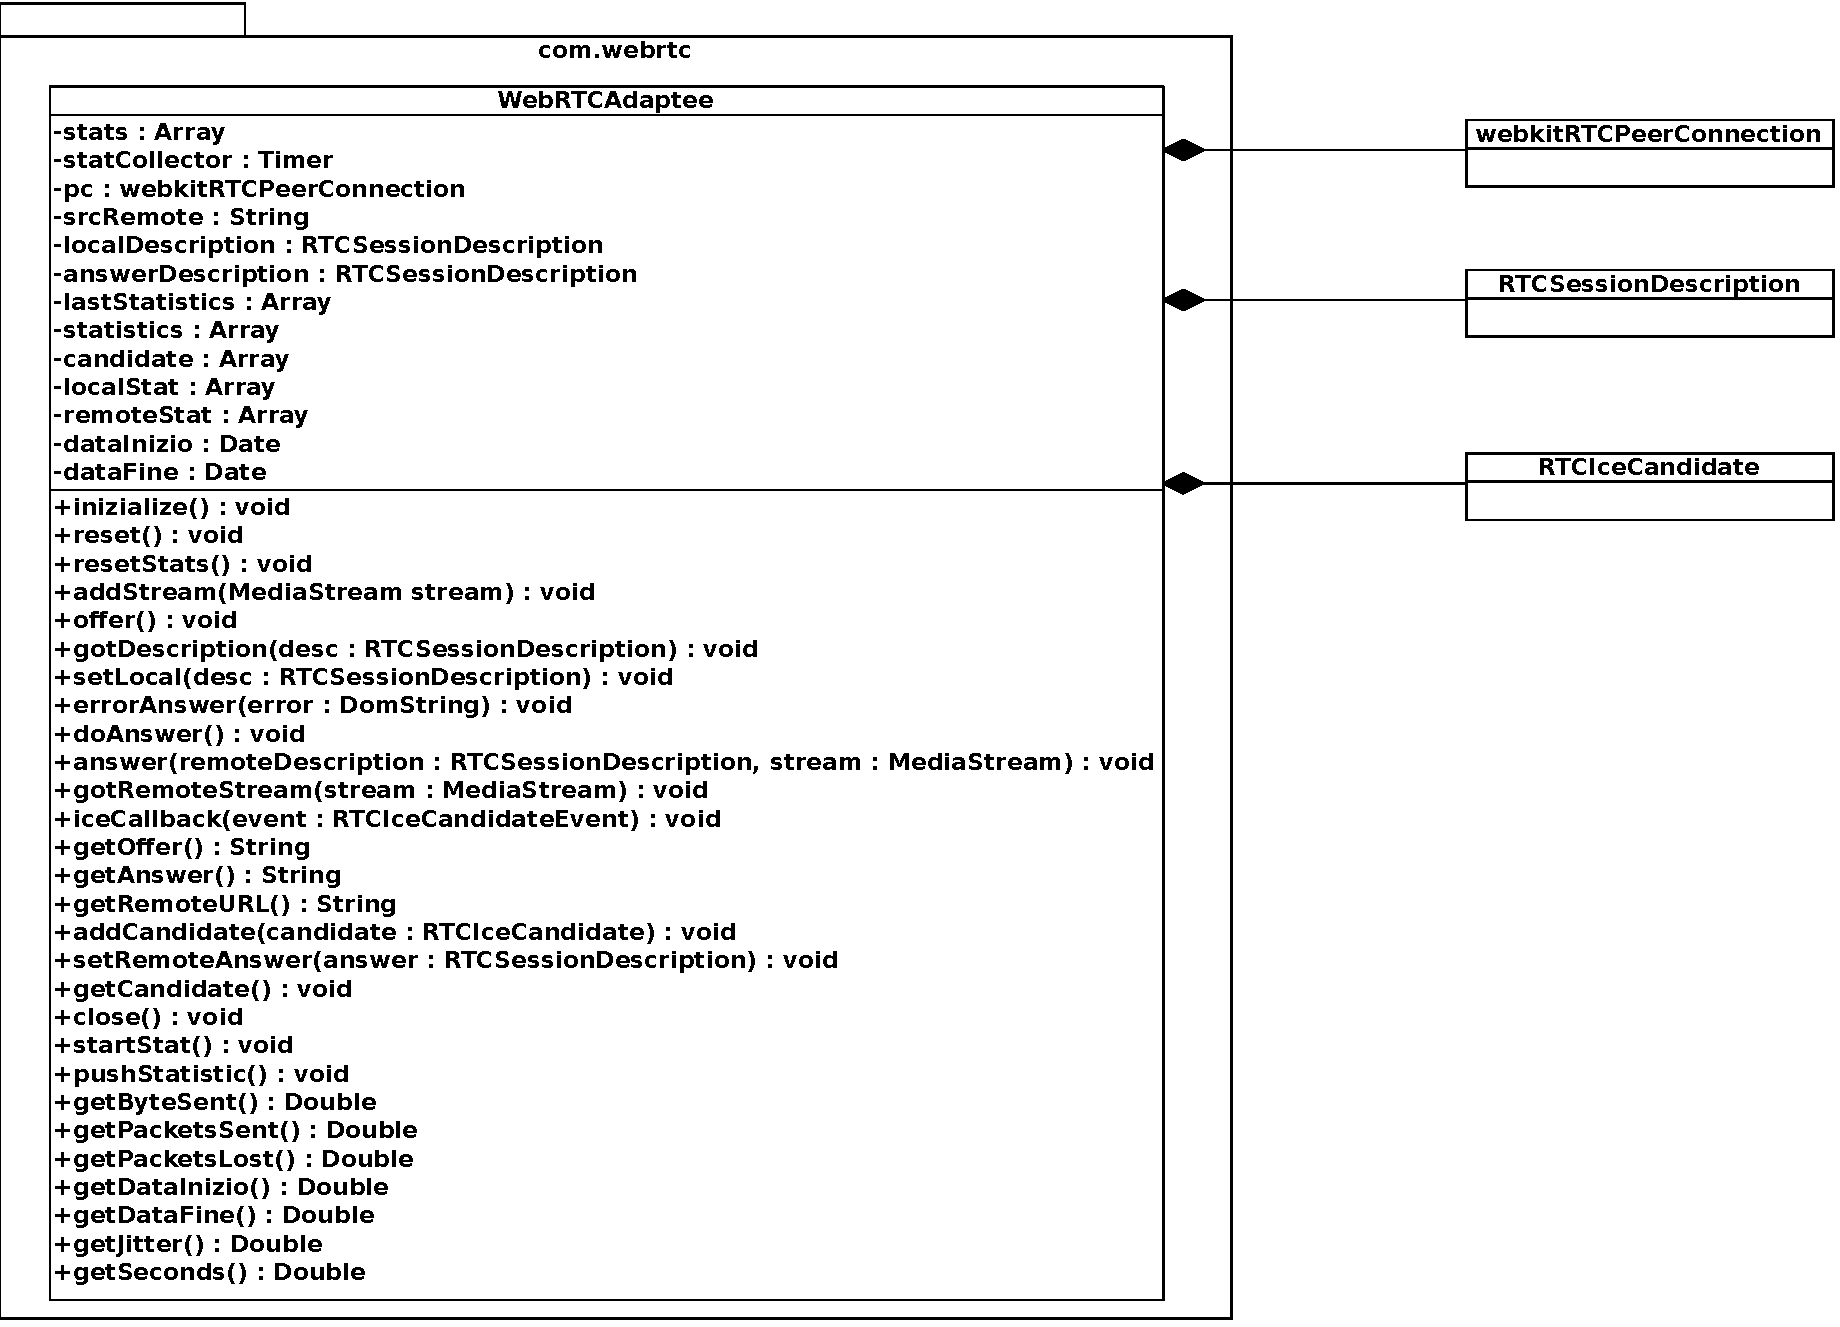
\includegraphics[scale=0.5]{\docsImg classi/WebRTC.pdf}
	\caption{Diagramma delle classi del package \nolinkurl{com.webrtc}; dettaglio della classe \nolinkurl{WebRTCAdaptee}.}
	\label{fig:webRTCadaptee}
	\end{figure}
		
			\begin{itemize}
				
				\item[] \textbf{Funzione:}{\\
					La classe permette di gestire i dati delle \texttt{API WebRTC\g~} e di stabilire connessioni VoIP\g~ peer-to-peer\g.\\
				}
			
				\item[] \textbf{Relazioni con altre componenti:}{\\
					Usa le classi:
					\begin{itemize}
						\item[] \texttt{API WebRTC};
						\item[] \texttt{JavaScript.Date};
						\item[] \texttt{JavaScript.Array}.\\
					\end{itemize}
				}
				
				\item[] \textbf{Attributi:}{\\
				\texttt{- Array stats}: riferimento all'oggetto che raccoglie le statistiche.\\
					
					\texttt{- Array statsCollector}: riferimento all'oggetto che contiene lo storico di tutte le statistiche campionate dalla creazione della connessione.\\
					
					\texttt{- webkitRTCPeerConnection pc}: riferimento, possibilmente nullo, all'oggetto \texttt{RTCPeerConnection} che gestisce la connessione.\\
					
					\texttt{- String srcRemote}: URL\g~ dello stream\g~ remoto, in modo da permetterne la visualizzazione tramite l'interfaccia grafica. Il riferimento è nullo se l'URL\g~ remoto non è ancora stato estratto dalla descrizione remota.\\
					
					\texttt{- String localDescription}: il campo contiene, se diverso da \texttt{null}, la descrizione della sessione locale codificata secondo il formato JSON\g.\\
		
					\texttt{- String answerDescription}: il campo contiene, se diverso da \texttt{null}, la descrizione della sessione locale di tipo \texttt{answer} codificata secondo in formato JSON\g.\\
		
					\texttt{- Array lastStatistics}: il campo contiene le ultime statistiche campionate.\\
		
					\texttt{- Array candidate}: l'array contiene, se non vuoto, i candidati ICE registrati all'atto della creazione della sezione locale.\\
					
					\texttt{- int DataInizio}: millisecondi intercorsi dalla mezzanotte del 01/01/1970 all'inizio della chiamata.\\
					
					\texttt{- int DataFine}: millisecondi intercorsi dalla mezzanotte del 01/01/1970 alla fine della chiamata.\\
				}
			
				\item[] \textbf{Metodi:}{\\
					\texttt{+ void inizialization();}\\
					Inizializza il campo dati \texttt{pc} e ne registra gli eventi.\\
					
					\texttt{+ void addStream(Stream stream);}\\
					Aggiunge uno stream\g~ locale alla connessione.\\
					
					\texttt{+ void offer();}\\
					Crea un oggetto \texttt{RTCSessionDescription} di tipo \texttt{offer}. Se la creazione ha successo viene chiamato il metodo di callback \texttt{gotDescription(RTCSessionDescription description)}.\\		
							
					\texttt{+ void gotDescription(RTCSessionDescription description);}\\
					Salva il parametro \texttt{description} come una stringa JSON\g~ nel campo dati \texttt{localDescription} e imposta l'oggetto come descrizione della sessione locale tramite la chiamata al metodo \texttt{SetLocalDescription} della classe \texttt{webkitRTCPeerConnection}.\\
					
					\texttt{+ String getRemoteURL();}\\
					Restituisce l'URL\g~ dello stream\g~ remoto se esiste, \texttt{null} altrimenti.\\
					
					\texttt{+ void iceCallback(event e);}\\
					Metodo di callback che viene invocato quando viene creato un oggetto \texttt{RTCIceCandidate} in seguito alla creazione di un oggetto \texttt{RTCSessionDescription}. Il metodo converte l'oggetto \texttt{RTCIceCandidate} in una stringa JSON\g~ e lo salva nell'array \texttt{candidate}.\\
					
					\texttt{+ void answer(RTCSessioneDescription descrizione, Stream stream);}\\
					Reinizializza il campo dati \texttt{pc}, aggiunge all'oggetto \texttt{pc} lo stream\g~ locale passato come parametro di nome \texttt{stream}. Imposta come descrizione di sessione remota l'oggetto \texttt{descrizione} passato come parametro e crea una descrizione di sessione tramite la chiamata al metodo \texttt{doAnswer()}.
					
					\texttt{+ void doAnswer();}\\
					Richiama il metodo \texttt{createAnswer()} delle WebRTC\g~ sull'oggetto \texttt{pc} al fine di creare una descrizione di sessione di tipo \texttt{answer}. Se la creazione dell'oggetto ha successo viene richiamato il metodo di callback \texttt{setLocal(RTCSessionDescription description)}, altrimenti viene richiamato il metodo \texttt{errorAnswer()}.\\
					
					\texttt{+ void setLocal(RTCSessionDescription descrizione);}\\
					Metodo di callback che viene invocato se la creazione di un oggetto \texttt{RTCSessionDescription} di tipo \texttt{answer} ha avuto successo. Il metodo salva l'oggetto in formato JSON\g~ nel campo dati \texttt{answerDescription} e imposta l'oggetto come descrizione della sessione locale tramite la chiamata al metodo \texttt{SetLocalDescription} della classe \texttt{webkitRTCPeerConnection}.\\

					\texttt{+ void errorAnswer(string answer);}\\
					Il metodo viene invocato se vi è stato un errore nella creazione dell'oggetto \texttt{RTCSessionDescription} di tipo \texttt{answer}.\\
					
					\texttt{+ void close();}\\
					Chiude la comunicazione eventualmente in atto richiamando il metodo della classe \texttt{RTCPeerConnection close()} sull'oggetto \texttt{pc}. Ferma il campionamento delle statistiche e dopo 2 secondi dalla chiusura reinizializza tutti i campi dati per prepararli ad una nuova eventuale comunicazione.\\

					\texttt{+ void addCandidate(String candidate);}
					Aggiunge un candidato ICE alla connessione chiamando il metodo della classe \texttt{webkitRTCPeerConnection addIceCandidate(RTCIceCandidate iceCandidate)}.\\
					
					\texttt{+ void startStats();}\\
					Imposta un intervallo che campiona le statistiche una volta ogni secondo. Per ottenere le statistiche si serve della funzione delle WebRTC\g~ \texttt{getStats()} che viene invocata sull'oggetto \texttt{pc} di tipo \texttt{webkitRTCPeerConnection}.\\
					
					\texttt{+ void setRemoteAnswer(String answer);}\\
					Il metodo riceve in input un oggetto \texttt{RTCSessioneDescription} di tipo \texttt{answer} e lo imposta come descrizione remota tramite il metodo dell'oggetto \texttt{webkitRTCPeerConnection setRemoteDescription(RTCSessionDescription description)}.\\
					
					\texttt{+ Double getByteSend();}\\
					Ritorna il numero di byte inviati dagli stream\g~ audio e video(la somma dei due).\\

					\texttt{+ Double getPacketsSend();}\\
					Ritorna il numero dei pacchetti inviati dagli stream\g~ audio e video.\\

					\texttt{+ Double getPacketsLost();}\\
					Ritorna il numero di pacchetti persi nel corso della comunicazione dagli stream\g~ audio e video.\\

					\texttt{+ Double getDataInizio();}\\
					Ritorna il numero di millisecondi intercorsi dalla mezzanotte del 01/01/1970 all'inizio della comunicazione.\\

					\texttt{+ Double geDatatFine();}\\
					Ritorna il numero di millisecondi intercorsi dalla mezzanotte del 01/01/1970 alla fine della comunicazione.\\
					
					\texttt{+ Double getSeconds();}\\
					Ritorna il numero di secondi intercorsi dall'inizio della comunicazione alla chiamata del metodo.\\
					
					\texttt{+ Double getJitter();}\\
					Ritorna la latenza\g~ dello stream\g~ audio al momento della chiamata del metodo.\\
					
					\texttt{+ void reset();}\\
					Assegna il valore \texttt{null} a tutti i campi dati della classe per iniziare una nuova comunicazione.\\
					
					\texttt{+ void resetStats();}\\
					Cancella tutti i campionamenti delle statistiche avvenuti nell'ultima chiamata.\\
					
					\texttt{+ void getOffer();}\\
					Restituisce un oggetto di classe \texttt{RTCSessionDescription} di tipo \texttt{Offer} in formato JSON\g~ se è stato creato in precedenza \texttt{null} altrimenti.\\
					
					\texttt{+ void getAnswer();}\\
					Restituisce un oggetto di classe \texttt{RTCSessionDescription} di tipo \texttt{Answer} in formato JSON\g~ se è stato creato in precedenza \texttt{null} altrimenti.\\
					
					\texttt{+ void getCandidate();}\\
					Restituisce gli oggetti di classe \texttt{RTCICeCandidate} in formato JSON\g~ creati in precedenza.\\
				}
			\end{itemize}
			}
		% WebRTCAdaptee - fine
	}
	
	
	
	
\newpage
	\subsubsection{Package mytalk.client.iPresenter.iAdministrator.iLogicAdmin}{
			
		\begin{figure}[h!tbp]
		\centering
		\label{fig:adminLogicAdmin}
		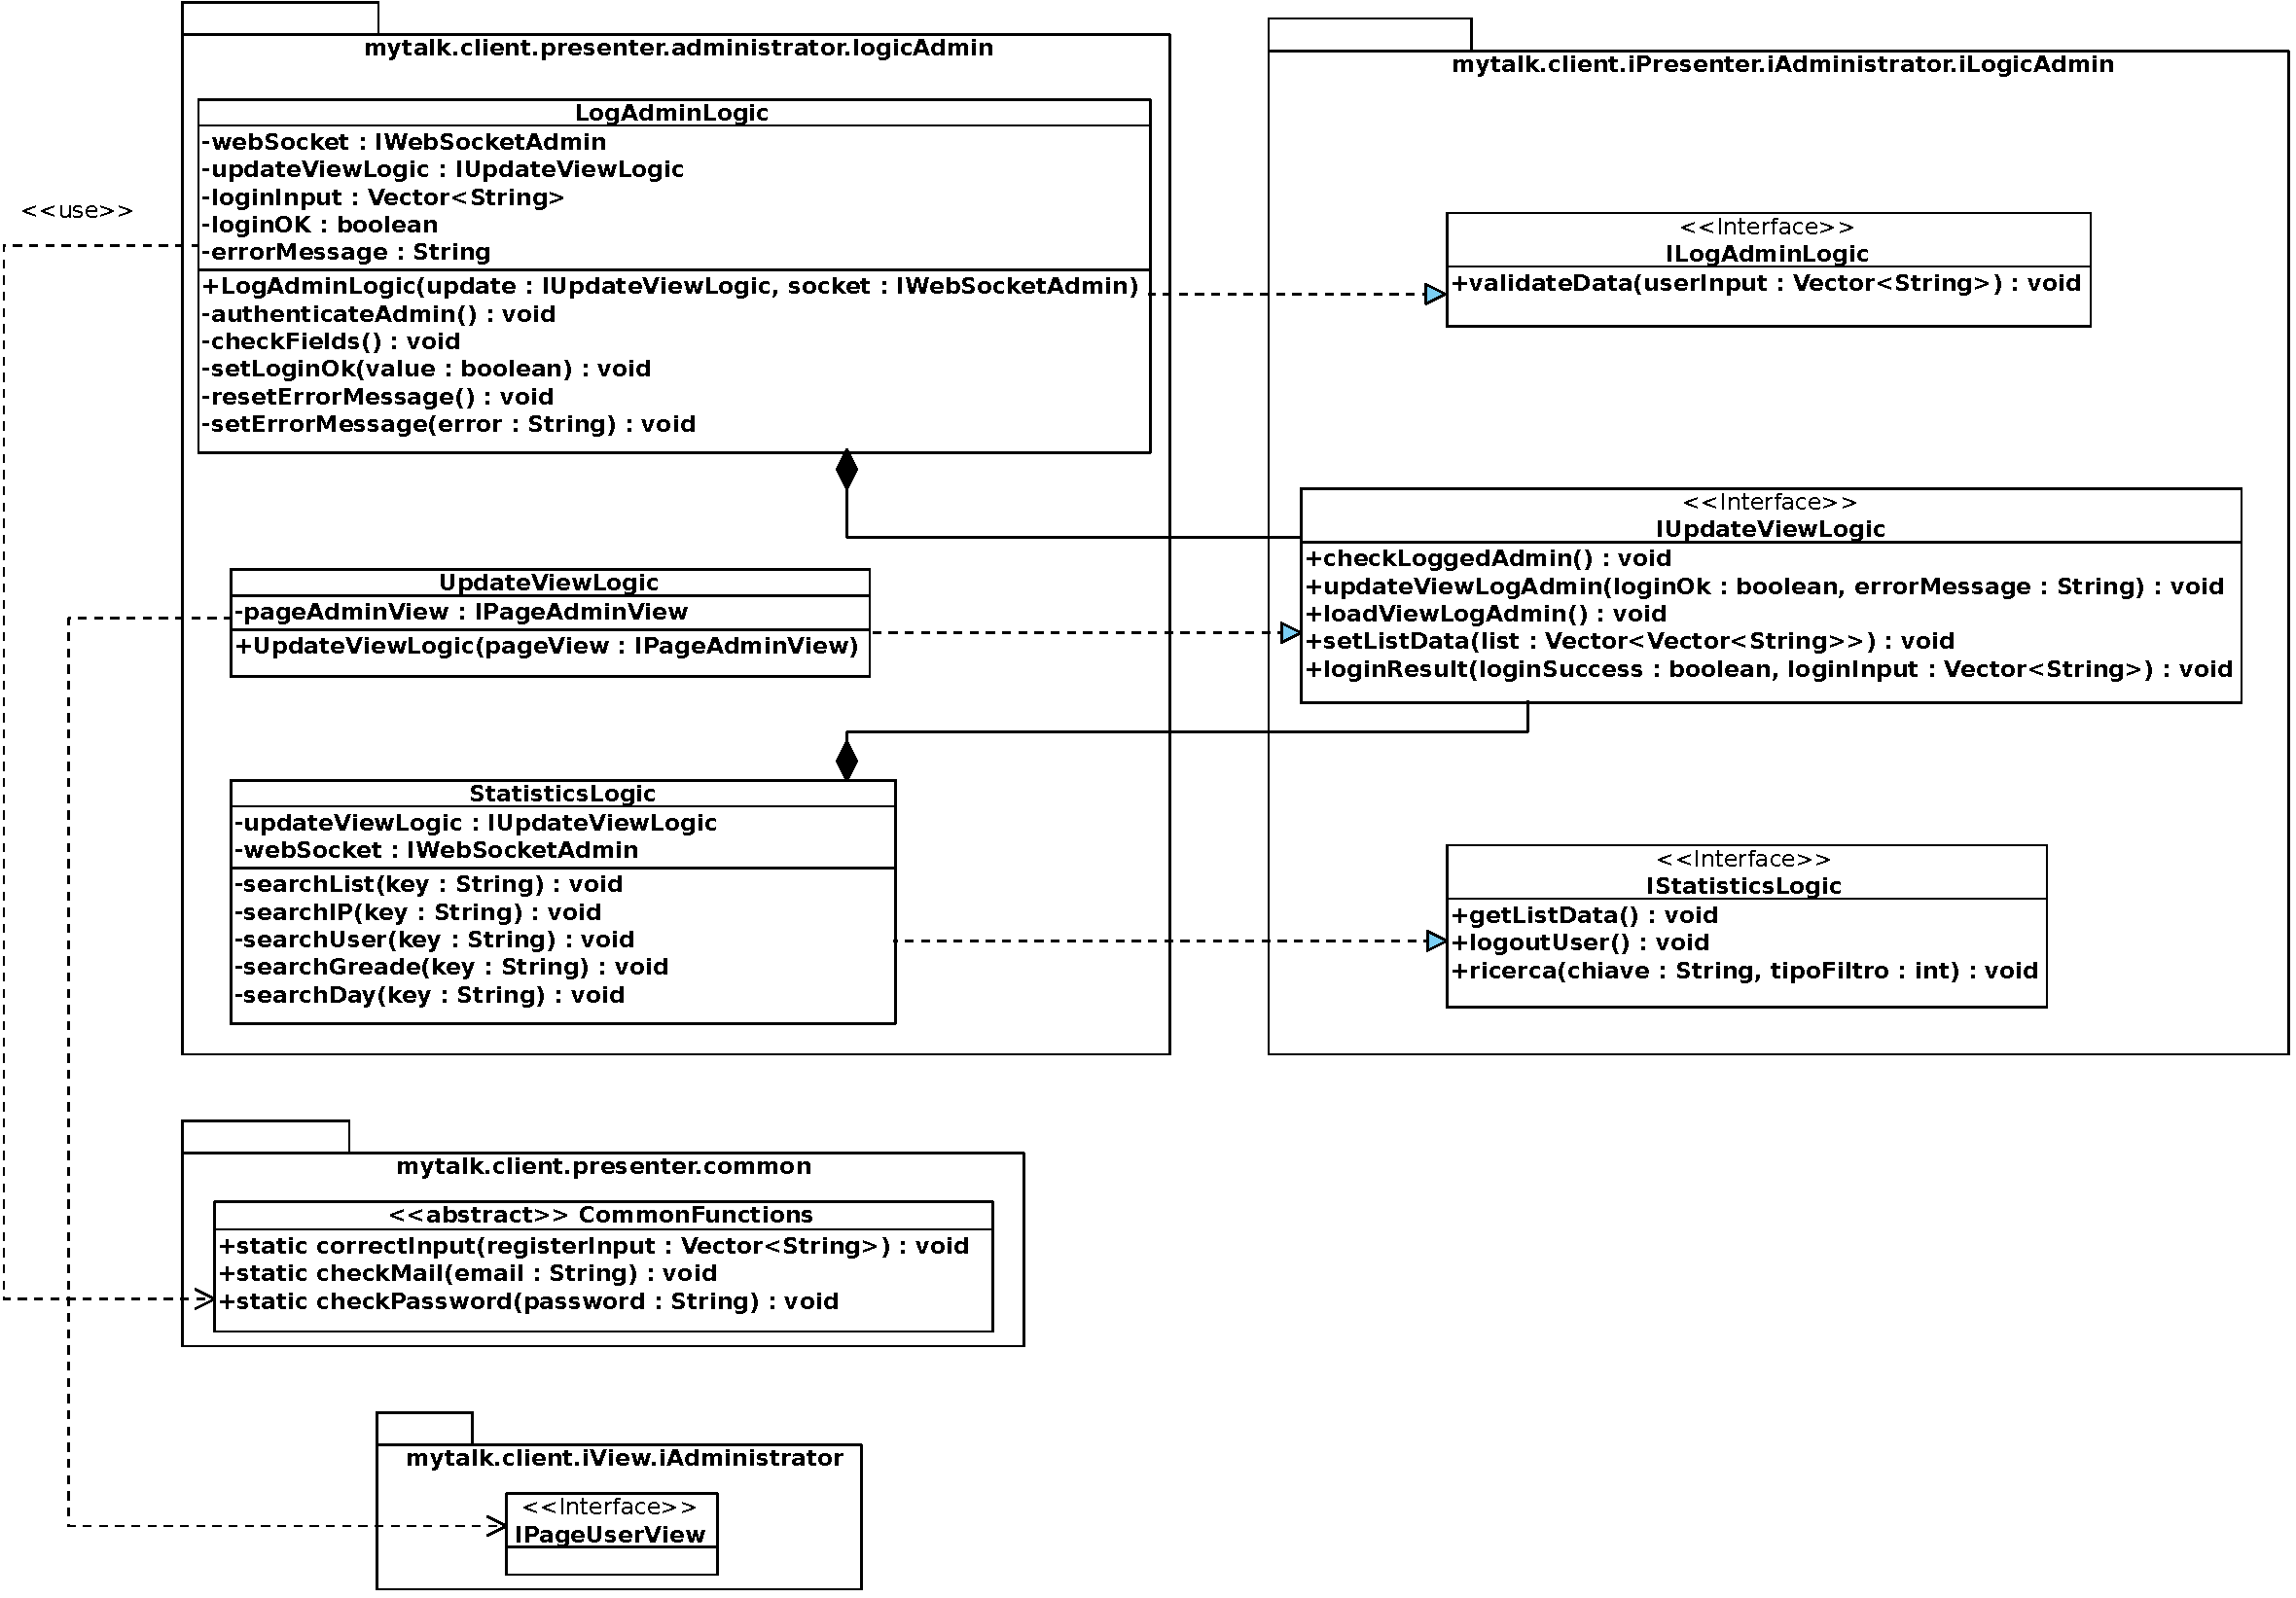
\includegraphics[scale=0.45]{\docsImg classi/presenterClientAdmin.pdf}
\caption{Diagramma delle classi dei package \nolinkurl{mytalk.client.iPresenter.iAdministrator.iLogicAdmin} e  \nolinkurl{mytalk.client.presenter.administrator.logicAdmin}; dettaglio delle classi \nolinkurl{ILogAdminLogic}, \nolinkurl{IUpdateViewLogic}, \nolinkurl{IStatisticsLogic}, \nolinkurl{LogAdminLogic}, \nolinkurl{UpdateViewLogic} e \nolinkurl{StatisticsLogic}.}
	\end{figure}	

		% ILogAdminLogic - inizio
		\paragraph{ILogAdminLogic}\label{par:ILogAdminLogic}{
			\begin{itemize}
				\item[] \textbf{Funzione:}\\
				Interfaccia che offre operazioni logiche alle classi della View.\\
			
				\item[] \textbf{Relazioni con altre componenti:}{\\
					L'interfaccia è implementata da:
					\begin{itemize}
						\item[] \path{mytalk.client.presenter.administrator.logicAdmin.LogAdminLogic}.
					\end{itemize} 
					L'interfaccia è utilizzata da:
					\begin{itemize}
						\item[] \path{mytalk.client.view.administrator.LogAdminView}.\\
					\end{itemize}
				}
			
				\item[] \textbf{Metodi:}{ \\
					\texttt{+ void validateData(Vector<String> userInput);}\\
					Controlla che il vettore \texttt{userInput} contenga valori conformi ai formati e richiede di controllare che tali valori siano anche presenti nel server\g.\\
				}
			\end{itemize}
			}
		% ILogAdminLogic - fine
		
		
		

		% IStatisticLogic - inizio
		\paragraph{IStatisticLogic}\label{par:IStatisticLogic}{
			\begin{itemize}

				\item[] \textbf{Funzione:}\\
					L'interfaccia fornisce i metodi tramite i quali l'utente amministratore può richiedere le statistiche al server\g.\\
			
				\item[] \textbf{Relazioni con altre componenti:}{\\
					L'interfaccia è implementata da:
					\begin{itemize}
						\item[] \path{mytalk.client.presenter.administrator.logicAdmin.StatisticLogic}.
					\end{itemize}
					L'interfaccia è utilizzata da:
					\begin{itemize}
						\item[] \path{mytalk.client.view.user.StatisticView};\\
					\end{itemize}
				}
			
				\item[] \textbf{Metodi:}{ \\
				 	\texttt{+ void getListData();}\\
					Richiede al server\g~ l'intera lista delle statistiche presenti nel database.\\
					
					\texttt{+ void logoutUser();}\\
					Richiede al server\g~ l'uscita dal servizio da parte dell'utente amministratore attualmente autenticato.\\
					
					\texttt{+ void ricerca(String chiave, int tipoFiltro);}\\
					Richiede al server\g~ un sottoinsieme delle statistiche, filtrate per un qualche valore.\\
					
					\texttt{+ void setUserList();}\\
					Richiede al server la lista di utenti registrati al servizio.\\
				}
			\end{itemize}
			}
		% IStatisticLogic - fine


		

		
		% IUpdateViewLogic - inizio
		\paragraph{IUpdateViewLogic}\label{par:IUpdateViewLogic}{
			\begin{itemize}
				\item[]  \textbf{Funzione:} \\
				Interfaccia che offre operazioni alle classi che devono interagire con la View.\\
				
				\item[]  \textbf{Relazioni con altre componenti:} \\
				L'interfaccia è implementata da:
				\begin{itemize}
					\item[-] \path{mytalk.client.view.administrator.UpdateViewLogic}.
				\end{itemize}
				L’interfaccia è utilizzata da:
				\begin{itemize}
					\item[-] \path{mytalk.client.view.administrator.PageAdminView}.\\
				\end{itemize}
				
				\item[]  \textbf{Metodi:}\\
					\texttt{+ void checkLoggedAdmin();}\\
					Controlla l’esistenza di cookies\g~ di sessione.\\
					
					\texttt{+ void updateViewLogAdmin(boolean loginOk, String errorMessage);}\\
					Invia alla View il risultato dell’operazione di autenticazione.\\
					
					\texttt{+ void loadViewLogAdmin();}\\
					Richiede alla grafica il caricamento della GUI\g~ di autenticazione dell’amministratore.\\
					
					\texttt{+ void setListData(Vector<Vector<String>> list);}\\
					Invia i dati delle statistiche alla View.\\
					
					\texttt{+ void loginResult(boolean loginSuccess, Vector<String> loginInput);}\\
					A seconda del valore di \texttt{loginSuccess} crea i cookie\g~ o ritorna un’errore di autenticazione:
					\begin{itemize}
						\item[-] se è \texttt{true}: crea il cookie\g~ e richiede l’aggiornamento della View;
						\item[-] se è \texttt{false}: imposta l’errore da ritornare e richiede l’aggiornamento della View.\\
					\end{itemize}
					
					\texttt{+ void errorViewFilter(String string);}\\
					Richiede la visualizzazione dell’errore contenuto in \texttt{String}.\\
					
					\texttt{+ void setUserList(Vector<String> listaUtenti);}\\
					Invia alla View la lista degli utenti registrati.\\
					
					\texttt{+ void removeCookies();}\\
					Rimuove i cookie\g.\\
					
					\texttt{+ void setUsernameLabel();}\\
					Invia alla View il nome utente salvato nel cookie\g.\\
			\end{itemize}
			}
		% IUpdateViewLogic - fine
		
	}
	
	\subsubsection{Package mytalk.client.presenter.administrator.logicAdmin}{


% LogAdminLogic - inizio
		\paragraph{LogAdminLogic}\label{par:LogAdminLogic}{
				\begin{itemize}
					\item[] \textbf{Funzione:}{\\
					La classe ha il compito di effettuare controlli di logica e di inviare i risultati ad altri metodi per il controllo o inviare i dati alla View per aggiornarla.\\
					}
				
					\item[] \textbf{Relazioni con altre componenti:}{\\
					Implementa l'interfaccia:
					\begin{itemize}
						\item[]	\path{mytalk.client.iPresenter.iAdministrator.iLogicAdmin.ILogAdminLogic}.
					\end{itemize} 		
					Usa le classi:
					\begin{itemize}
						\item[] \path{mytalk.client.presenter.administrator.logicAdmin.UpdateViewLogic};
						\item[] \path{mytalk.client.presenter.administrator.serverComUser.WebSocketAdmin};
					\end{itemize}
					tramite le interfacce:
					\begin{itemize}
						\item[] \path{mytalk.client.iPresenter.iAdministrator.iLogicAdmin.IUpdateViewLogic};
						\item[] \path{mytalk.client.iPresenter.iAdministrator.iServerComUser.IWebSocketAdmin}.\\
					\end{itemize}
					}

					\item[] \textbf{Attributi:}{\\
						\texttt{- IWebSocketAdmin webSocket:} riferimento alla classe \texttt{WebSocketAdmin}.
							Permette di richiamare i metodi per i controlli dei dati da parte del server.\\

						\texttt{- IUpdateViewLogic updateViewLogic:} riferimento alla classe UpdateViewLogic.
						Permette di richiamare metodi per l'aggiornamento della GUI\g~.\\

						\texttt{- Vector<String> loginInput:} contenitore per i dati inseriti dall'utente in fase di autenticazione.\\

						\texttt{- boolean loginOk:} valore booleano\g~ che indica se il controllo del formato dei dati è andato a buon fine.\\

						\texttt{- String errorMessage:} Stringa contenente il messaggio di errore complessivo.\\
					}
					
					\item[] \textbf{Metodi:}{ \\
					\texttt{+LogAdminLogic(IUpdateViewLogic updateViewLogic, IWebSocketAdmin webSocket);}\\
					Costruttore: inizializza gli oggetti \texttt{updateViewLogic} e \texttt{webSocket}. Imposta a \texttt{true} il valore di \texttt{loginOk}, inizializza il vettore \texttt{loginInput} e il messaggio \texttt{errorMessage}.\\

					\texttt{+ void validateData(Vector<String> userInput);}\\
					Inserisce nel vettore \texttt{userInput} il parametro \texttt{userInput}, richiama il metodo per il controllo \texttt{checkField} e se il controllo è andato a buon fine richiama i metodi \texttt{resetErrorMessage()} e \texttt{authenticateAdmin()}. In caso contrario, richiama il metodo \texttt{updateViewLogAdmin(loginOk, errorMessage)} attraverso il riferimento \texttt{updateViewLogic}.\\

					\texttt{- void authenticateAdmin();}\\
						Richiama il metodo \texttt{authenticateAdmin(userInput)} attraverso il riferimento \texttt{webSocket}.\\

					\texttt{- void checkFields();}\\
						Controlla i valori di ingresso dell’utente e in caso di errore lo segnala impostando \texttt{loginOk} a \texttt{false} tramite il metodo \texttt{setLoginOk}.\\

					\texttt{+ void setLoginOk(boolean loginOk);}\\
						Imposta il valore di \texttt{loginOk} con il parametro \texttt{loginOk}.\\

					\texttt{- void resetErrorMessage();}\\
						Imposta al valore iniziale il messaggio di errore.\\
					}
				\end{itemize}
			}
		% LogAdminLogic - fine




		% StatisticLogic - inizio
		\paragraph{StatisticLogic}\label{par:StatisticLogic}{
			\begin{itemize}

				\item[] \textbf{Funzione:}\\
				la classe ha il compito di richiedere al server\g~ l'insieme delle statistiche memorizzate o un sottoinsieme di esse.\\
			
				\item[] \textbf{Relazioni con altre componenti:}{\\
					La classe implementa l'interfaccia:
					\begin{itemize}
						\item[] \path{mytalk.client.iPresenter.iAdministrator.iLogicAdmin.IStatisticLogic}.
					\end{itemize}\path{mytalk.client.view.user.StatisticView};\\
					Utilizza le classi:
					\begin{itemize}
						\item[] \path{mytalk.client.presenter.administrator.logicAdmin.UpdateViewLogic};
						\item[] \path{mytalk.client.presenter.administrator.serverComAdmin.WebSocketAdmin};
					\end{itemize}
					tramite le interfacce:
					\begin{itemize}
						\item[] \path{mytalk.client.iPresenter.iAdministrator.iLogicAdmin.IUpdateViewLogic};
						\item[] \path{mytalk.client.iPresenter.iAdministrator.iServerComAdmin.IWebSocketAdmin}.\\
					\end{itemize}
				}
			
				\item[] \textbf{Attributi:}{\\
					\texttt{- IWebSocketAdmin webSocket}: riferimento alla classe \texttt{WebSocketAdmin}. Permette di richiamare i metodi per l'autenticazione e la terminazione della sessione amministratore.\\

					\texttt{- IUpdateViewLogic updateViewLogic}: riferimento alla classe \texttt{UpdateViewLogic}. Permette di richiamare i metodi di aggiornamento della View.\\
				}

				\item[] \textbf{Metodi:}{ \\
					\texttt{+ StatisticLogic(IUpdateViewLogic updateViewLogic, IWebSocketAdmin webSocket);}\\
					Costruttore a due parametri della classe.\\
				
					\texttt{+ void getListData();}\\
					Richiede al server\g~ l'intera lista delle statistiche presenti nel database\g~. Per far ciò invoca il metodo della classe \path{mytalk.client.presenter.administrator.serverComAdmin.WebSocketAdmin} \texttt{void getListData()}.\\
					
					\texttt{+ void logoutUser();}\\
					Richiede al server\g~ l'uscita dal servizio da parte dell'utente amministratore attualmente autenticato.\\
					
					\texttt{+ void ricerca(String chiave, int tipoFiltro);}\\
					Richiede al server\g~ un sottoinsieme delle statistiche, filtrate per un qualche valore.\\
				
					\texttt{- void searchList(String key);}\\
					Il metodo invia al server\g, tramite la classe \path{mytalk.client.presenter.administrator.serverComAdmin.WebSocketAdmin}, un messaggio che richiede tutte le statistiche di chiamate riguardanti un determinato utente scelto tra quelli iscritti al server\g.\\

					\texttt{- void searchIP(String key);}\\
					Invia al server\g, tramite la classe \path{mytalk.client.presenter.administrator.serverComAdmin.WebSocketAdmin}, un messaggio che richiede tutte le statistiche di chiamate riguardanti un determinato indirizzo IP\g.\\

					\texttt{- void searchUser(String key);}\\
					Invia al server\g, tramite la classe \path{mytalk.client.presenter.administrator.serverComAdmin.WebSocketAdmin}, un messaggio che richiede tutte le statistiche di chiamate riguardanti un determinato nome utente, non scelto nella lista degli utenti registrati al server\g, ma inserito tramite una form.\\

					\texttt{- void searchGreade(String key);}\\
					Invia al server\g, tramite la classe \path{mytalk.client.presenter.administrator.serverComAdmin.WebSocketAdmin}, un messaggio che richiede tutte le statistiche di chiamate riguardanti un determinato indice di gradimento.\\
					
					\texttt{. void searchDay(String key);}\\
					Invia al server\g, tramite la classe \path{mytalk.client.presenter.administrator.serverComAdmin.WebSocketAdmin}, un messaggio che richiede tutte le statistiche di chiamate che si sono svolte in un determinato giorno.\\
					
					\texttt{+ void setUserList();}\\
					Richiede al server la lista di utenti registrati al servizio, per far ciò invia al server un messaggio XML\g~ nella forma \ref{opCUList}.\\
					
					\texttt{+ void setUsernameLabel();}\\
					Richiama il metodo \texttt{setUsernameLabel()} della classe \path{mytalk.client.presenter.administrator.logicAdmin.UpdateViewLogic}.
				}
			\end{itemize}
			}
		% StatisticLogic - fine


		

		% UpdateViewLogic - inizio
		\paragraph{UpdateViewLogic}\label{par:UpdateViewLogic}{
			\begin{itemize}
				\item[] \textbf{Funzione:} \\
					La classe ha il compito di inviare i risultati delle operazioni del Presenter alla View.\\
				
				\item[] \textbf{Relazioni con altre componenti:} \\
					Implementa l'interfaccia:
					\begin{itemize}
						\item[] \path{mytalk.client.iPresenter.iAdministrator.iLogicAdmin.IUpdateViewLogic}.
					\end{itemize}
					Usa le classi:
					\begin{itemize}
						\item[] \path{mytalk.client.view.administrator.PageAdminView}.
					\end{itemize}
					Tramite le interfacce:
					\begin{itemize}
						\item[] \path{mytalk.client.iView.iAdministrator.IPageAdminView}.\\
					\end{itemize}
					
				\item[] \textbf{Attributi:}\\
					\texttt{- IPageAdminView pageAdminView}: riferimento alla classe \texttt{PageAdminView};\\

				\item[] \textbf{Metodi:}\\
					\texttt{+ UpdateViewLogic(IPageAdminView pageAdminView);}\\
					Costruttore: inizializza l'oggetto pageAdminView;\\
					
					\texttt{+ void checkLoggedAdmin();}\\
					Recupera il nome dell’utente contenuto nel cookie\g~ attraverso la chiamata \texttt{ManageCookies.getCookieUsername()}. Nel caso in cui il cookie\g~ sia vuoto il metodo chiama \texttt{loadViewLogAdmin()}, altrimenti invoca \texttt{updateViewLogAdmin(true, "``)}.\\
					
					\texttt{+ void updateViewLogAdmin(boolean loginOk, String errorMessage);}\\
					Il metodo ha lo scopo di aggiornare la schermata di login con eventuali errori riscontrati nell'inserimento delle credenziali, in alternativa se non sono stati riscontrati errori il sistema reindirizzerà l'utente nella schermata principale dell'applicazione. Richiama \texttt{updateViewLogAdmin(loginOk, errorMessage)} attraverso il riferimento \texttt{pageAdminView}.\\
					
					\texttt{+ void loadViewLogAdmin();}\\
					Richiama \texttt{loadViewLogAdmin()} attraverso il riferimento \texttt{pageAdminView}.\\
					
					\texttt{+ void setListData(Vector<Vector<String>> list);}\\
					Nel caso in cui \texttt{list} sia vuota richiama il metodo  \texttt{errorViewFilter(“Non ci sono riscontri.")} e, in ogni caso, chiama il metodo  \texttt{setListData(list)} attraverso il riferimento  \texttt{pageAdminView}.\\
					
					\texttt{+ void loginResult(boolean loginSuccess, Vector<String> loginInput);}\\
					A seconda del valore di \texttt{loginSuccess} crea i cookie\g~ o imposta un errore opportuno:
					\begin{itemize}
						\item[-] se è \texttt{true}: crea il cookie\g~ e richiama \texttt{updateViewLogAdmin(true,"")};
						\item[-] se è \texttt{false}: imposta l’errore e chiama \texttt{updateViewLogAdmin(false, errorMessage)}.\\
					\end{itemize}

					\texttt{+ void errorViewFilter(String error);}\\
					Il metodo ha il compito di inviare alla view la richiesta di visualizzazione di un errore riscontrato nella ricerca di statistiche corrispondenti ad un determinato filtro. Per far ciò il metodo richiama \texttt{errorViewFilter(error)} attraverso il riferimento \texttt{pageAdminView}.\\
					
					\texttt{+ void setUserList(Vector<String> listaUtenti);}\\
					Il metodo ha il compito di inviare alla View la lista degli utenti registrati al servizio, per far ciò richiama \texttt{setUserList(listaUtenti)} attraverso il riferimento \texttt{pageAdminView}.\\
					
					\texttt{+ void removeCookies();}\\
					Richiede la rimozione dei cookie\g~ attraverso \texttt{ManageCookies.deleteCookies()}.\\
					
					\texttt{+ void setUsernameLabel();}\\
					Richiama \texttt{setUsernameLabel(ManageCookies.getCookieUsername())} attraverso il riferimento \texttt{pageAdminView}, dove \texttt{ManageCookies.getCookieUsername()} recupera il nome dell’utente.\\
					
			\end{itemize}
		}
		% UpdateViewLogic - fine

	}
	
	
	\subsubsection{Package mytalk.client.iPresenter.iAdministrator.iServerComAdmin}{
	
		\begin{figure}[h!tbp]
		\centering
		\label{fig:adminSocketAdmin}
		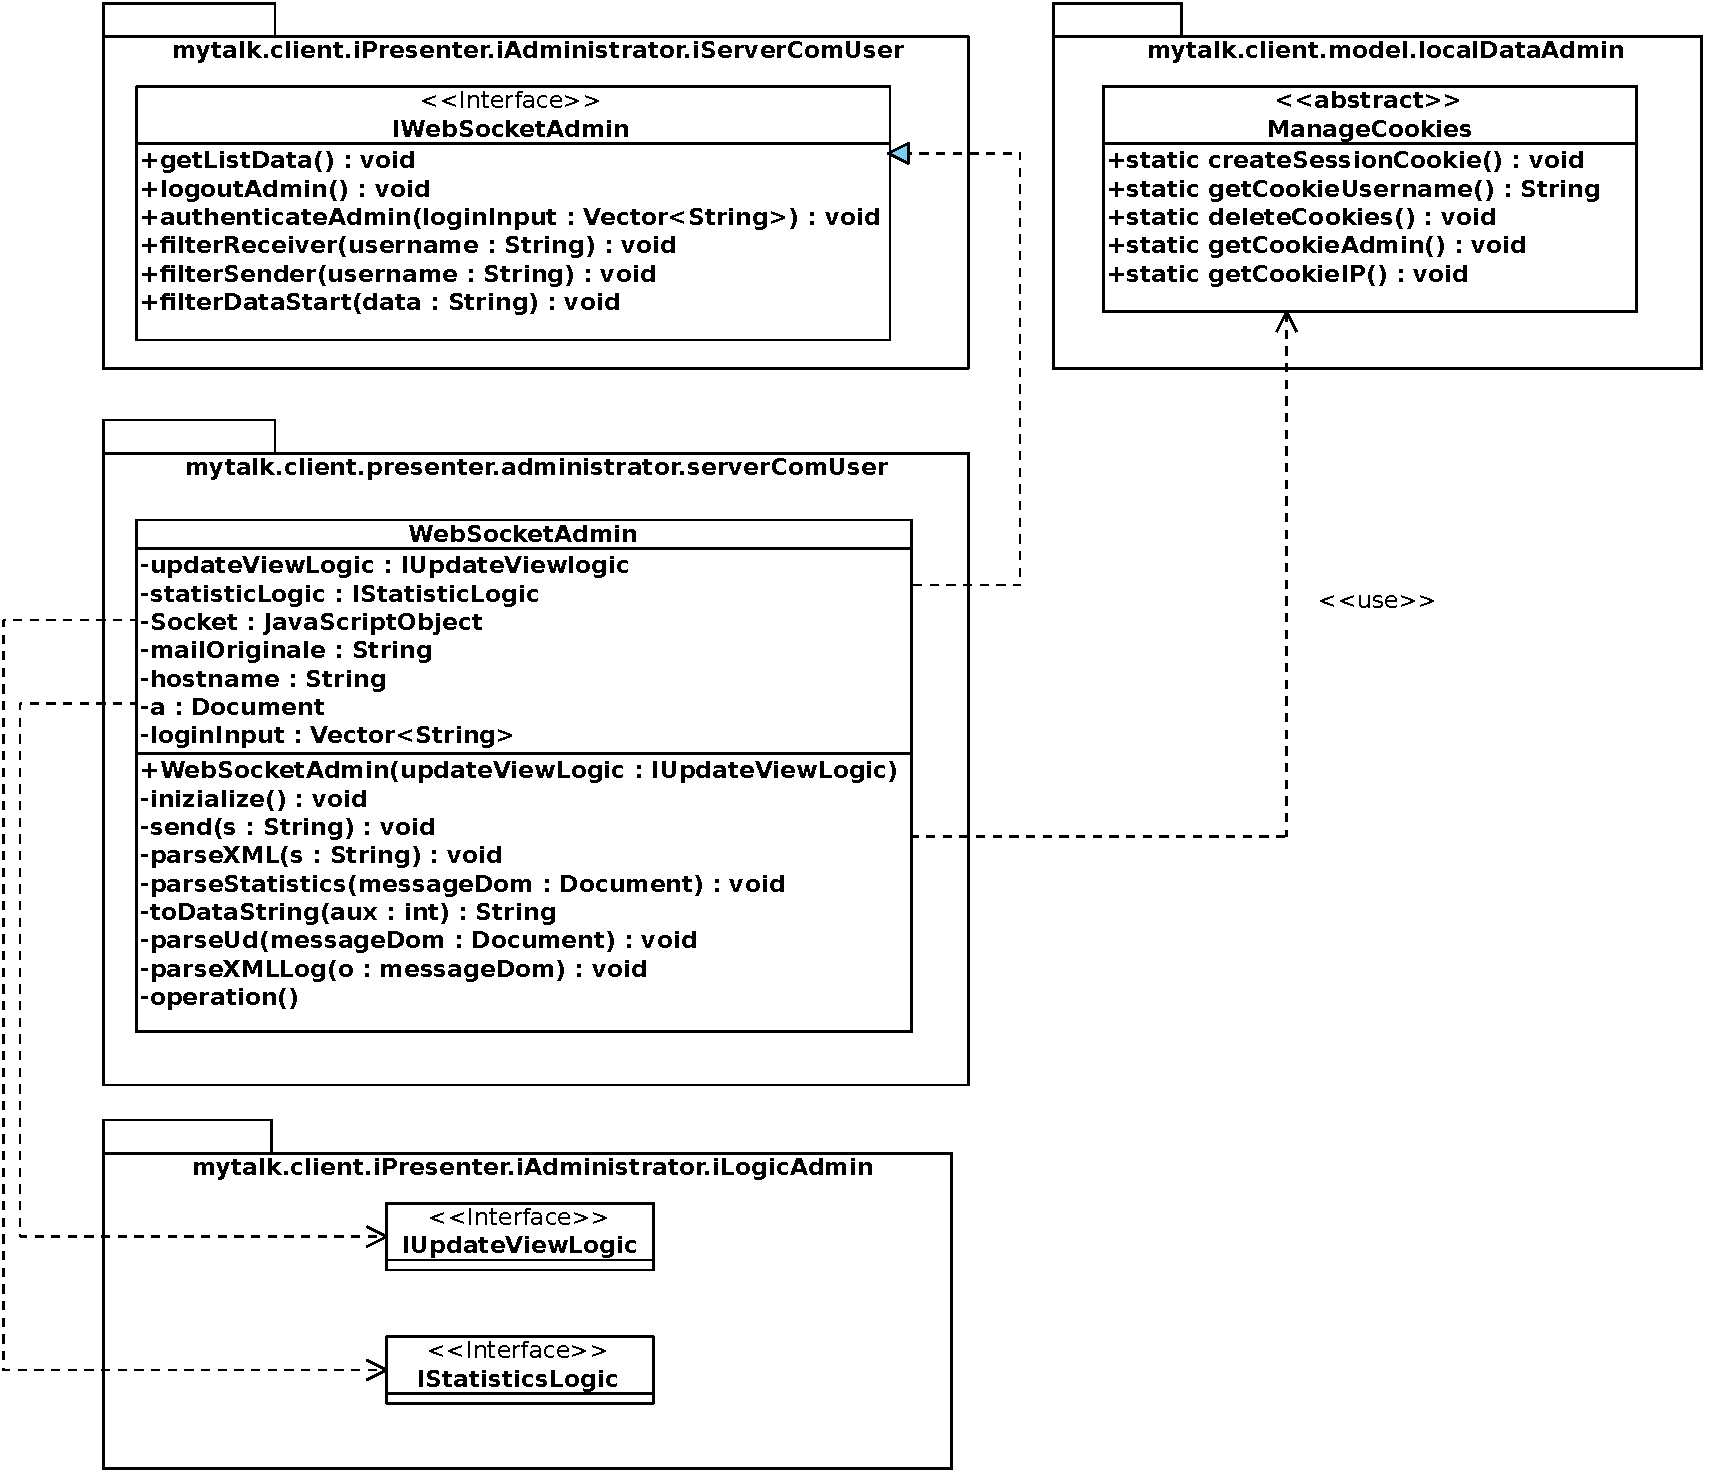
\includegraphics[scale=0.55]{\docsImg classi/presenterClientSocketAdmin.pdf}
\caption{Diagramma delle classi dei package \nolinkurl{mytalk.client.iPresenter.iAdministrator.iServerComAdmin} e  \nolinkurl{mytalk.client.presenter.administrator.serverComAdmin}; dettaglio delle classi \nolinkurl{IWebSocketAdmin} e \nolinkurl{WebSocketAdmin}.}
	\end{figure}	
		
	% IWebSocketAdmin - inizio
		\paragraph{IWebSocketAdmin}\label{par:IWebSocketAdmin}{
			\begin{itemize}
				\item[] \textbf{Funzione:}\\
					L'interfaccia fornisce i metodi tramite i quali è possibile richiedere al server\g~ l'autenticazione di un amministratore e il reperimento delle statistiche.\\
			
				\item[] \textbf{Relazioni con altre componenti:}\\
					L'interfaccia è implementata da:
					\begin{itemize}
						\item[] \path{mytalk.client.presenter.administrator.serverComAdmin.WebSocketAdmin}.
					\end{itemize}
					L'interfaccia è utilizzata da:
					\begin{itemize}
						\item[] \path{mytalkadmin.client.presenter.logicAdmin.StatisticLogic};
						\item[] \path{mytalkadmin.client.presenter.logicAdmin.LogAdminLogic}.\\
					\end{itemize}
			
				\item[] \textbf{Metodi:}{ \\
						\texttt{+ void getListData();}\\
						Richiede l'insieme delle statistiche al server\g.\\
						
						\texttt{+ void logoutAdmin(String data);}\\
						Richiede l'uscita dal servizio da parte dell'amministratore.\\
						
						\texttt{+ void authenticateAdmin(Vector<String> loginInput);}\\
						Richiede l'autenticazione al servizio di amministratore.\\
						
						\texttt{+ void filterSender(String username);}\\
						Richiede le statistiche delle chiamate che coinvolgono un determinato utente chiamante.\\
						
						\texttt{+ void filterDataStart(String data);}\\
						Richiede le statistiche che hanno avuto una determinata data di inizio.\\
						
						\texttt{+ filterGrade(String voto)}\\
						Richiede al server\g~ la lista della statistiche che hanno avuto un determinato giudizio da parte degli utenti.\\
						
						\texttt{+ userList()}\\
						Richiede al server\g~ la lista degli utenti registrati al servizio.\\
						
						\texttt{+ filterGrade(String voto)}\\
						Richiede al server\g~ la lista della statistiche che hanno avuto un determinato giudizio da parte degli utenti. Per far ciò invia un messaggio XML\g~ al server nella forma \ref{opCValStat}.\\
						
						\texttt{- void inizialize()}\\
						Inizializza i campi dati della classe e crea un oggetto di tipo \texttt{WebSocket} che permette di inviare e ricevere messaggi dal server\g.\\
						
						\texttt{- void parseXMLUserList(Document messageDom)}\\
						Viene richiamato per estrapolare nome utente, nome e cognome dalla lista di utenti registrati al server\g~ in formato XML\g~ inviata dal server\g.\\
						Una volta estratta la lista dal messaggio viene richiamato il metodo dell'oggetto \texttt{updateViewLogic} \texttt{setUserList(Vector<String> utenti)} per inviare la lista alla View.\\
						
					
				}
			\end{itemize}
		% IWebSocketAdmin - fine
		}
	}
	
	\subsubsection{Package mytalk.client.presenter.administrator.serverComAdmin}{
	Il diagramma delle classi è contenuto nell'immagine \ref{fig:adminLogicAdmin}.
	
	% WebSocketAdmin - inizio
		\paragraph{WebSocketAdmin}\label{par:WebSocketAdmin}{
			\begin{itemize}
				\item[] \textbf{Funzione:}\\
				la classe ha il compito di gestire la comunicazione con il server\g~ e di richiamare gli opportuni metodi della classe \texttt{UpdateViewLogic} per aggiornare l'interfaccia grafica.\\
			
				\item[] \textbf{Relazioni con altre componenti:}\\
					La classe implementa l'interfaccia:
					\begin{itemize}
						\item[] \path{mytalk.client.iPresenter.iAdministrator.iServerComAdmin.IWebSocketAdmin}.
					\end{itemize}
					La classe utilizza la classe:
					\begin{itemize}
						\item[] \path{mytalk.client.presenter.administrator.logicAdmin.UpdateViewLogic;};
					\end{itemize}
				
				\item[] \textbf{Attributi:}{\\
					\texttt{- IUpdateViewLogic updateViewLogic}: riferimento all'oggetto che ha il compito di aggiornare l'interfaccia GUI\g.\\
					
					\texttt{- JavaScriptObject Socket}: riferimento all'oggetto che rappresenta il WebSocket e che ha la funzione di inviare e ricevere messaggi dal server\g.\\
					
					\texttt{- static String hostname}: stringa che indica il nome dell'host sul quale risiede il WebSocket. Il valore è \texttt{"ws://{IP-address}:8080/MyTalk-server/WSAdmin"}.\\
					
					\texttt{- Document a;}: il tipo Document serve a contenere e verificare la buona formazione della stringa XML\g~ inviata dal server\g.\\
					
					\texttt{- Vector<String> loginInput}: il vettore contiene i dati con i quali l'utente amministratore si è autenticato (o i dati con cui ha tentato di farlo).\\
				}
			
				\item[] \textbf{Metodi:}{ \\
					\texttt{+ WebSocketAdmin(IUpdateViewLogic updateViewLogic)}\\
					Costruttore ad un parametro: richiama il metodo \texttt{inizialize()} dopo aver assegnato il riferimento passatogli come parametro al campo dati \texttt{updateViewLogic}.
					
					\texttt{+ void getListData();}\\
					Il metodo ha lo scopo di richiedere l'insieme delle statistiche al server\g, tramite un messaggio XML\g~ nella forma \ref{opCValStat}.\\
					
					\texttt{+ void logoutAdmin(String data);}\\
					Il metodo ha il compito di richiedere l'uscita dal servizio da parte dell'amministratore, tramite un messaggio XML\g~ nella forma \ref{opUlg}.\\
					
					\texttt{+ void authenticateAdmin(Vector<String> loginInput);}\\
					Il metodo richiede l'autenticazione al servizio di amministratore, tramite un messaggio XML\g~ nella forma \ref{opLog}.\\
					
					\texttt{+ void filterSender(String username);}\\
					Il metodo richiede le statistiche delle chiamate che coinvolgono un determinato utente chiamante, tramite un messaggio XML\g~ nella forma \ref{opCValStat}.\\
					
					\texttt{+ void filterDataStart(String data);}\\
					Il metodo richiede le statistiche che hanno avuto una determinata data di inizio, tramite un messaggio XML\g~ nella forma \ref{opCValStat}.\\
					
					\texttt{- void parseXML(String XML\g~);}\\
					Il metodo riceve come parametro una stringa XML\g~, ne controlla la buona formazione e il contenuto e a seconda di quest'ultimo richiama l'opportuno metodo.\\
					
					\texttt{- void parseStatistics(Document messageDom);}\\
					Il metodo viene richiamato se il messaggio XML\g~ proveniente dal server\g~ contiene delle statistiche. Il metodo prima estrae i valori delle varie statistiche dal messaggio e poi richiama il metodo della classe \texttt{UpdateViewLogic setListData(Vector<Vector<String>> stats)} che invierà i dati all'interfaccia grafica così che possano essere visualizzati.\\
					
					\texttt{- void parseUd(Document messageDom);}\\
					Il metodo viene richiamato se il messaggio XML\g~ proveniente dal server\g~ contiene delle informazioni riguardanti l'autenticazione dell'utente amministratore.\\
					
					\texttt{- void parseXMLLog(Document messageDom);}\\
					Il metodo viene richiamato se si riceve un responso da parte del server\g~ su una richiesta di autenticazione precedentemente inviata dall'utente amministratore.\\
					
					\texttt{+ userList();}\\
						Richiede al server\g~ la lista degli utenti registrati al servizio. Per far ciò invia al server un messaggio nella forma \ref{opCUList}.\\
				}
			\end{itemize}
			}
		% WebSocketAdmin - fine

	}
	
	
	
	\subsubsection{Package mytalk.client.presenter.user.logicUser.common }{
		Il diagramma delle classi è contenuto nell'immagine \ref{fig:presenterLogicUser}.

		% CommonFunctions - inizio
		\paragraph{CommonFunctions}\label{par:CommonFunctions}{
			\begin{itemize}
				\item[] \textbf{Funzione:}{\\
				Classe astratta che contiene metodi di utilità per il controllo delle stringhe che vengono utilizzati in più classi.\\
				}
			
				\item[] \textbf{Relazioni con altre componenti:}{\\
				I suoi metodi vengono richiamati dalle classi:
				\begin{itemize}
					\item[] \path{mytalk.client.presenter.user.logicUser.LogUserLogic};
					\item[] \path{mytalk.client.presenter.user.logicUser.RegisterLogic};
					\item[] \path{mytalk.client.presenter.user.logicUser.DataUserLogic}.\\
				\end{itemize}
				}
				
				\item[] \textbf{Attributi:}{\\
				Nessuno.\\
				}
			
				\item[] \textbf{Metodi:}{ \\
					\texttt{+ static boolean checkEmail(String email);}\\
					Controlla che la mail sia ben formata. Ritorna l'esito di tale controllo.\\
					
					\texttt{+ static boolean ckechPassword(String password);}\\
					Controlla che la password sia di almeno 8 caratteri. Ritorna l'esito di tale controllo.\\
					
					\texttt{+ static boolean checkString(String n);}\\
					Controlla che il parametro ricevuto corrisponda a un nome o un cognome, cioè che sia solo formato da lettere e spazi. Ritorna l'esito di tale controllo.\\
					
					\texttt{+ static boolean checkPasswordControl(String psw, String pswC);}\\
					Controlla che i due parametri \texttt{psw} e \texttt{pswC} siano uguali. Ritorna l'esito di tale controllo.\\
					
					\texttt{+ static boolean checkCompany(String company);}\\
					Controlla che il parametro ricevuto, che corrisponde al nome dell'azienda con il quale l'utente intende registrarsi, non sia formato solo da numeri. Ritorna l'esito di tale controllo.\\
					
					\texttt{+ static boolean checkNumber(String number);}\\
					Controlla che il parametro ricevuto sia un numero telefonico nel formato corretto. Ritorna l'esito di tale controllo.\\
					
					\texttt{+ static void correctInput(Vector<String> userInput);}\\
					Effettua delle correzioni di base sull'input dell'utente: toglie eventuali spazi inutili all'inizio e alla fine delle stringhe e converte l'indirizzo e-mail in minuscolo.
				}
			\end{itemize}
			}
		% CommonFunctions - fine

	}
	
	
		\newpage
		\subsubsection{Package mytalk.client.iPresenter.iUser.iServerComUser}{
		
		\begin{figure}[h!tbp]
		\centering
		\label{fig:presenterUserServerComUser}
		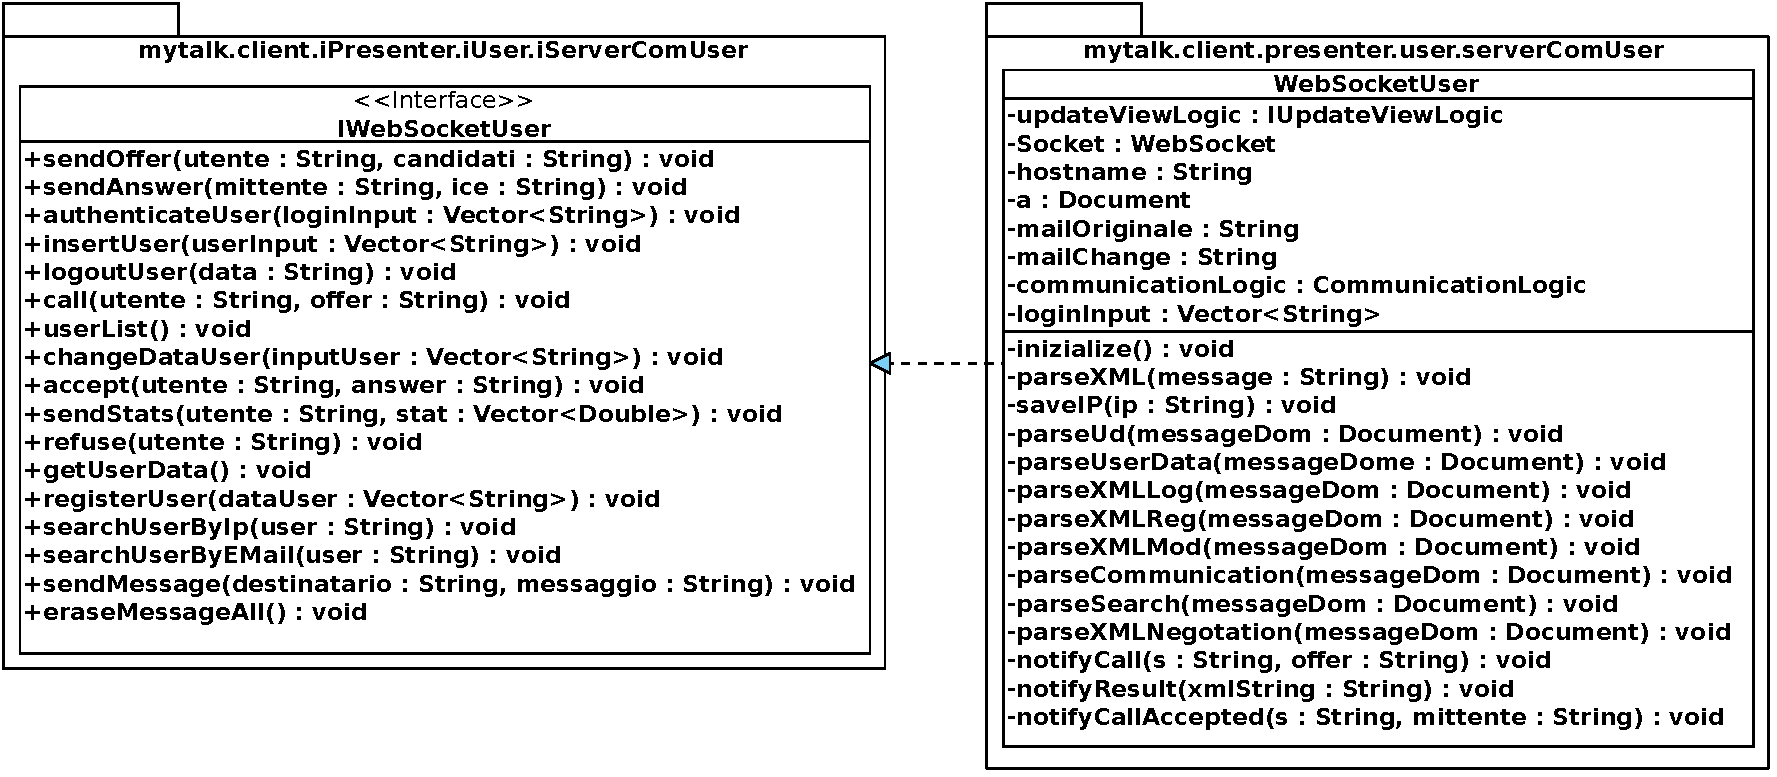
\includegraphics[scale=0.55]{\docsImg classi/socketUser.pdf}
\caption{Diagramma delle classi dei package \nolinkurl{mytalk.client.iPresenter.iUser.iServerComUser} e  \nolinkurl{mytalk.client.presenter.user.serverComUser}; dettaglio delle classi \nolinkurl{IWebSocketUser} e \nolinkurl{WebSocketUser}.}		
	\end{figure}			
		
			
		% IWebSocketUser - inizio
		\paragraph{IWebSocketUser}\label{par:IWebSocketUser}{
			\begin{itemize}
		
				\item[] \textbf{Funzione:}
					le classi che implementano questa interfaccia hanno il compito di comporre ed inviare i messaggi verso il server\g e di ricevere e tradurre i messaggi provenienti dal server\g.\\
			
				\item[] \textbf{Relazioni con altre componenti:}{\\
					L'interfaccia è implementata dalla classe:
					\begin{itemize}
						\item[] \path{mytalk.client.presenter.user.serverComUser.WebSocketUser}.
					\end{itemize}	  
					L'interfaccia è utilizzata da:
					\begin{itemize}
						\item[] \path{mytalk.client.presenter.user.logicUser.LogUserLogic};
						\item[] \path{mytalk.client.presenter.user.logicUser.RegisterLogic};
						\item[] \path{mytalk.client.presenter.user.logicUser.DataUserLogic};
						\item[] \path{mytalk.client.presenter.user.logicUser.CommunicationLogic}.\\
					\end{itemize}
				}
			
				\item[] \textbf{Metodi:}{ \\
				\texttt{+ void accept(String utente, String answer);}\\
				Invia un messaggio al server\g~ che poi verrà recapitato all'utente ricevente se questo è online. Il messaggio indica che l'utente mittente ha accettato la chiamata dell'utente ricevente e fornisce all'utente che ha chiamato la descrizione della sessione locale dell'utente.\\

					\texttt{+ void call(String utente, String offer);}\\
					Invia un messaggio all'utente passato come parametro, il messaggio viene prima inviato al server\g~ e poi da questo viene inviato all'utente ricevente, il messaggio indica che l'utente mittente vuole instaurare una comunicazione con l'utente ricevente e per far ciò fornisce all'utente remoto la descrizione della sessione locale.\\

					\texttt{+ void refuse(String utente);}\\
					Invia un messaggio all'utente passato come parametro. Il messaggio viene prima inviato al server\g~ e poi da questo viene inviato all'utente ricevente. Tale messaggio indica che l'utente mittente ha rifiutato la richiesta di comunicazione dell'utente ricevente.\\

					\texttt{+ void sendOffer(String utente, String iceCandidate);}\\
					Invia un messaggio all'utente passato come parametro. Il messaggio viene prima inviato al server\g~ e poi da questo viene inviato all'utente ricevente. Tale messaggio contiene inoltre gli IceCandidate della sessione dell'utente.\\

					\texttt{+ void sendAnswer(String mittente, JavaScriptObject description);}\\
					Invia un messaggio all'utente passato come parametro. Il messaggio viene prima inviato al server\g~ e poi da questo viene inviato all'utente ricevente. Tale messaggio contiene inoltre gli IceCandidate della sessione dell'utente.\\

					\texttt{+ void changeDataUser(Vector<String> inputUser);}\\
					Invia al server\g~ i nuovi dati personali dell'utente.\\

					\texttt{+ void sendStats(String ricevente, Vector<Double> stats);}\\
					Il metodo, invocato al termine della chiamata invia le statistiche al server\g. Quest'ultimo le memorizza nella base di dati per renderle disponibili agli utenti amministratori.\\

					\texttt{+ void authenticateUser(Vector<String> loginInput);}\\
					Richiede al server\g~ l'autenticazione dell'utente i cui dati di login sono passati come parametro.\\

					\texttt{+ void logoutUser(String data);}\\
					Richiede al server\g~ l'uscita dal servizio dell'utente i cui dati di login sono stati passati come parametro.\\

					\texttt{+ void userList();}\\
					Richiede al server\g~ la lista degli utenti registrati al servizio.\\

					\texttt{+ void getUserData();}\\
					Richiede al server\g~ i dati personali dell'utente autenticato.\\
					
					\texttt{+ void insertUser(Vector<String> dataUser);}\\
					Il metodo ha lo scopo di inviare al server\g~ la richiesta di registrazione di un nuovo utente al servizio.\\
					
					\texttt{+ void searchUserByIP(String ip);}\\
					Il metodo richiede al server di cercare un utente che abbia associato un determinato indirizzo IP\g.\\

					\texttt{+ void searchUserByEmail(String username);}\\
					Il metodo richiede al server di cercare un utente che abbia associato una determinata e-mail.\\
					
					\texttt{+ void sendMessage(String destinatario, String message);}\\
					Invia un messaggio all'utente indicato dalla stringa \texttt{destinatario}.\\
					 
					\texttt{+ void eraseMessageAll();}\\
					Elimina tutti i messaggi della casella di posta dell'utente.\\	
				}
			\end{itemize}
			}
		% IWebSocketUser - fine
		}
		
	\subsubsection{Package mytalk.client.presenter.user.serverComUser}{

% WebSocketUser - inizio
		\paragraph{WebSocketUser}\label{par:WebSocketUser}{
			\begin{itemize}
				\item[] \textbf{Funzione:}\\
					La classe ha il compito di comporre ed inviare i messaggi verso il server\g. Riceve e traduce i messaggi provenienti dal server\g.\\
			
				\item[] \textbf{Relazioni con altre componenti:}{\\
					La classe implementa l'interfaccia:
					\begin{itemize}
						\item \path{mytalk.client.iPresenter.iUser.iServerComUser.IWebSocketUser}.
					\end{itemize}
						La classe è utilizzata da:
					\begin{itemize}
						\item[] \path{mytalk.client.presenter.user.logicUser.LogUserLogic};
						\item[] \path{mytalk.client.presenter.user.logicUser.RegisterLogic};
						\item[] \path{mytalk.client.presenter.user.logicUser.DataUserLogic};
						\item[] \path{mytalk.client.presenter.user.logicUser.CommunicationLogic}.
					\end{itemize}
					Tramite l'interfaccia:
					\begin{itemize}
						\item \path{mytalk.client.iPresenter.iUser.iServerComUser.IWebSocketUser}.\\
					\end{itemize}
				}
				
				\item[] \textbf{Attributi:}{\\
					\texttt{- IUpdateViewLogic updateViewLogic}: riferimento all'oggetto che gestisce gli aggiornamenti della View.\\
					
					\texttt{- JavaScriptObject socket}: riferimento all'oggetto che rappresenta il WebSocket.\\
					
					\texttt{- String hostname}: indirizzo del WebSocket sulla componente server\g.\\
					
					\texttt{- Document a}: documento XML\g~. Tramite questo oggetto viene controllato che il messaggio XML\g~ proveniente dal server\g~ sia ben formato.\\
					
					\texttt{- String MailOriginale}: contiene l'e-mail con la quale l'utente si è autenticato.\\
					
					\texttt{- String MailChange}: contiene l'e-mail la nuova e-mail impostata dall'utente. Se l'utente non ha cambiato l'e-mail in questa sessione il campo è uguale a \texttt{MailOriginale}.\\
					
					\texttt{- ICommunicationLogic communicationLogic}: riferimento all'oggetto che gestisce la comunicazione.\\
					
					\texttt{- Vector<String> loginInput}: contiene i dati con i quali l'utente si è autenticato o ha tentato di farlo.\\
				}
			
				\item[] \textbf{Metodi:}{ \\
					\texttt{+ WebSocketUser(IUpdateViewLogic updateViewLogic);}\\
					Costruttore: riceve come parametro un oggetto di tipo \path{mytalk.client.presenter.user.logicUser.UpdateViewLogic} e con esso inizializza il campo dati \texttt{updateViewLogic}.\\

					\texttt{+ public void inizialize();}\\
					Inizializza il campo dati \texttt{webSocket} e ne registra gli eventi.\\

					\texttt{+ void accept(String utente, String answer);}\\
					Invia un messaggio al server\g~ che poi verrà recapitato all'utente ricevente se questo è online. Il messaggio indica che l'utente mittente ha accettato la chiamata dell'utente ricevente e fornisce al chiamante la descrizione della sessione locale di tipo \texttt{answer} dell'utente codificata in formato JSON\g.\\

					\texttt{+ void call(String utente, String offer);}\\
					Invia un messaggio all'utente passato come parametro. Il messaggio viene prima inviato al server\g~ e poi da questo viene inviato all'utente ricevente. Tale messaggio indica che l'utente mittente vuole instaurare una comunicazione con l'utente ricevente e per far ciò fornisce all'utente remoto la descrizione della sessione locale di tipo \texttt{offer} codificata in formato JSON.\\

					\texttt{+ void refuse(String utente);}\\
					Invia un messaggio all'utente passato come parametro. Il messaggio viene prima inviato al server\g~ e poi da questo viene inviato all'utente ricevente. Tale messaggio indica che l'utente mittente ha rifiutato la richiesta di comunicazione dell'utente ricevente.\\

					\texttt{+ void sendOffer(String utente, String iceCandidate);}\\
					Invia un messaggio all'utente passato come parametro. Il messaggio viene prima inviato al server\g~ e poi da questo viene inviato all'utente ricevente. Tale messaggio contiene inoltre gli IceCandidate della sessione dell'utente.\\

					\texttt{+ void sendAnswer(String mittente, String iceCandidate);}\\
					Invia un messaggio all'utente passato come parametro. Il messaggio viene prima inviato al server\g~ e poi da questo viene inviato all'utente ricevente. Tale messaggio contiene inoltre gli IceCandidate della sessione dell'utente.\\

					\texttt{+ void changeDataUser(Vector<String> inputUser);}
					Invia al server\g~ i nuovi dati personali dell'utente.\\

					\texttt{+ void sendStats(String ricevente, Vector<Double> stats);}\\
					Il metodo, invocato al termine della chiamata, invia le statistiche al server\g~ che poi le memorizzerà nella base di dati per renderle disponibili agli utenti amministratori.\\

					\texttt{+ void authenticateUser(Vector<String> loginInput);}\\
					Richiede al server\g~ l'autenticazione dell'utente i cui dati di login sono passati come parametro.

					\texttt{+ void logoutUser(String data);}\\
					Richiede al server\g~ l'uscita dal servizio dell'utente i cui dati di login sono stati passati come parametro.\\

					\texttt{+ void userList();}\\
					Richiede al server\g~ la lista degli utenti registrati al servizio.\\

					\texttt{+ void getUserData();}\\
					Richiede al server\g~ i dati personali dell'utente autenticato.\\	

					\texttt{- void parseXML(String s);}\\
					Esegue il parsing di una stringa XML\g~ giunta dal server\g~ tramite WebSocket, identificandone il tipo di messaggio dal nodo radice. Il messaggio può essere di tre tipi:
					\begin{enumerate}
						\item \texttt{ip}: riceve l'indirizzo IP\g~ dal server\g\g~.
						\item \texttt{userData}: risponde ad una richiesta di login o di registrazione o di modifica dei dati dell'utente che ha inviato la richiesta.
						\item \texttt{communication}: esegue la negoziazione della chiamata e l'interscambio delle sessioni remote.
					\end{enumerate}
					Il metodo, a seconda del contenuto del nodo radice, richiama un opportuno metodo che avrà il compito di estrarre le informazioni dal messaggio XML\g.\\

					\texttt{- void saveIP(String s);}\\	
					Viene invocato qualora dal server\g~ provenga un messaggio contenente l'indirizzo IP\g~ dell'utente. Viene invocato il metodo della classe \texttt{ManageCookies} per salvare il dato in un cookie\g.\\

					\texttt{- void parseUd(Document messageDom);}\\
					Viene invocato dal metodo \texttt{parseXML} se il messaggio proveniente dal server\g~ contiene informazioni riguardanti:
					\begin{itemize}
						\item[-] login: viene richiamato l'opportuno metodo \texttt{parseXMLLog(Document messageDom)};
						\item[-] registrazione: viene richiamato il metodo \texttt{parseXMLReg(Document messageDom)};
						\item[-] modifica dei dati personali dell'utente: viene richiamato il metodo \texttt{parseXMLMod(Document messageDom)};
						\item[-] dati personali dell'utente: viene richiamato il metodo \texttt{parseUserData(Document messageDom)};\\
					\end{itemize}

					\texttt{- void parseXMLLog(Document o);}\\
					Estrapola l'esito di una richiesta di autenticazione avvenuta in precedenza e richiama il metodo dell'oggetto \texttt{updateViewLogic} \texttt{loginResult(boolean loginSucces, Vector<String> loginInput)} per notificare l'esito all'utente.\\

					\texttt{- void parseXMLReg(Document o);}	\\
					Estrapola l'esito di una richiesta di registrazione avvenuta in precedenza e richiama il metodo dell'oggetto \texttt{updateViewLogic} \texttt{registerResult(boolean registerSuccess} per notificare l'esito all'utente.\\

					\texttt{- void parseXMLMod(Document o);}\\
					Estrapola l'esito di una richiesta di modifica dei dati personali dell'utente avvenuta in precedenza e richiama il metodo dell'oggetto \texttt{updateViewLogic} \texttt{resultDataUser(boolean update)} per notificare l'esito all'utente.\\

					\texttt{- void parseUserData(Document o);}\\
					Estrapola i dati personali dell'utente dal documento XML\g~ passato come parametro. I dati vengono quindi passati al metodo \texttt{setUserDataLabel(Vector<String> dataUser)} dell'oggetto \texttt{updateViewLogic}.\\

					\texttt{- void parseCommunication(Document messageDom);}\\
					Viene invocato dal metodo \texttt{parseXML} se il messaggio proveniente dal server\g~ contiene informazioni riguardanti la parte relativa alla comunicazione. In particolare:
					\begin{itemize}
						\item[-] negoziazione: quando un utente tramite il server\g~ invia un messaggio all'utente che può indicare una chiamata, l'accettazione di una chiamata o il rifiuto di una chiamata. In questi casi viene chiamato il metodo \texttt{parseXMLNegotation(Document messageDom)}.
						\item[-] scambio: quando la chiamata è stata già accettata dall'utente chiamato e l'allacciamento della comunicazione è già in fase avanzato. Questa fase riguarda lo scambio degli IceCandidate e se il messaggio contiene uno o più di questi oggetti viene richiamato il metodo \texttt{parseXMLExchange(Document messageDom)}.
						\item[-] ricerca: contiene il responso che il server\g~ fornisce in seguito alla richiesta di un utente di chiamare o digitando il nome dell'utente ricevente o il suo indirizzo IP\g~ e non di selezionarlo dalla lista di quelli registrati al server\g. Per estrapolare l'esito della ricerca viene richiamato il metodo \texttt{- void parseSearch(Document messageDom)}. 
						\item[-] richiesta lista utenti: contiene la lista degli utenti registrati al server\g. Per estrapolare l'esito della ricerca viene richiamato il metodo \texttt{parseXMLUserList(Document messageDom)}.\\
					\end{itemize}

					\texttt{- void parseSearch(Document messageDom);}\\
					Estrapola il nome utente fornito dal server\g~ o notifica l'esito negativo della ricerca alla componente grafica. Se la ricerca ha avuto successo allora viene chiamato l'utente corrispondente tramite il metodo \texttt{call(String utente)} dell'oggetto \texttt{communicationLogic}.\\

					\texttt{- void parseXMLNegotation(Document r);}\\
					A seconda che si tratti di un'offerta (una chiamata in entrata) o di una risposta (l'indicazione dell'accettazione o meno della comunicazione da parte dell'altro utente) richiama il metodo \texttt{notifyCall(String user, String offer)} se si tratta di una chiamata in entrata o \texttt{notifyResult(String user)} se si tratta del responso di una precedente richiesta.\\

					\texttt{- void notifyCall(String s, String offer);}\\
					Viene richiamato per notificare una chiamata in arrivo all'utente ed, eventualmente, per impostare la descrizione remota proveniente dall'utente chiamante. Richiama i metodi \texttt{callEnter(String offer)} dell'oggetto \texttt{communicationLogic} e \texttt{notifyCall(String utente)} dell'oggetto \texttt{updateViewLogic}.\\

					\texttt{- void notifyResult(Document messageDom);}\\
					Estrapola l'accettazione o il rifiuto dell'utente chiamato dal messaggio XML\g~ proveniente dal server\g~. Se il messaggio è di accettazione viene estratta anche la descrizione remota di tipo \texttt{answer}, che deve essere quindi presente e viene richiamato il metodo \texttt{notifyCallAccepted(String answer, String mittente)} al quale vengono inviati come parametri la descrizione di sessione remota e il nome dell'utente che ha inviato il messaggio. Se il messaggio è di rifiuto viene richiamato il metodo \texttt{notifyCallRefused(String mittente)} al quale viene passato come parametro il nome dell'utente che ha inviato il messaggio.\\

					\texttt{- void notifyCallAccepted(String answer, String mittente);}\\
					Notifica alla classe \texttt{CommunicationLogic} l'accettazione della chiamata da parte dell'utente chiamato. Per la notifica viene richiamato il metodo \texttt{acceptedCall(answer, mittente)}.\\

					\texttt{- void notifyCallRefused(String mittente);}\\
					Notifica alla classe \texttt{UpdateViewLogic} il rifiuto della chiamata da parte dell'utente chiamato. Per la notifica viene richiamato il metodo \texttt{refusedCall(mittente)}.\\

					\texttt{- void parseXMLUserList(Document messageDom);}\\
					Il metodo viene richiamato per estrapolare il nome utente, nome e cognome dalla lista di utenti registrati al server\g~ in formato xml\g~ inviata dal server\g.\\
					Una volta estratta la lista dal messaggio viene richiamato il metodo dell'oggetto \texttt{updateViewLogic} \texttt{setUserList(Vector<String> utenti)} per inviare la lista alla View.\\

					\texttt{- void parseXMLExchange(Document messageDom);}\\
					Il metodo viene richiamato quando vengono ricevuti gli \texttt{IceCandidate} da parte dell'altro utente. Gli \texttt{IceCandidate} vengono estratti dal messaggio proveniente dal server\g~ e se l'utente che gli ha inviati è quello che ha iniziato la chiamata, viene richiamato il metodo \texttt{receivedOffer(String mittente, Vector<String> iceCandidate)}. Se invece l'utente che ha inviato il messaggio è quello che ha accettato la chiamata, viene richiamato il metodo \texttt{receivedResponse(iceCandidate)}.\\

					\texttt{- void receivedOffer(String mittente, Vector<String> candidate);}\\
					Notifica il ricevimento degli IceCandidate alla classe \texttt{CommunicationLogic} richiamando il metodo \texttt{receivedSession(String mittente, Vector<String> candidate)} dell'oggetto \texttt{communicationLogic}.\\

					\texttt{- void receivedResponse(String mittente, Vector<String> candidate);}\\
					Il metodo notifica il ricevimento degli IceCandidate alla classe \texttt{CommunicationLogic} richiamando il metodo \texttt{receivedSessionPerformed(Vector<String> candidate)} dell'oggetto \texttt{communicationLogic}.\\
					
					\texttt{+ void insertUser(Vector<String> dataUser);}\\
					Invia al server la richiesta di registrazione di un nuovo utente al servizio, per far ciò invia al server\g~ un messaggio XML\g~ nella forma \ref{opUReg} utilizzando le stringhe presenti nel vettore passato come parametro.\\
					
					\texttt{+ void searchUserByIP(String ip);}\\
					Richiede al server\g~ di cercare un utente che abbia associato un determinato indirizzo IP\g~. Per far ciò invia un messaggio XML\g~ al server\g~ nella forma \ref{opCEus}.\\

					\texttt{+ void searchUserByEmail(String username);}\\
					Richiede al server di cercare un utente che abbia associato un determinato indirizzo e-mail. Per far ciò invia al server\g~ un messaggio XML\g~ nella forma \ref{opCEus}.\\
					
					\texttt{+ void sendMessage(String destinatario, String message);}\\
					Invia, grazie al server, un messaggio all'utente indicato dalla stringa \texttt{destinatario}.\\
					 
					\texttt{+ void eraseMessageAll();}\\
					Elimina, grazie al server, tutti i messaggi della casella di posta dell'utente.\\	
				}
			\end{itemize}
			}
		% WebSocketUser - fine

	}


	\subsection{Server}{\label{presenter.server}

	La sotto-componente Server\g~ gestisce le comunicazioni ricevute ed inviate dalla sotto-componente Client\g~ (vedi \ref{presenter.client}). A questo scopo interroga la sotto-componente Server\g~ del Model (vedi \ref{model.server}) e compone i messaggi XML\g~ risultato (vedi  \ref{par:XMLComm}).\\
	\`E composta dalle classi:
	\begin{itemize}
		\item[] \texttt{mytalk.server.presenter.XMLField} (sez. \ref{par:XMLField})\\

		\item[] \texttt{mytalk.server.presenter.administrator.logicAdmin.IWSAdmin} (sez. \ref{par:IWSAdmin})
		\item[] \texttt{mytalk.server.presenter.administrator.logicAdmin.IManageWSA} (sez. \ref{par:IManageWSA})
		\item[] \texttt{mytalk.server.presenter.administrator.logicAdmin.WSAdmin} (sez. \ref{par:WSAdmin})
		\item[] \texttt{mytalk.server.presenter.administrator.logicAdmin.WSAdmin.WebSocket} (sez. \ref{par:WSAdminWebSocket})
		\item[] \texttt{mytalk.server.presenter.administrator.logicAdmin.ManageWSA} (sez. \ref{par:ManageWSA})
		\item[] \texttt{mytalk.server.presenter.user.logicUser.IWSUser} (sez. \ref{par:IWSUser})
		\item[] \texttt{mytalk.server.presenter.user.logicUser.IManageWSU} (sez. \ref{par:IManageWSU})
		\item[] \texttt{mytalk.server.presenter.user.logicUser.WSUser} (sez. \ref{par:WSUser})
		\item[] \texttt{mytalk.server.presenter.user.logicUser.WSUser.WebSocket} (sez. \ref{par:WSUserWebSocket})
		\item[] \texttt{mytalk.server.presenter.user.logicUser.ManageWSU} (sez. \ref{par:ManageWSU})
	\end{itemize}

	\subsubsection{Package mytalk.server.presenter}{
	
		\begin{figure}[h!tbp]
		\centering
		\label{fig:presenterXMLField}
		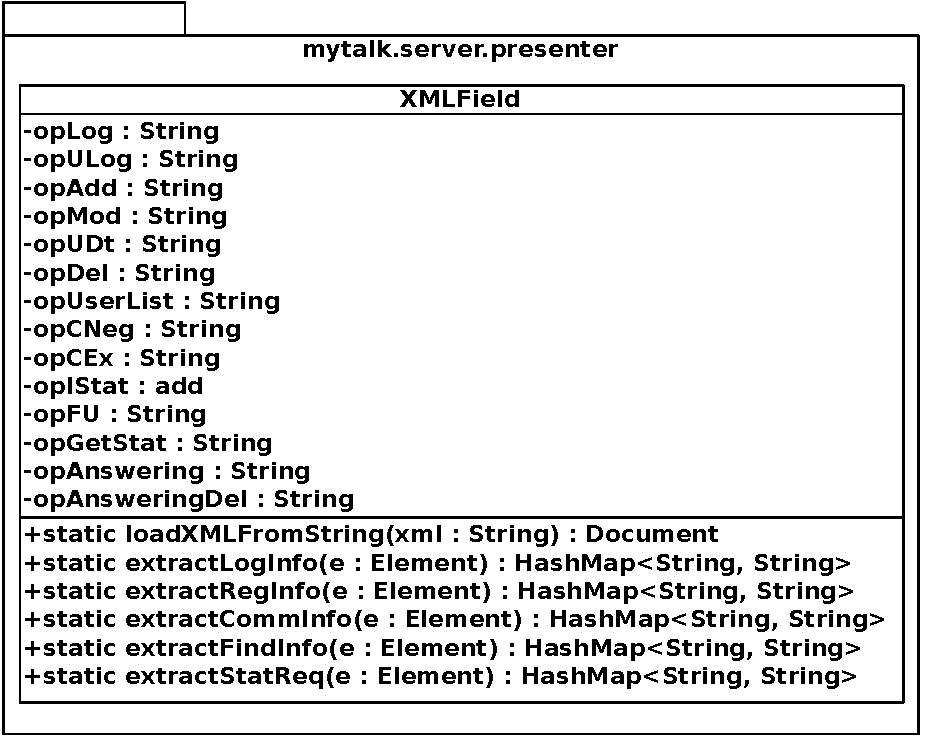
\includegraphics[scale=0.7]{\docsImg classi/serverPresenter.pdf}
\caption{Diagramma delle classi del package \nolinkurl{mytalk.server.presenter}; dettaglio della classe \nolinkurl{XMLField}.}		
	\end{figure}	
		
		% XMLField - inizio
		\paragraph{XMLField}\label{par:XMLField}{
			\begin{itemize}
			\item[] \textbf{Funzione:}\\
				La classe ha lo scopo di raccogliere tutti i metodi e gli attributi utili per l'estrazione delle informazioni nei messaggi in formato XML\g~ pervenuti dal client\g. Le informazioni estrapolate vengono convertite in un formato gestibile dalle classi del package \texttt{mytalk.server.model}.\\
			
			\item[] \textbf{Relazioni con altre componenti:}\\
				Usa le classi:
				\begin{itemize}
					\item[] \path{mytalk.server.model.dao.DataAccessObject};
					\item[] \path{mytalk.server.model.dao.ObjectTransfer}.
				\end{itemize}
				tramite l'interfaccia:
				\begin{itemize}
					\item[] \path{mytalk.server.model.dao.IDataAccessObject};
					\item[] \path{mytalk.server.model.dao.IObjectTransfer};\\
				\end{itemize}
				
				\item[] \textbf{Attributi:}{\\
					\texttt{+ static final String opLog}: identificativo stringa dell'operazione di login nei messaggi XML\g.\\
					
					\texttt{+ static final String opULog}: identificativo stringa dell'operazione di logout nei messaggi XML\g.\\
					
					\texttt{+ static final String opAdd}: identificativo stringa dell'operazione di aggiunta nei messaggi XML\g.\\
					
					\texttt{+ static final String opMod}: identificativo stringa dell'operazione di modifica nei messaggi XML\g.\\
					
					\texttt{+ static final String opUDt}: identificativo stringa dell'operazione per ottenere i dati utente nei messaggi XML\g.\\
					
					\texttt{+ static final String opDel}: identificativo stringa dell'operazione di eliminazione nei messaggi XML\g.\\
					
					\texttt{+ static final String opUserList}: identificativo stringa dell'operazione per ottenere la lista degli utenti nei messaggi XML\g.\\
					
					\texttt{+ static final String opCNeg}: identificativo stringa dell'operazione di negoziazione della comunicazione nei messaggi XML\g.\\
					
					\texttt{+ static final String opCEx}: identificativo stringa dell'operazione di scambio dati della comunicazione nei messaggi XML\g.\\
					
					\texttt{+ static final String opIStat }: identificativo stringa dell'operazione per l'inserimento dati statistici delle comunicazioni nei messaggi XML\g.\\
					
					\texttt{+ static final String opFU}: identificativo stringa dell'operazione di ricerca utente nei messaggi XML\g.\\
					
					\texttt{+ static final String opGetStat}: identificativo stringa dell'operazione di richiesta informazioni statistici.\\
					
					\texttt{+ static final String opAnswering}: identificativo stringa dell'operazione di inserimento nuovo messaggio di segreteria.\\
					
					\texttt{+ static final String opAnsweringDelete}: identificativo stringa dell'operazione di rimozione dei  messaggi in segreteria.\\
					
					\texttt{+ static final HashMap<String, String> reference}: raccolta di riferimenti per i nodi XML\g.\\
					}
			
				\item[] \textbf{Metodi:}{\\
					\texttt{+ static Document loadXMLFromString(String xml) throws Exception};\\
					Gestisce la lettura della stringa XML\g~ (data dal parametro \texttt{xml}) e la converte in una struttura dati \texttt{Document} che facilita, per la VM Java\g~, la lettura delle informazioni dei nodi e la manipolazione di questi.
					Se la lettura della stringa XML\g~ fallisce, il metodo solleva una generica eccezione \texttt{Exception}.\\
					
					\texttt{+ static HashMap<String, String> extractLogInfo(Element e)};\\
					Estrapola i dati di login dell'utente e ne restituisce i valori associati. Il parametro \texttt{e} è una struttura dati contenente i valori estratti dalla stringa XML\g~ originaria.
					La tabella Hash di ritorno contiene i valori, associati a riferimenti specifici, utili per la gestione e la verifica dei dati di login.\\
					
					\texttt{+ static HashMap<String, String> extractRegInfo(Element e)};\\
					Estrapola i dati di registrazione dell'utente e ne restituisce i valori associati.
					Il parametro \texttt{e} è una struttura dati contenente i valori estratti dalla stringa XML\g~ originaria.
					La tabella Hash di ritorno contiene i valori, associati a riferimenti specifici, utili per la gestione e verifica dei dati di registrazione.\\
					
					\texttt{+ static HashMap<String, String> extractCommInfo(Element e)};\\
					Estrapola i dati statistici della comunicazione avvenuta tra gli utenti e ne restituisce i valori associati.
					Il parametro in ingresso \texttt{e} è una struttura dati contenente i valori estratti dalla stringa XML\g~ originaria.
					La tabella Hash di ritorno contiene i valori, associati a riferimenti specifici, utili per la gestione e verifica dei dati statistici della comunicazione.\\
					
					\texttt{+ static HashMap<String, String> extractFindInfo(Element e)};\\
					Estrapola i dati di ricerca dell'utente e ne restituisce i valori associati.
					Il parametro in ingresso \texttt{e} è una struttura dati contenente i valori estratti dalla stringa XML\g~ originaria.
					La tabella Hash di ritorno contiene i valori, associati a riferimenti specifici, utili per la gestione e verifica dei dati di ricerca.\\
					
					\texttt{+ static HashMap<String, String> extractStatReq(Element e)};\\
					Estrapola i dati di ricerca per ottenere i valori statistici richiesti.\\
					Il parametro in ingresso \texttt{e} è una struttura dati contenente i valori estratti dalla stringa XML\g~ originaria.
					La tabella Hash di ritorno contiene i valori, associati a riferimenti specifici, utili per la gestione e verifica dei dati di ricerca.\\
					
				}	
			\end{itemize}
		}
		% XMLField - fine

	}
\newpage
	\subsubsection{Package mytalk.server.presenter.administrator.logicAdmin}{
	
		\begin{figure}[h!tbp]
		\centering
		\label{fig:presenterServerAdmin}
		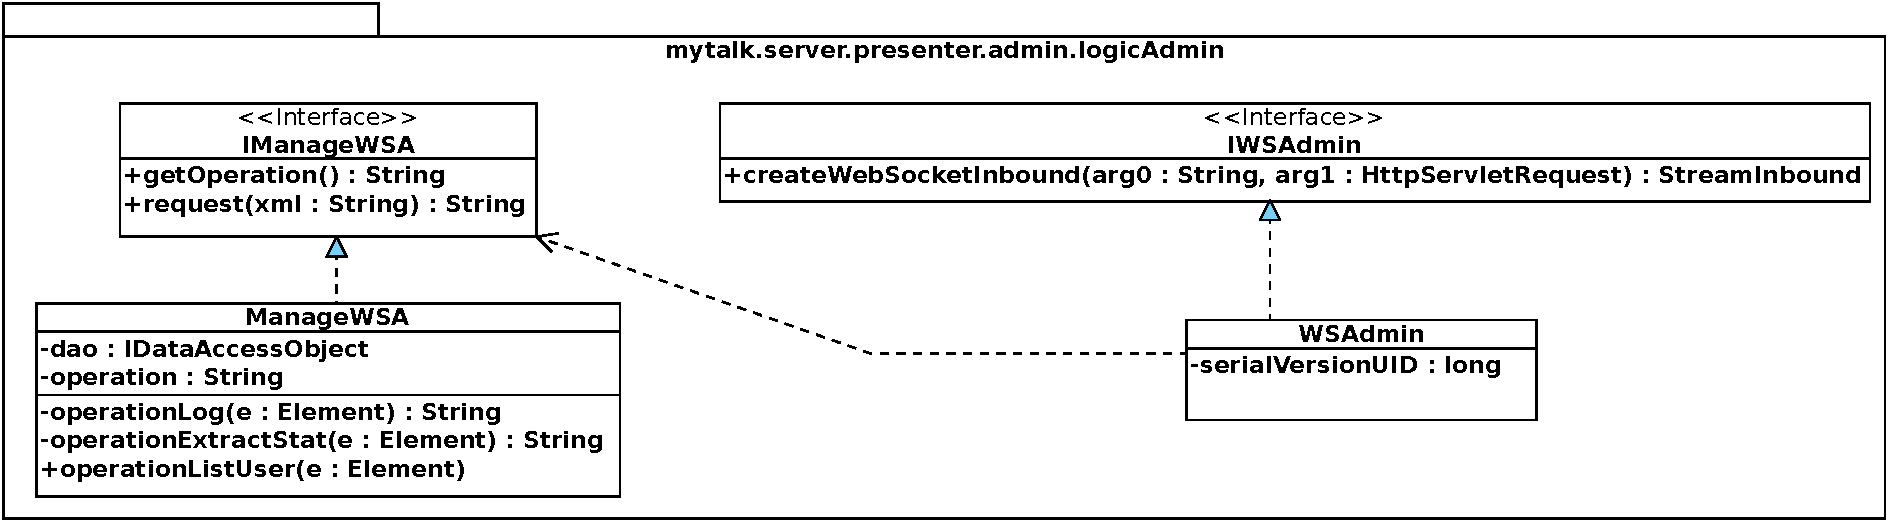
\includegraphics[scale=0.55]{\docsImg classi/serverPresenterAdmin.pdf}
\caption{Diagramma delle classi del package \nolinkurl{mytalk.server.presenter.administrator.logicAdmin}; dettaglio delle classi \nolinkurl{IWSAdmin}, \nolinkurl{IManageWSA}, \nolinkurl{WSAdmin} e  \nolinkurl{ManageWSA}.}		
		%\caption{Diagramma delle classi dettagliato che illustra il package \nolinkurl{mytalk.server.presenter.administrator.logicAdmin} e relazioni con altre componenti.}
	\end{figure}	
	

		
		% IWSAdmin - inizio
		\paragraph{IWSAdmin}\label{par:IWSAdmin}{
			\begin{itemize}
			\item[] \textbf{Funzione:}\\
				Interfaccia che gestisce le connessioni da parte dei Client\g~ di tipo amministratore e mantiene attivo il riferimento per l'ingresso e l'uscita di messaggi da/per il client\g.\\
			
				\item[] \textbf{Relazioni con altre componenti:}\\
					L'interfaccia è implementata da:
					\begin{itemize}
						\item[]	\path{mytalk.server.presenter.administrator.logicAdmin.WSAdmin}.\\
					\end{itemize}
			
				\item[] \textbf{Metodi:}\\
					\texttt{+ createWebSocketInbound(String arg0, HttpServletRequest arg1);}\\
					Ad ogni sua invocazione, crea l'oggetto \texttt{WSAdmin.WebSocket}.\\
			\end{itemize}
		}
		% IWSAdmin - fine
		
		

		% IManageWSA - inizio
		\paragraph{IManageWSA}\label{par:IManageWSA}{
			\begin{itemize}
			\item[] \textbf{Funzione:}\\
					Interfaccia che gestisce i messaggi inviati dall'utente amministratore elaborandoli ed estrapolandone le informazioni di ricerca per poi restituire un messaggio, correttamente composto, al medesimo utente.\\
			
				\item[] \textbf{Relazioni con altre componenti:}{\\
					L'interfaccia è implementata da:
					\begin{itemize}
						\item[]	\path{mytalk.server.presenter.administrator.logicAdmin.ManageWSA}.\\
					\end{itemize}
					}
			
				\item[] \textbf{Metodi:}{ \\
					\texttt{+ String getOperation();}\\
					Ritorna il nome dell'ultima elaborazione effettuata dall'oggetto.\\
					
					\texttt{+ String request(String xml);}\\
					Elabora la stringa in ingresso selezionando l'operazione associata da eseguire (quella richiesta dal messaggio) restituendo il messaggio risultante.\\
				}
				\end{itemize}
		}%IManageWSA



		% WSAdmin - inizio
		\paragraph{WSAdmin}\label{par:WSAdmin}{
			\begin{itemize}
				\item[] \textbf{Funzione:}\\
					La classe serve da riferimento per le comunicazioni \underline{client-server}\g~ per gli utenti di tipo amministratore. Deve inoltre creare l'oggetto \texttt{logicAdmin.WebSocket} per l'invio e ricezione delle comunicazioni.\\
		
				\item[] \textbf{Relazioni con altre componenti:}\\
					Implementa l'interfaccia: 
						\begin{itemize}
							\item[] \path{mytalk.server.presenter.administrator.logicAdmin.IWSAdmin}.
						\end{itemize}
					Usa le classi:
						\begin{itemize}
							\item[] \path{mytalk.server.presenter.administrator.logicAdmin.ManageWSA};
						\end{itemize}
					tramite l'interfaccia:
						\begin{itemize}
							\item[]\path{mytalk.server.presenter.administrator.logicAdmin.IManageWSA}.
						\end{itemize}
					Crea la classe:
						\begin{itemize}
							\item[]\path{mytalk.server.presenter.administrator.logicAdmin.WSAdmin.WebSocket}.\\
						\end{itemize}
				
				\item[] \textbf{Attributi:}\\
					\texttt{- static final long serialVersionUID}: Valore per la classe seriale.\\
			
				\item[] \textbf{Metodi:}{\\
				\texttt{+ StreamInbound createWebSocketInbound(String arg0, HttpServletRequest arg1);}\\
					Gestisce le richieste di connessione pervenute dai client\g~ amministratori.
					Il parametro \texttt{arg0} serve a specificare un sub-protocollo di comunicazione tra client\g~ e server\g. Se non specificato, il suo valore è \texttt{null}.
					Il parametro \texttt{arg1} serve a riferire la richiesta HTTP\g~ catturata che identifica la comunicazione.
					Quando perviene la comunicazione dal client\g~ amministratore, il metodo crea e ritorna un nuovo oggetto \path{WSAdmin.WebSocket} rimanendo accessibile per nuove richieste di connessione.\\
				}
			\end{itemize}
		% WSAdmin - fine
		}
		
		

		% WSAdmin.WebSocket - inizio
		\paragraph{WSAdmin.WebSocket}\label{par:WSAdminWebSocket}{
			\begin{itemize}

				\item[] \textbf{Funzione:}{\\
					La classe ha il compito di gestire le comunicazioni in entrata ed uscita tra i client\g~ di tipo amministratore ed il server\g.
					Quando riceve un nuovo messaggio da parte del client\g~ amministratore, la classe inoltra la stringa alle classi interpreti e queste ultime, in casi specifici, ritornano dei messaggi da inviare al client\g~ amministratore.\\
				 }
				
				\item[] \textbf{Attributi:}\\
					\texttt{- WsOutbound outbound}: riferimento al client\g~ amministratore destinatario del messaggio da inviare.\\
					
					\texttt{- IManageWSA adminManage}: riferimento all'oggetto \path{mytalk.server.presenter.administrator.logicAdmin.IManageWSA} per l'interpretazione dei messaggi in ingresso e creazione dei messaggi d'invio.\\
			
				\item[] \textbf{Metodi:}{\\
					\texttt{\# WebSocket();}\\
					Costruttore: crea il riferimento all'attributo \texttt{adminManage} verso l'oggetto  \path{mytalk.server.presenter.administrator.logicAdmin.ManageWSA}.\\
	
					\texttt{- void sendMessage(WsOutbound o, String m);}\\
					Si occupa dell'invio dei messaggi all'utente amministratore. 
					Il parametro \texttt{o} è un riferimento all'utente amministratore destinatario. Se il valore è \texttt{null}, l'utente al quale viene inviato il messaggio è lo stesso che ha instaurato la connessione specificato dall'attributo \texttt{outbound}.\\
					Il parametro \texttt{m} è un messaggio da inviare all'utente amministratore.\\
				
					\texttt{+ void onOpen(WsOutbound outbound);}\\
					Gestisce la richiesta di aprire una nuova connessione da parte dell'utente amministratore.
					Il parametro \texttt{outbound} è il riferimento all'utente amministratore che ha effettuato la connessione.\\
				
					\texttt{+ void onTextMessage(CharBuffer buffer) throws IOException;}\\
					Gestisce i messaggi inviati dal client\g~ amministratore restituendo un opportuno messaggio quando previsto.
					Il parametro \texttt{buffer} riferisce il contenuto testuale del messaggio.
					Il metodo inoltra il messaggio all'oggetto \path{mytalk.server.presenter.administrator.logicAdmin.ManageWSA}, riferito da \texttt{adminManage}, il quale elabora, verifica e ritorna le informazioni richieste dal messaggio.\\
				}
			\end{itemize}
		%WSAdmin.WebSocket - fine
		}
	
	

		% ManageWSA - inizio
		\paragraph{ManageWSA}\label{par:ManageWSA}{
			\begin{itemize}
				\item[] \textbf{Funzione:}\\
					La classe ha la funzione di gestire le stringhe di messaggi ricevute in ingresso.
					Ciascun messaggio deve avere una struttura basata su sintassi XML\g~ prefissata così da poterne creare una struttura dati ordinata dalla quale estrapolare in modo agevole le informazioni.
					Le informazioni ottenute servono come parametri vincolanti per ottenere informazioni dal DAO per poi essere organizzate in messaggi, sempre in sintassi XML\g~, da inviare al client\g~ amministratore.\\
			
				\item[] \textbf{Relazioni con altre componenti:}{\\			
					Implementa l'interfaccia:
						\begin{itemize}
							\item[] \path{mytalk.server.presenter.administrator.logicAdmin.IManageWSA}.
						\end{itemize}
					Usa le classi:
						\begin{itemize}
							\item[] \path{mytalk.server.presenter.XMLField};
							\item[] \path{mytalk.server.model.dao.DataAccessObject};
							\item[] \path{mytalk.server.model.dao.ObjectTransfert}.
						\end{itemize}
					tramite l'interfaccia:
						\begin{itemize}
							\item[]	\path{mytalk.server.model.dao.IDataAccessObject};
							\item[] \path{mytalk.server.model.dao.IObjectTransfert}.\\
						\end{itemize}
				}
				
				\item[] \textbf{Attributi:}{\\
					\texttt{- static IDataAccessObject dao}: riferimento all'oggetto \path{mytalk.server.model.dao.DataAccessObject} che gestisce le comunicazioni con la base dati.\\
					
					\texttt{- String operation}: riferimento al valore dell'ultima operazione effettuata.\\
				}
			
				\item[] \textbf{Metodi:}{\\
					\texttt{+ String getOperation();}\\
					Metodo getter, ritorna il valore contenuto nell'attributo \texttt{operation}, ovvero, l'ultima operazione gestita dall'oggetto.\\	
					
					\texttt{+ String request(String xml);}\\
					Elabora la stringa XML\g~ fornita in ingresso.
					L'elaborazione della stringa XML\g~ richiede la creazione di una struttura dati ordinata che ne consenta un'agile estrazione delle informazioni; tali informazioni servono poi per scegliere il metodo interno relativo all'operazione richiesta.
					Come risultato, il metodo ritorna una nuova stringa in formato XML\g~ contente le informazioni richieste.\\
					
					\texttt{- String operationLog(Element e);}\\
					Gestisce i dati di login dell'utente amministratore. Il parametro \texttt{e} riferisce la struttura dati che gestisce le informazioni da verificare.
					Una volta fatta l'interrogazione all'oggetto di tipo \path{mytalk.server.model.dao.DataAccessObject}, aggiornandone i valori, il metodo compila il messaggio XML\g~ con le informazioni ricavate.\\

					\texttt{- String operationListUser(Element e);}\\
					Gestisce la richiesta di ottenimento della lista di tutti gli utenti registrati. Il parametro \texttt{e} riferisce la struttura dati che gestisce le informazioni da verificare.
					Una volta fatta l'interrogazione all'oggetto di tipo \texttt{mytalk.server.model.dao.DataAccessObject}, il metodo compila il messaggio XML\g~ con le informazioni ricavate.\\
					
					\texttt{- String operationExtractStat(Element e);}\\
					Gestisce i dati di ricerca delle statistiche di comunicazione. Il parametro \texttt{e} riferisce la struttura dati che gestisce le informazioni da verificare.
					Una volta fatta l'interrogazione all'oggetto di tipo \texttt{mytalk.server.model.dao.DataAccessObject}, il metodo compila il messaggio XML\g~ con le informazioni ricavate.\\
					
					\texttt{- String operationListUser(Element e);}\\
					Gestisce la richiesta di ottenimento della lista di tutti gli utenti registrati. Il parametro \texttt{e} riferisce la struttura dati che gestisce le informazioni da verificare.
					Una volta fatta l'interrogazione all'oggetto di tipo \path{mytalk.server.model.dao.DataAccessObject}, il metodo compila il messaggio XML\g~ con le informazioni ricavate.\\
				}
			\end{itemize}
		% ManageWSA - fine
		}
	}
	%mytalk.server.presenter.administrator.logicAdmin
	
	
	\subsubsection{Package mytalk.server.presenter.user.logicUser}{
	
		\begin{figure}[h!tbp]
		\centering
		\label{fig:presenterServerUser}
		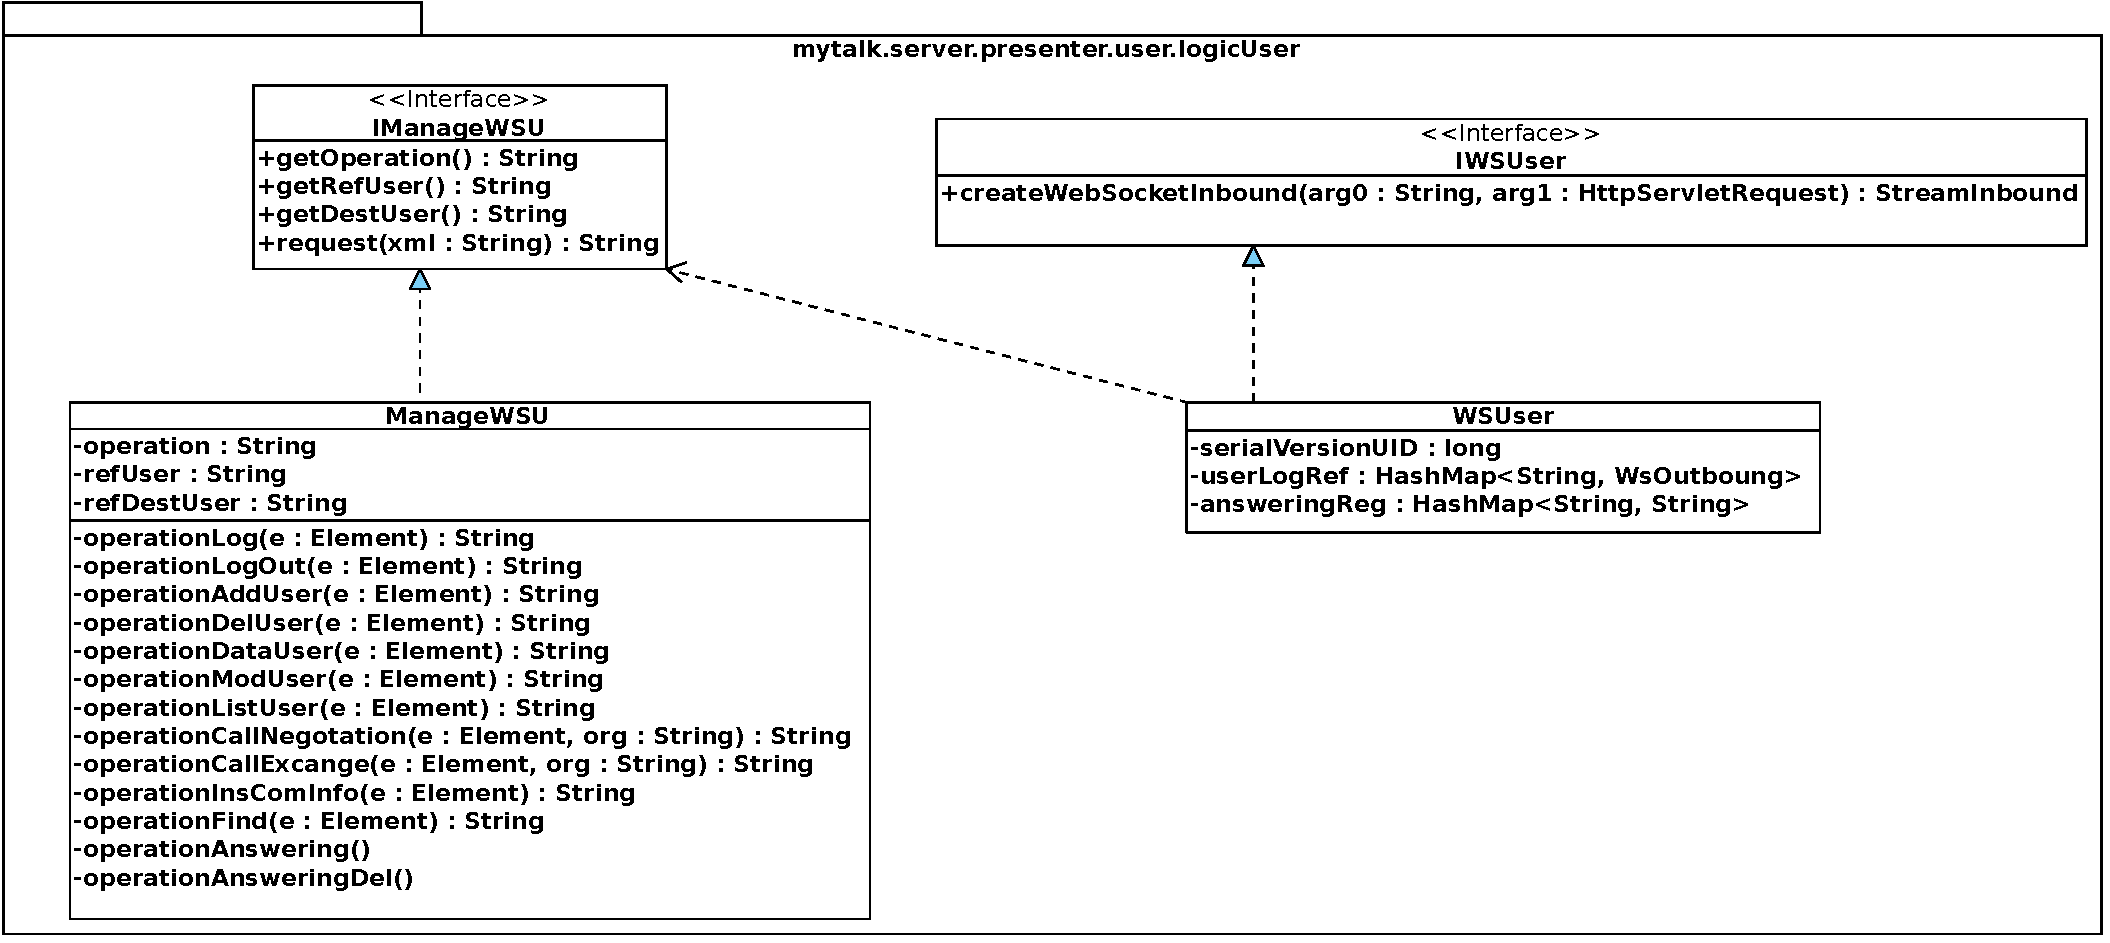
\includegraphics[scale=0.5]{\docsImg classi/serverPresenterUser.pdf}
		\caption{Diagramma delle classi del package \nolinkurl{mytalk.server.presenter.user.logicUser}; dettaglio delle classi \nolinkurl{IWSUser}, \nolinkurl{IManageWSU}, \nolinkurl{WSUser} e  \nolinkurl{ManageWSU}.}	
	\end{figure}	
	

	
		% IWSUser - inizio
		\paragraph{IWSUser}\label{par:IWSUser}{
		\begin{itemize}
			\item[] \textbf{Funzione:}\\
					Interfaccia che gestisce le connessioni da parte dei client\g~ e mantiene attivo il riferimento per l'ingresso e l'uscita di messaggi da/per il client\g.\\
			
			\item[] \textbf{Relazioni con altre componenti:}{\\
				L'interfaccia è implementata da:
				\begin{itemize}
					\item[]	\path{mytalk.server.presenter.user.logicUser.WSUser}.\\
				\end{itemize}
				}

			\item[] \textbf{Metodi:}{ \\
				\texttt{+ createWebSocketInbound(String arg0, HttpServletRequest arg1);}\\
				Ad ogni sua invocazione, crea l'oggetto \texttt{WSAdmin.WebSocket}.\\
			}
			\end{itemize}
		% IWSUser - fine
		}
		
		

		% IManageWSU - inizio
		\paragraph{IManageWSU}\label{par:IManageWSU}{
			\begin{itemize}
			\item[] \textbf{Funzione:}{\\
				Interfaccia che gestisce i messaggi inviati dall'utente elaborandoli ed estrapolandone le informazioni di ricerca per poi restituirne un messaggio, correttamente composto, all'utente.\\
				}
			
			\item[] \textbf{Relazioni con altre componenti:}{\\
				L'interfaccia è implementata da:
				\begin{itemize}
				 	\item[]	\path{mytalk.server.presenter.user.logicUser.ManageWSU}.\\
				\end{itemize}
				}
			
			\item[] \textbf{Metodi:}{ \\
				\texttt{+ String getOperation();}\\
				Ritorna il nome dell'ultima elaborazione effettuata dall'oggetto.\\
					
				\texttt{+ String getRefUser();}\\
				Ritorna il valore dell'e-mail dell'utente mittente del corrente messaggio.\\
					
				\texttt{+ String getDestUser();}
				Ritorna il valore dell'e-mail dell'utente destinatario del corrente messaggio.\\
					
				\texttt{+ String request(String xml);}
				Elabora la stringa in ingresso selezionando l'operazione associata da eseguire (quella richiesta dal messaggio) restituendo il messaggio risultante.\\
			}
			\end{itemize}
		}
		%IManageWSU - fine

		% WSUser - inizio
		\paragraph{WSUser}\label{par:WSUser}{
			\begin{itemize}
				\item[] \textbf{Funzione:}\\
					Serve da riferimento per le comunicazioni \underline{client-server}\g. La classe deve inoltre creare l'oggetto \texttt{logicUser.WebSocket} per l'invio la e ricezione delle comunicazioni e mantenere una lista dei client\g~ attualmente connessi al server\g.\\
			
				\item[] \textbf{Relazioni con altre componenti:}{\\			
					Implementa l'interfaccia: 
						\begin{itemize}
							\item[] \path{mytalk.server.presenter.administrator.logicAdmin.IWSUser}.
						\end{itemize}
					Usa le classi:
						\begin{itemize}
							\item[] \path{mytalk.server.presenter.user.logicUser.ManageWSU};
						\end{itemize}
					tramite l'interfaccia:
						\begin{itemize}
							\item[]\path{mytalk.server.presenter.user.logicUser.IManageWSU}.
						\end{itemize}
					Crea la classe:
						\begin{itemize}
							\item[]\path{mytalk.server.presenter.user.logicUser.WSUser.WebSocket}.\\
						\end{itemize}
				}
				
				\item[] \textbf{Attributi:}{\\
					\texttt{- static final long serialVersionUID}: valore per la classe seriale.\\
					
					\texttt{- static HashMap<String, WsOutbound> userLogRef}: mappa degli utenti attualmente connessi attraverso la relazione e-mail - canale di riferimento.\\
					
					\texttt{- static HashMap<String, String> answeringReg}: mappa degli utenti che hanno uno o più messaggi testuali pendenti da inviare.\\
					}
			
				\item[] \textbf{Metodi:}{\\
					\texttt{+ StreamInbound createWebSocketInbound(String arg0, HttpServletRequest arg1);}\\
					Gestisce le richieste di connessione pervenute dai client\g.
					Il parametro \texttt{arg0} serve a specificare un sub-protocollo di comunicazione tra client\g~ e server\g. Se non specificato, il suo valore è \texttt{null}.
					Il parametro \texttt{arg1} serve a riferire la richiesta HTTP\g~ catturata che identifica la comunicazione.
					Quando perviene la comunicazione dal client\g, il metodo crea e ritorna un nuovo oggetto \texttt{WSUser.WebSocket} rimanendo accessibile per nuove richieste di connessione.\\	
				}
			\end{itemize}
		% WSUser - fine
		}

		% WSUser.WebSocket - inizio
		\paragraph{WSUser.WebSocket}\label{par:WSUserWebSocket}{
			\begin{itemize}
				\item[] \textbf{Funzione:}\\
					La classe ha il compito di gestire le comunicazioni in entrata ed uscita tra i client\g~ ed il server\g.
					Quando riceve un nuovo messaggio da parte del client\g~, la classe inoltra la stringa alle classi interpreti. Queste ultime, in casi specifici, ritornano dei messaggi da inviare al client\g.\\
				
				\item[] \textbf{Attributi:}{\\
					\texttt{- WsOutbound outbound}: riferimento al client\g~ destinatario del messaggio da inviare.\\
					
					\texttt{- String ip}: valore dell'IP\g~ del client\g~ che ha effettuato la connessione.\\
					
					\texttt{- IManageWSU userManage}: riferimento all'oggetto \path{mytalk.server.presenter.user.logicUser.IManageWSU} per l'interpretazione dei messaggi in ingresso e creazione dei messaggi d'invio.\\
					}
			
				\item[] \textbf{Metodi:}{\\
					  \texttt{\# WebSocket(String ipAddress);}\\
					  Costruttore: aggiorna il valore dell'attributo \texttt{ip} e crea il riferimento all'attributo userManage verso l'oggetto \path{mytalk.server.presenter.user.logicUser.ManageWSU}.\\
		  
					  \texttt{- void sendMessage(WsOutbound o, String m);}\\
					  Si occupa dell'invio dei messaggi all'utente designato. Il parametro \texttt{o} identifica un riferimento all'utente destinatario. Se il valore è \texttt{null}, l'utente al quale viene inviato il messaggio è lo stesso che ha instaurato la connessione.
					  Il parametro \texttt{m} rappresenta il messaggio da inviare all'utente.\\
					  
					  \texttt{+ void onOpen(WsOutbound outbound);}\\
					  Gestisce la richiesta di aprire una nuova connessione da parte dell'utente.
					  Il parametro \texttt{outbound} è il riferimento all'utente.
					  Il metodo si occupa anche di inviare all'utente richiedente un messaggio contente il suo indirizzo IP\g.\\
					  
					  \texttt{+ void onTextMessage(CharBuffer buffer) throws IOException;}\\
					  Gestisce i messaggi inviati dal client\g~ restituendo un opportuno messaggio quando previsto.
					  Il parametro \texttt{buffer} riferisce il contenuto testuale del messaggio.
					  Il metodo inoltra il messaggio all'oggetto \path{mytalk.server.presenter.user.logicUser.ManageWSU}, riferito da \texttt{userManage}, il quale elabora, verifica e ritorna le informazioni richieste dal messaggio.
					  Gestisce inoltre quale operazione eseguire ad ogni richiesta del client\g~ e gli ritorna un messaggio quando previsto.\\
					  
					  \texttt{\# void updateListUser(String u);}\\
					  Gestisce l'aggiornamento agli utenti dei nuovi utenti registrati.
					  Il parametro \texttt{u} identifica l'email dell'ultimo utente autenticato.\\
					  
					  \texttt{\# String answering(String m);}\\
					  Gestisce i messaggi della segreteria.
					  Il parametro \texttt{m} contiene il nuovo messaggio da inserire in segreteria. L'utente di riferimento viene ricavato dal messaggio stesso.\\
				}
			\end{itemize}
		% WSAdmin.WebSocket - inizio
		}



		% ManageWSU - inizio
		\paragraph{ManageWSU}\label{par:ManageWSU}{
			\begin{itemize}
				\item[] \textbf{Funzione:}\\
					La classe ha la funzione di gestire le stringhe di messaggi ricevute in ingresso.
					Ciascun messaggio deve avere una struttura basata su sintassi XML\g~ prefissata così da poterne creare una struttura dati ordinata dalla quale estrapolare in modo agevole le informazioni.
					Le informazioni ottenute servono come parametri vincolanti per ottenere informazioni dal DAO per poi essere organizzate in messaggi, sempre in sintassi XML\g, da inviare al client\g.\\
			
			\item[] \textbf{Relazioni con altre componenti:}{\\
				Implementa l'interfaccia:
					\begin{itemize}
						\item[] \path{mytalk.server.presenter.administrator.logicAdmin.IManageWSA}.
					\end{itemize}
				Usa le classi:
					\begin{itemize}
				 		\item[] \path{mytalk.server.presenter.XMLField};
				 		\item[] \path{mytalk.server.model.dao.DataAccessObject};
				 		\item[] \path{mytalk.server.model.dao.ObjectTransfert};
				 	\end{itemize}
				tramite l'interfaccia:
				 	\begin{itemize}
				 		\item[]	\path{mytalk.server.model.dao.IDataAccessObject};
				 		\item[] \path{mytalk.server.model.dao.IObjectTransfert}.\\
					\end{itemize}
				}
				
				\item[] \textbf{Attributi:}{\\
					\texttt{- static IDataAccessObject dao}: riferimento all'oggetto \path{mytalk.server.model.dao.DataAccessObject} che gestisce le comunicazioni con la base dati.\\
					
					\texttt{- String operation}: riferimento al valore dell'ultima operazione effettuata.\\
					
					\texttt{- String refUser}: riferimento al valore e-mail dell'utente mittente (colui che genera l'oggetto).\\
					
					\texttt{- String refDestUser}: riferimento al valore e-mail dell'utente destinatario.\\
					}
			
				\item[] \textbf{Metodi:}{\\
					\texttt{+ String getOperation();}\\
					Metodo getter, ritorna il valore contenuto nell'attributo \texttt{operation}, ovvero l'ultima operazione gestita dall'oggetto.\\	
					
					\texttt{+ String getRefUser();}\\
					Metodo getter, ritorna il valore contenuto nell'attributo \texttt{refUser}, ovvero, l'indirizzo e-mail dell'utente mittente dell'operazione.\\
					
					\texttt{+ String getDestUser();}\\
					Metodo getter, ritorna il valore contenuto nell'attributo \texttt{refDestUser}, ovvero, l'indirizzo e-mail dell'utente destinatario dell'operazione.\\
					
					\texttt{+ String request(String xml);}\\
					Elabora la stringa XML\g~ fornita in ingresso.
					L'elaborazione della stringa XML\g~ richiede la creazione di una struttura dati ordinata che ne consenta un'agile estrazione delle informazioni; tali informazioni servono poi per scegliere il metodo interno relativo all'operazione richiesta.
					Come risultato, il metodo ritorna una nuova stringa in formato XML\g~ contente le informazioni richieste.\\
					
					\texttt{- String operationLog(Element e);}\\
					Gestisce i dati di login dell'utente. Il parametro \texttt{e} riferisce la struttura dati che gestisce le informazioni da verificare.
					Una volta fatta l'interrogazione all'oggetto di tipo \path{mytalk.server.model.dao.DataAccessObject}, aggiornandone i valori, il metodo compila il messaggio XML\g~ con le informazioni ricavate.\\
					
					\texttt{- String operationLogOut(Element e);}\\
					Gestisce i dati di logout dell'utente. Il parametro \texttt{e} riferisce la struttura dati che gestisce le informazioni da verificare.
					Il metodo effettua l'interrogazione all'oggetto di tipo \path{mytalk.server.model.dao.DataAccessObject} per aggiornare i valori.\\
					
					\texttt{- String operationAddUser(Element e);}\\
					Gestisce i dati per l'aggiunta di un nuovo utente. Il parametro \texttt{e} riferisce la struttura dati che gestisce le informazioni da verificare ed inserire.
					Una volta fatta l'interrogazione all'oggetto di tipo \path{mytalk.server.model.dao.DataAccessObject}, aggiornandone i valori, il metodo compila il messaggio XML\g~ con le informazioni ricavate.\\
					
					\texttt{- String operationDelUser(Element e);}\\
					Gestisce i dati per l'eliminazione di un utente registrato. Il parametro \texttt{e} riferisce la struttura dati che gestisce le informazioni da verificare ed eliminare.
					Una volta fatta l'interrogazione all'oggetto di tipo \path{mytalk.server.model.dao.DataAccessObject}, aggiornandone i valori, il metodo compila il messaggio XML\g~ con le informazioni ricavate.\\
					
					\texttt{- String operationDataUser(Element e);}\\
					Gestisce i dati per ottenere le informazioni relative all'utente selezionato. Il parametro \texttt{e} riferisce la struttura dati che gestisce le informazioni da verificare.
					Una volta fatta l'interrogazione all'oggetto di tipo \path{mytalk.server.model.dao.DataAccessObject}, il metodo compila il messaggio XML\g~ con le informazioni ricavate.\\
					
					\texttt{- String operationModUser(Element e);}\\
					Gestisce i dati per modificare le informazioni relative all'utente selezionato. Il parametro \texttt{e} riferisce la struttura dati che gestisce le informazioni da verificare ed inserire.
					Una volta fatta l'interrogazione all'oggetto di tipo \path{mytalk.server.model.dao.DataAccessObject}, aggiornandone i valori, il metodo compila il messaggio XML\g~ con l'esito dell'operazione.\\
					
					\texttt{- String operationListUser(Element e);}\\
					Gestisce la richiesta di ottenimento della lista di tutti gli utenti registrati. Il parametro \texttt{e} riferisce la struttura dati che gestisce le informazioni da verificare.
					Una volta fatta l'interrogazione all'oggetto di tipo \path{mytalk.server.model.dao.DataAccessObject}, il metodo compila il messaggio XML\g~ con le informazioni ricavate.\\
					
					\texttt{- String operationCallNegotation(Element e, String org);}\\
					Gestisce la richiesta di negoziazione di comunicazione tra due utenti. Il parametro \texttt{e} riferisce la struttura dati che gestisce le informazioni da verificare.
					Il metodo deve poter verificare se l'utente destinatario è online tramite un' interrogazione all'oggetto di tipo \path{mytalk.server.model.dao.DataAccessObject}. In caso affermativo, la stringa originaria, cioè il parametro \texttt{org}, non viene modificata, altrimenti viene segnalato che l'utente è offline.\\
					
					\texttt{- String operationCallExcange(Element e, String org);}\\
					Gestisce la richiesta di scambio delle informazioni di comunicazione tra due utenti. Il parametro \texttt{e} riferisce la struttura dati che gestisce le informazioni da verificare.
					Il metodo aggiorna l'attributo \texttt{refDestUser} e restituisce la stringa XML\g~ originaria.\\
					
					\texttt{- String operationInsComInfo(Element e);}\\
					Gestisce i dati statistici delle comunicazioni. Il parametro \texttt{e} riferisce la struttura dati che gestisce le informazioni da verificare ed inserire.
					Una volta inseriti i valori indicati tramite l'oggetto di tipo \path{mytalk.server.model.dao.DataAccessObject}, il metodo compila il messaggio XML\g~ con l'esito dell'operazione.\\
					
					\texttt{- String operationFind(Element e);}\\
					Gestisce i dati di ricerca per le statistiche delle comunicazioni. Il parametro \texttt{e} riferisce la struttura dati che gestisce le informazioni da verificare ed inserire.
					Una volta verificate le informazioni inserite, il metodo interroga l'oggetto di tipo  \path{mytalk.server.model.dao.DataAccessObject} per ottenere il risultato di ricerca che viene composto in una stringa XML\g.\\
					
					\texttt{- String operationAnswering(Element e, String org);}\\
					Gestisce i dati del nuovo messaggio di segreteria.\\
					Il parametro \texttt{e} riferisce la struttura dati che gestisce le informazioni da estrapolare.
					Una volta estrapolati i riferimenti email degli utenti mittenti e destinatari, il metodo ritorna il messaggio originario (definito dal parametro \texttt{org}).\\
					
					\texttt{- String operationAnsweringDel(Element e);}\\
					Gestisce i dati del messaggio di segreteriada eliminare.\\
					Estrapola il riferimento email dell'utente destinatario, il metodo ritorna il messaggio originario (definito dal parametro \texttt{org}).\\
				}
			\end{itemize}
		% ManageWSU - fine
		}

	}%mytalk.server.presenter.administrator.logicAdmin
	
	}
	\end{sloppypar}
}
